The calibration of the q/g tagging variables is performed by applying binned scale factor (SF) in the simulation for each quark- and gluon-jet, respectively. The scale factor is obtained from distributions of the variables in quark- and gluon-jets from MC in order to match the shape of the simulation to that of the data. 

The tagger working points (WP) are established for fixed quark-jets efficiency in the nominal MC sample, for both taggers. At a given working point, the efficiencies for quark- and gluon-jets are defined as follows:

\begin{eqnarray}
	\label{eq.q}
	\epsilon_{Q/G} (x^{\tiny{WP}}) = \int_{x<x^{WP}} p_{Q/G} (x) dx.
\end{eqnarray}

Rejection factors corresponding to quark- and gluon-jets can also be given as:
\begin{eqnarray}
	\label{eq.qq}
	\xi_{Q/G} (x^{\tiny{WP}}) = 1 / \int_{x>x^{WP}} p_{Q/G} (x) dx  = 1 /  (1- \epsilon_{Q/G} (x^{\tiny{WP}})).
	%\int_{x>x^{WP}} p_{Q/G} (x) dx.
\end{eqnarray}


Discrepancies observed between the quark-jet tagging efficiencies and gluon-jet rejections obtained from data and the corresponding values anticipated from the MC simulations are quantified using data-to-MC scale factors (SF). These factors are computed separately for each $q/g$ tagger in various \pt~bins, at a fixed WP. The SF is defined using Equation~\ref{eq.q} and~\ref{eq.qq} for quark- and gluon-jets, respectively : %
\begin{eqnarray}	
	\textrm{SF}_{\mrm{Q}} (x^{\tiny{WP}}) =\frac{\epsilon_{Q}^\text{Data}(x^{\tiny{WP}})}{\epsilon_{Q}^\text{MC}(x^{\tiny{WP}})}.\\
	\textrm{SF}_{\mrm{G}} (x^{\tiny{WP}}) =\frac{\xi_{G}^\text{Data}(x^{\tiny{WP}})}{\xi_{G}^\text{MC}(x^{\tiny{WP}})}.
	%\textrm{SF}_{\mrm{Q/G}} (x^{\tiny{WP}}) =\frac{\int_{x^{\tiny{WP}}}  p_{Q/G}^\text{Data} (x) dx  }{\int_{x^{\tiny{WP}}}  p_{Q/G}^\text{MC} (x) dx } }.
%	SF_{\mrm{Q/G}}\kakko{x;p_{\text{T,j}}} = \frac{ p_{\mrm{Q/G,~Ext.Data}}\kakko{x;p_{\text{T,j}}} }{ p_{\mrm{Q/G,~Ext.MC}}\kakko{x;p_{\text{T,j}}}  }, 
\label{eq:QG-SF}
\end{eqnarray}
where $\epsilon_{Q/G}^\text{Data} (x^{\tiny{WP}}) $ and $\epsilon_{Q/G}^\text{MC} (x^{\tiny{WP}}) $ are $\epsilon_{Q/G}(x^{\tiny{WP}})$ in data and MC, respectively. Same definitions apply to $\xi_{Q/G}(x^{\tiny{WP}})$.
The WPs corresponding to fixed quark-jets tagging efficiencies of 50\%, 60\%, 70\%, and 80\% have been examined, revealing analogous trends in the characteristics of SFs.

Figure~\ref{fig:QG-roc-com12} to \ref{fig:QG-roc-com1211} show the distribution of all jet tagging variables in quark- and gluon-jets after matrix method extraction in all different MC samples and data in given \pt~range.



\begin{figure}[htb]
	\centering
	\subfloat[]{\label{fig:roc-ntrk12}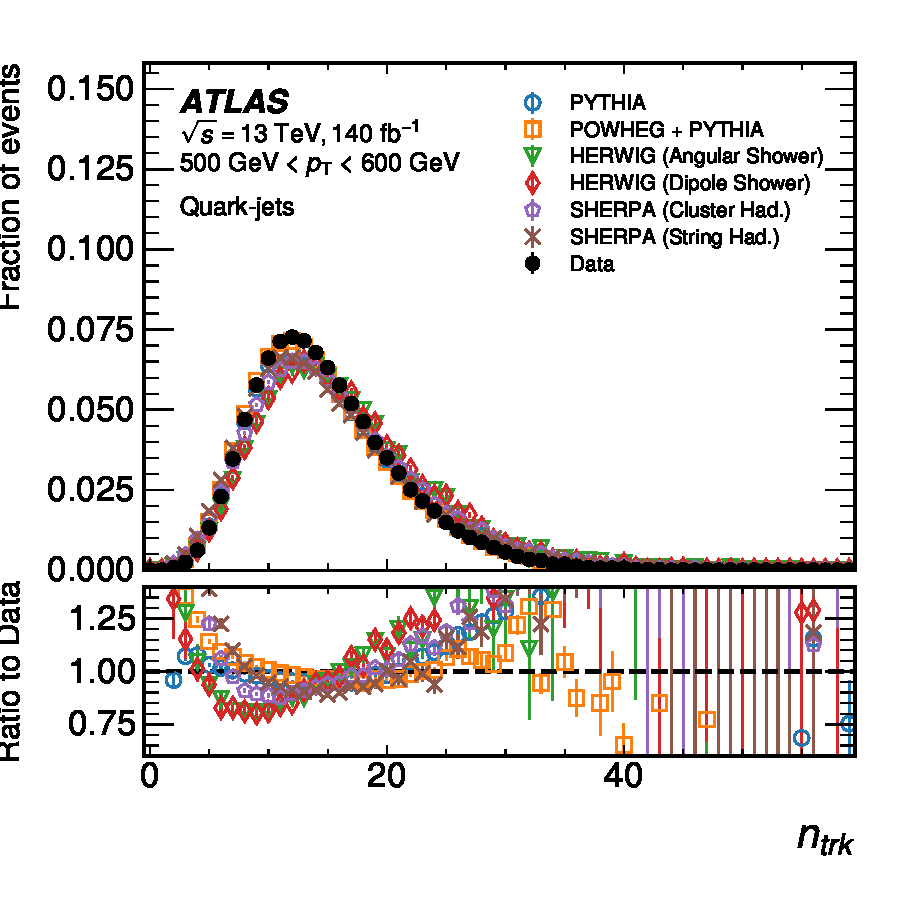
\includegraphics[width=0.45\textwidth]{fig/mcclosure_gen/mcclosure_jet_nTracks_jet_nTracks_Quark_500_data.pdf}} \quad
	\subfloat[]{\label{fig:roc-bdt12}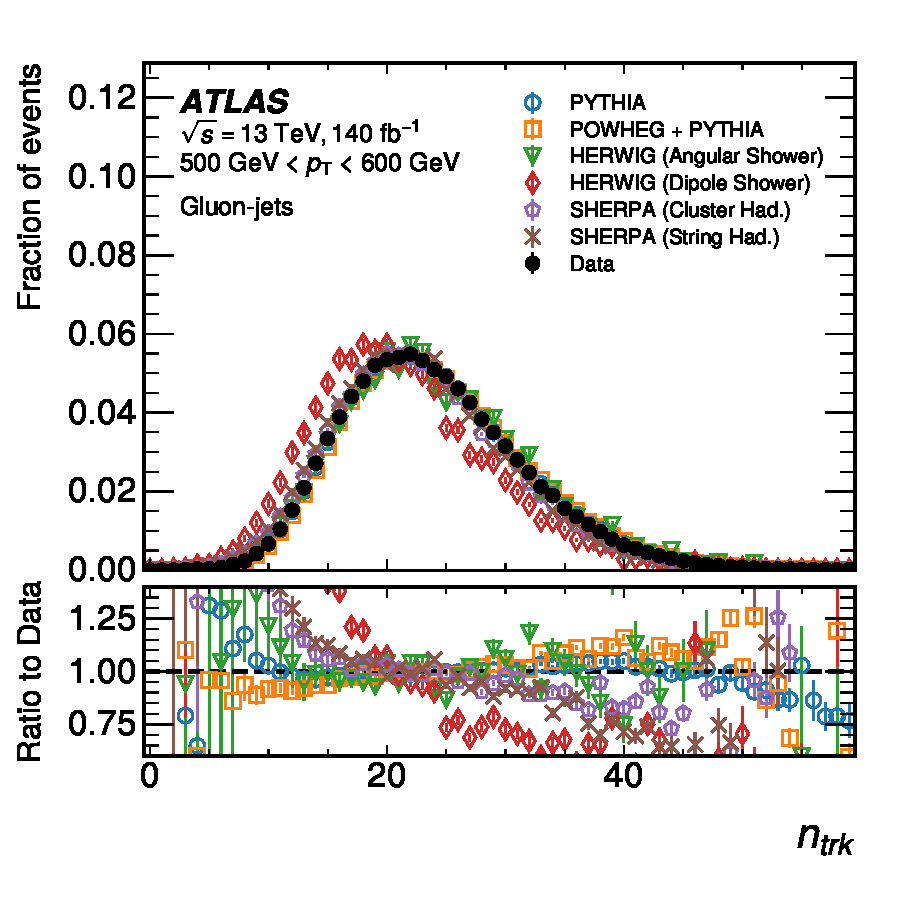
\includegraphics[width=0.45\textwidth]{fig/mcclosure_gen/mcclosure_jet_nTracks_jet_nTracks_Gluon_500_data.pdf}}\\
	\subfloat[]{\label{fig:roc-ntrk22}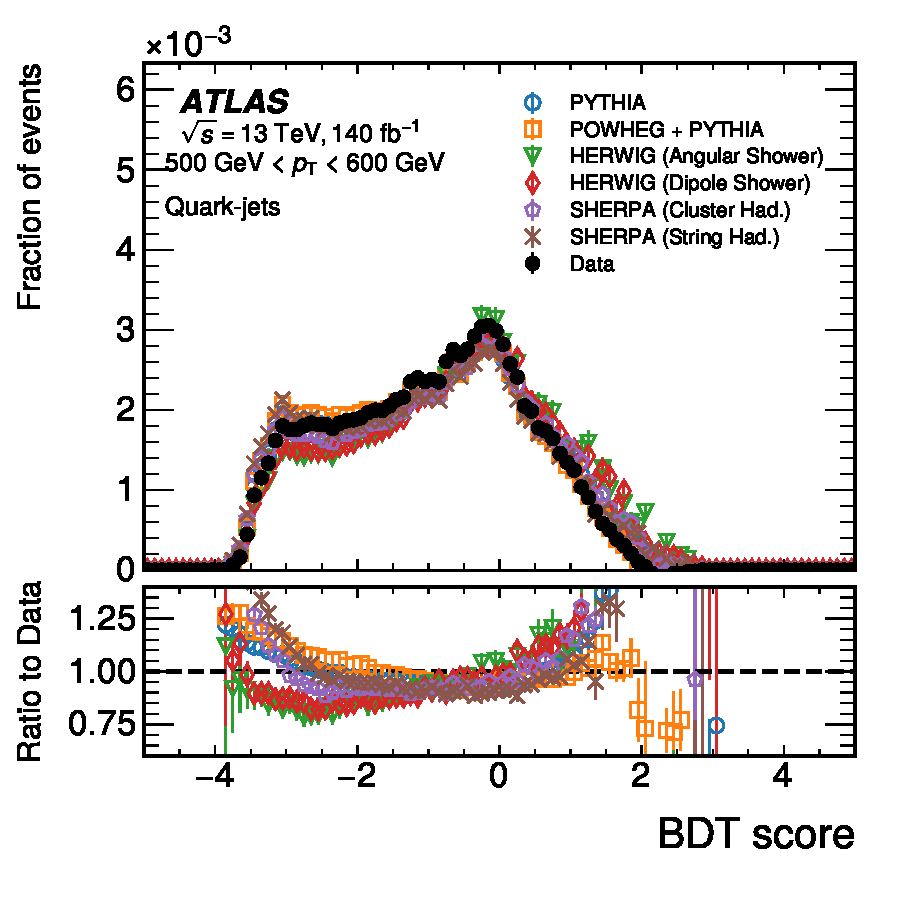
\includegraphics[width=0.45\textwidth]{fig/mcclosure_gen/mcclosure_GBDT_newScore_GBDT_newScore_Quark_500_data.pdf}} \quad
	\subfloat[]{\label{fig:roc-bdt22}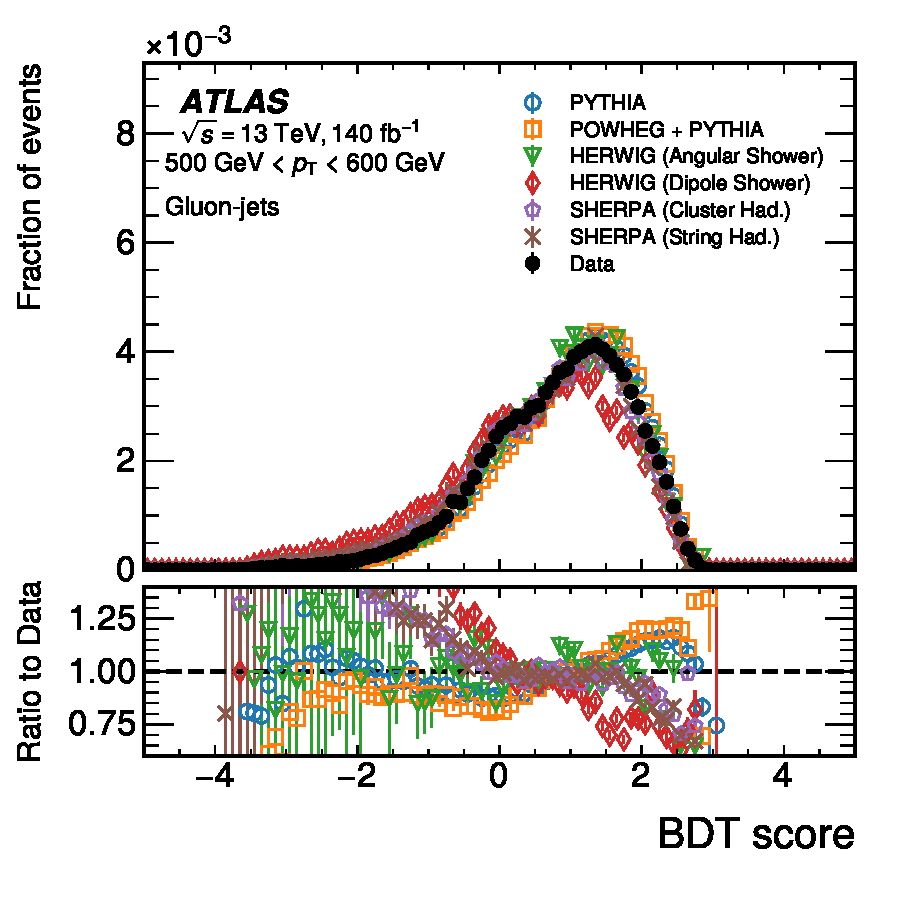
\includegraphics[width=0.45\textwidth]{fig/mcclosure_gen/mcclosure_GBDT_newScore_GBDT_newScore_Gluon_500_data.pdf}}
	\caption[]{
		The distributions of \ntrk~(a,b) and BDT score (c,d) for quark-jets (left) and gluon-jets (right) using different generators (open symbols) and data (closed symbol) are shown in the upper panels. The lower panels show the ratio of each MC distribution and the data. The vertical error bars show the statistical uncertainty.%
		%.
		\label{fig:QG-roc-com12}
	}
\end{figure}


\begin{figure}[htb]
	\centering
	\subfloat[]{\label{fig:roc-ntrk12}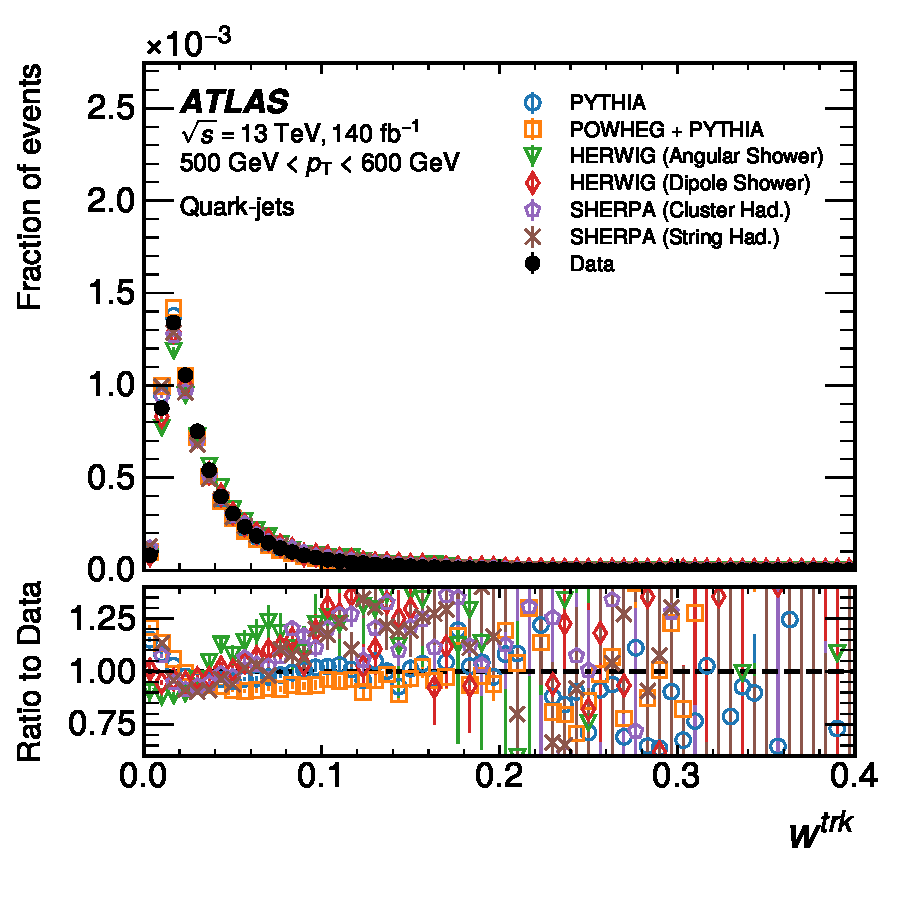
\includegraphics[width=0.45\textwidth]{fig/mcclosure_gen/mcclosure_jet_nTracks_jet_trackWidth_Quark_500_data.pdf}}\quad
	\subfloat[]{\label{fig:roc-bdt12}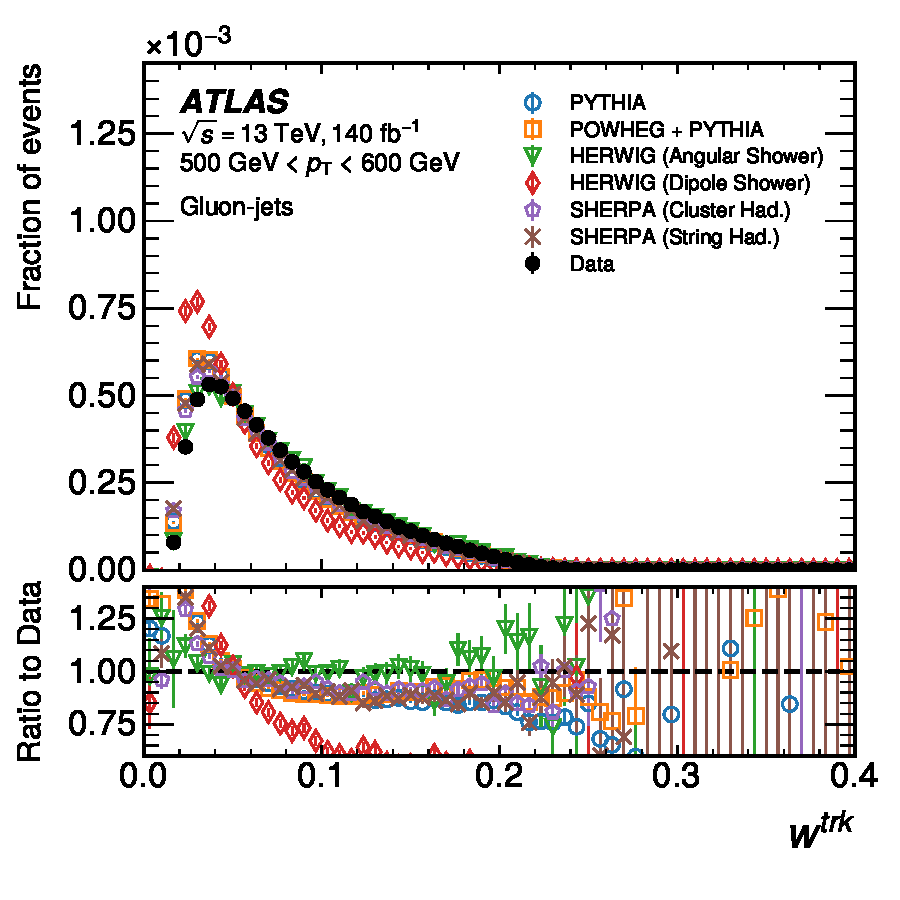
\includegraphics[width=0.45\textwidth]{fig/mcclosure_gen/mcclosure_jet_nTracks_jet_trackWidth_Gluon_500_data.pdf}}\\
	\subfloat[]{\label{fig:roc-ntrk22}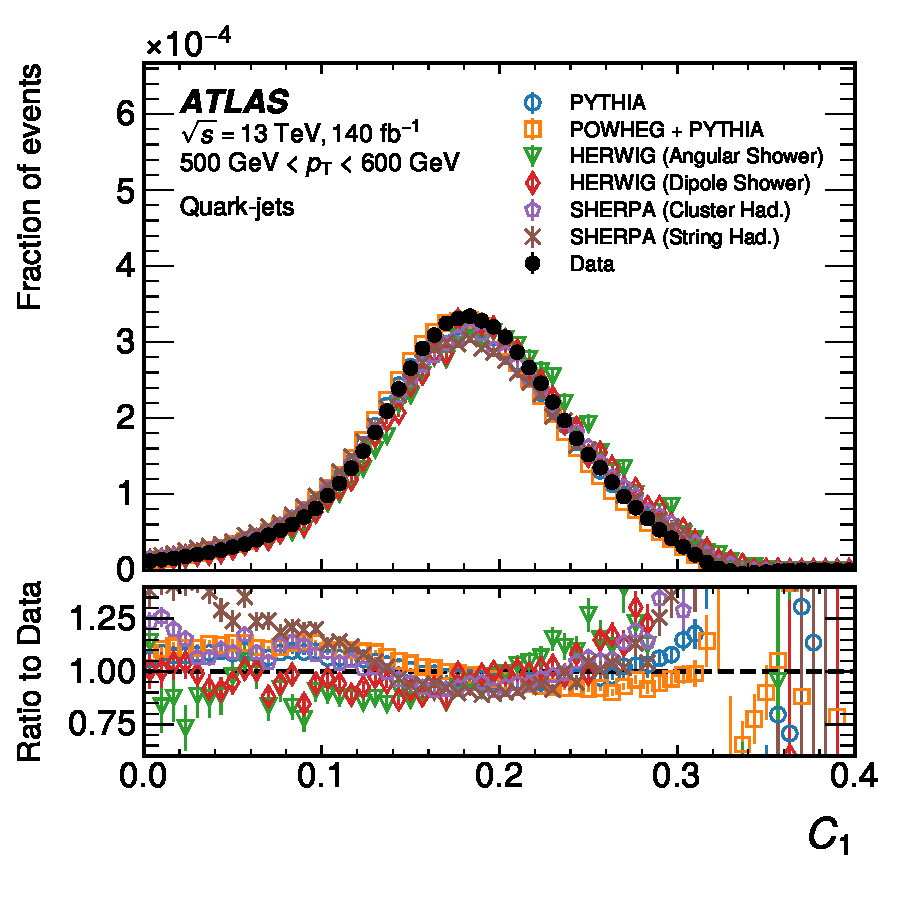
\includegraphics[width=0.45\textwidth]{fig/mcclosure_gen/mcclosure_GBDT_newScore_jet_trackC1_Quark_500_data.pdf}}\quad
	\subfloat[]{\label{fig:roc-bdt22}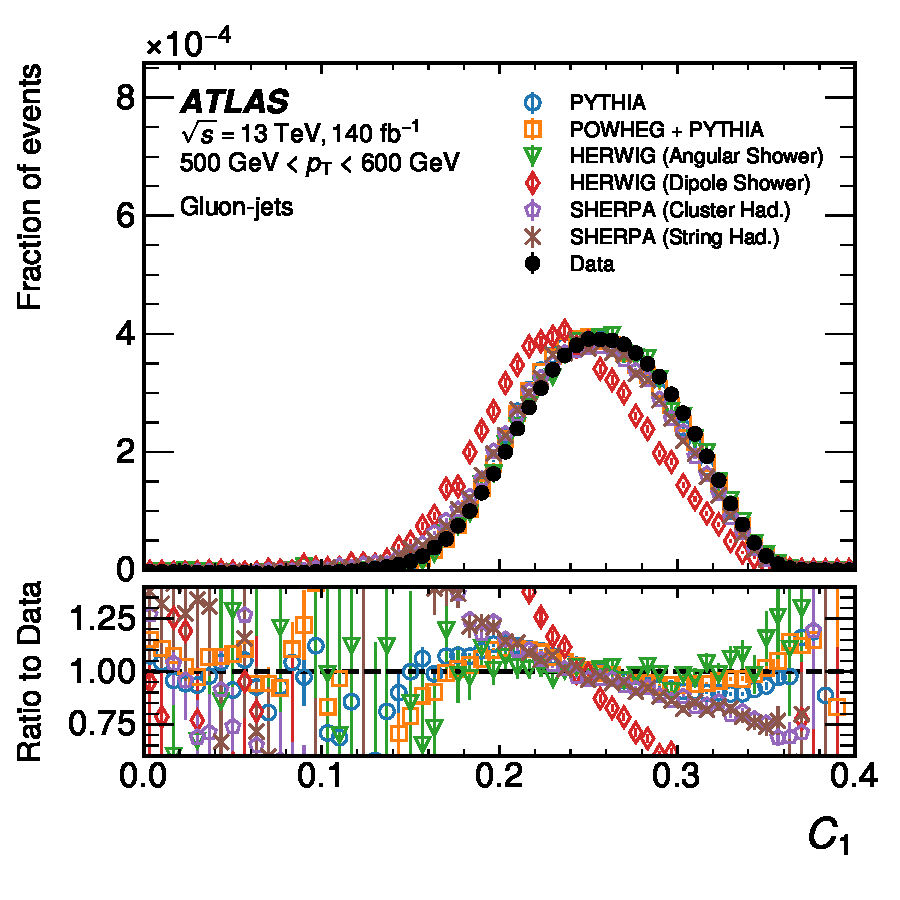
\includegraphics[width=0.45\textwidth]{fig/mcclosure_gen/mcclosure_GBDT_newScore_jet_trackC1_Gluon_500_data.pdf}}
	\caption[]{
		The distributions of \wtrk~(a,b) and $C_1$ (c,d) for quark-jets (left) and gluon-jets (right) using different generators (open symbols) and data (closed symbol) are shown in the upper panels. The lower panels show the ratio of each MC distribution and the data. The vertical error bars show the statistical uncertainty.%
		%.
		\label{fig:QG-roc-com122}
	}
\end{figure}

\begin{figure}[htb]
	\centering
	\subfloat[]{\label{fig:roc-ntrk12}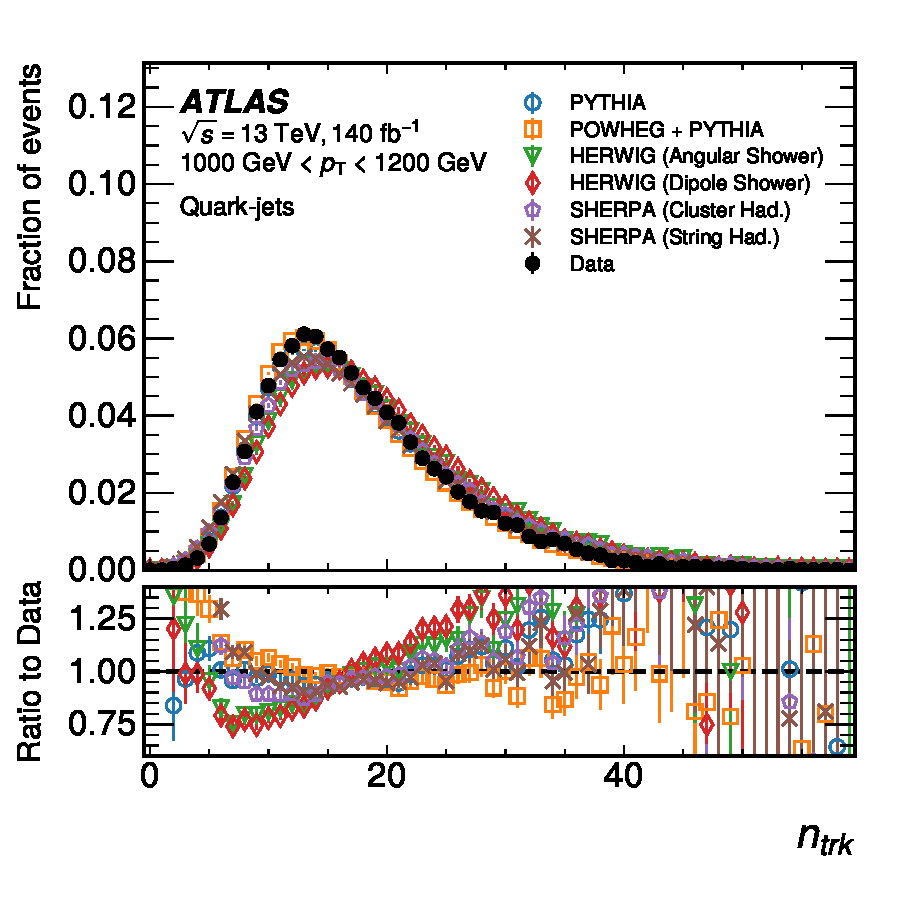
\includegraphics[width=0.45\textwidth]{fig/mcclosure_gen/mcclosure_jet_nTracks_jet_nTracks_Quark_1000_data.pdf}} \quad
	\subfloat[]{\label{fig:roc-bdt12}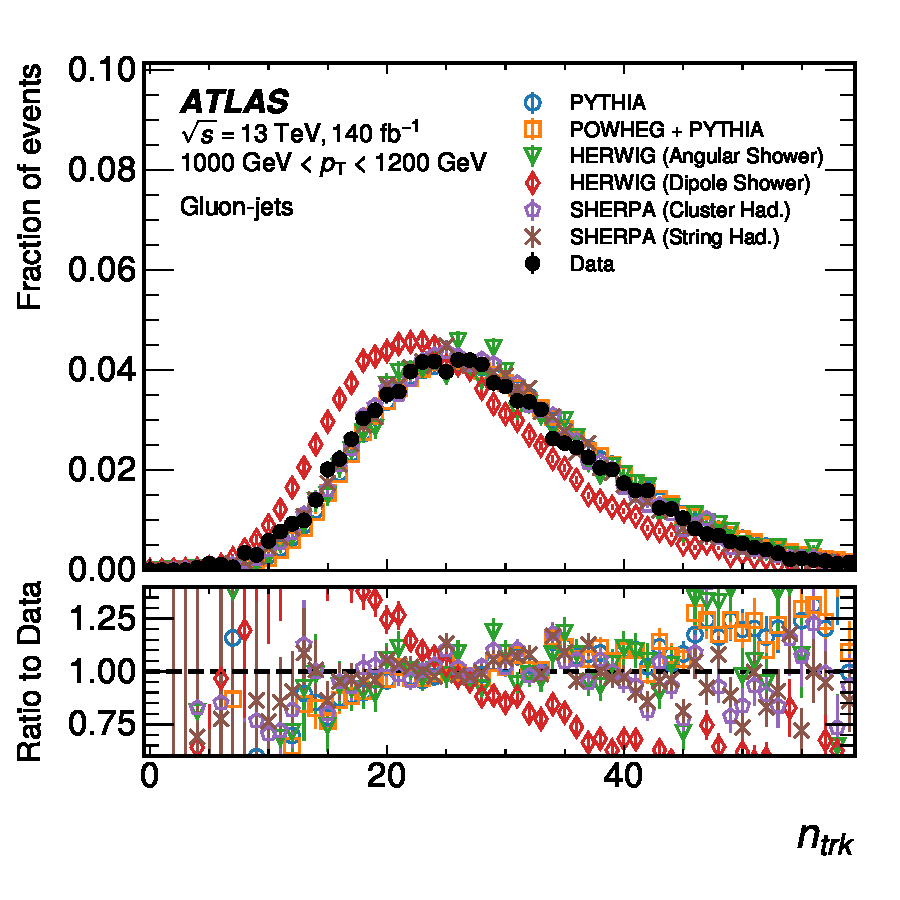
\includegraphics[width=0.45\textwidth]{fig/mcclosure_gen/mcclosure_jet_nTracks_jet_nTracks_Gluon_1000_data.pdf}}\\
	\subfloat[]{\label{fig:roc-ntrk22}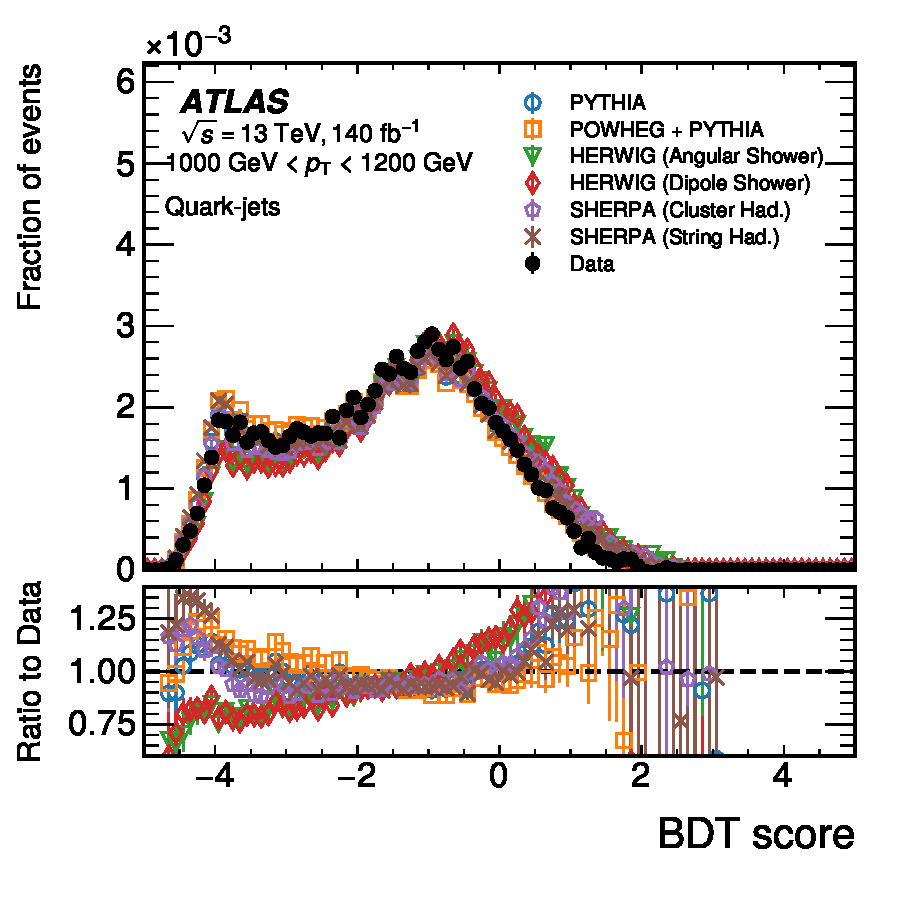
\includegraphics[width=0.45\textwidth]{fig/mcclosure_gen/mcclosure_GBDT_newScore_GBDT_newScore_Quark_1000_data.pdf}} \quad
	\subfloat[]{\label{fig:roc-bdt22}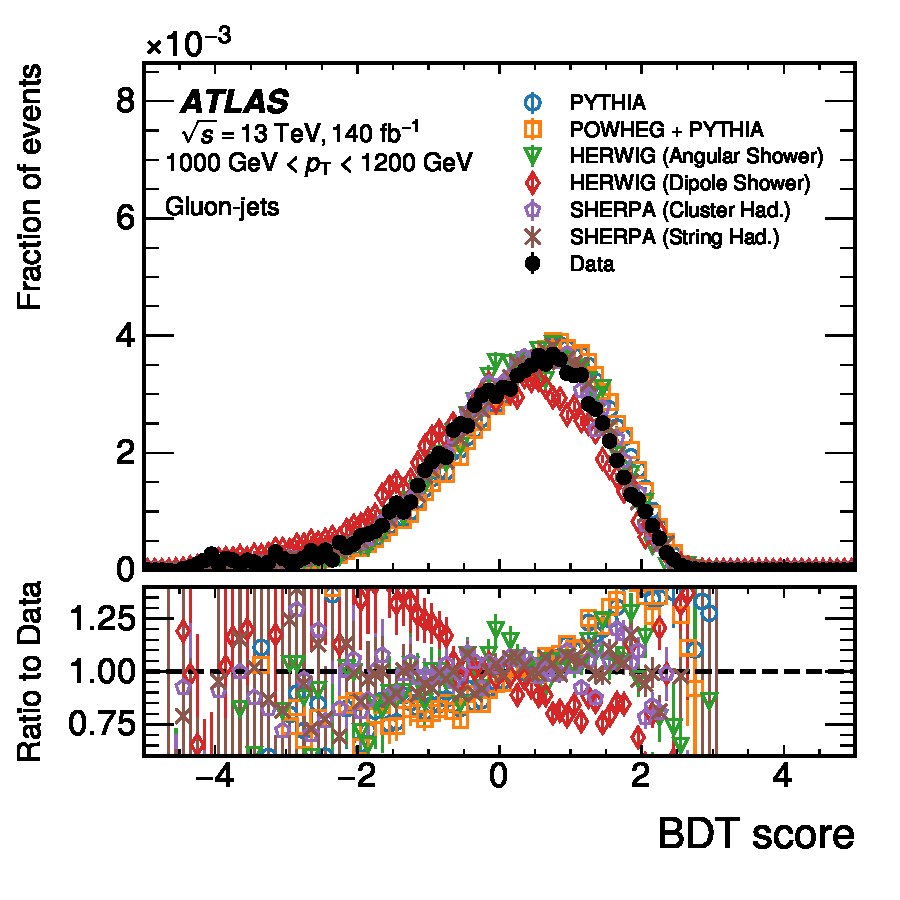
\includegraphics[width=0.45\textwidth]{fig/mcclosure_gen/mcclosure_GBDT_newScore_GBDT_newScore_Gluon_1000_data.pdf}}
	\caption[]{
		The distributions of \ntrk~(a,b) and BDT score (c,d) for quark-jets (left) and gluon-jets (right) using different generators (open symbols) and data (closed symbol) are shown in the upper panels. The lower panels show the ratio of each MC distribution and the data. The vertical error bars show the statistical uncertainty.%
		%.
		\label{fig:QG-roc-com121}
	}
\end{figure}


\begin{figure}[htb]
	\centering
	\subfloat[]{\label{fig:roc-ntrk12}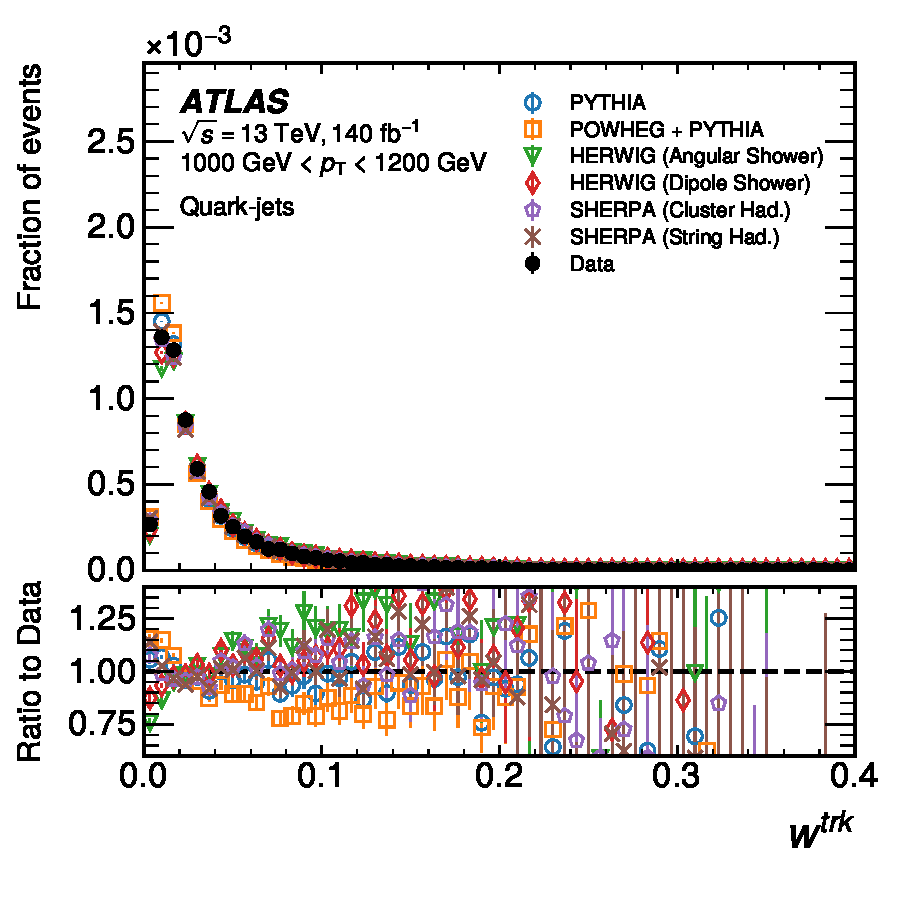
\includegraphics[width=0.45\textwidth]{fig/mcclosure_gen/mcclosure_jet_nTracks_jet_trackWidth_Quark_1000_data.pdf}}\quad
	\subfloat[]{\label{fig:roc-bdt12}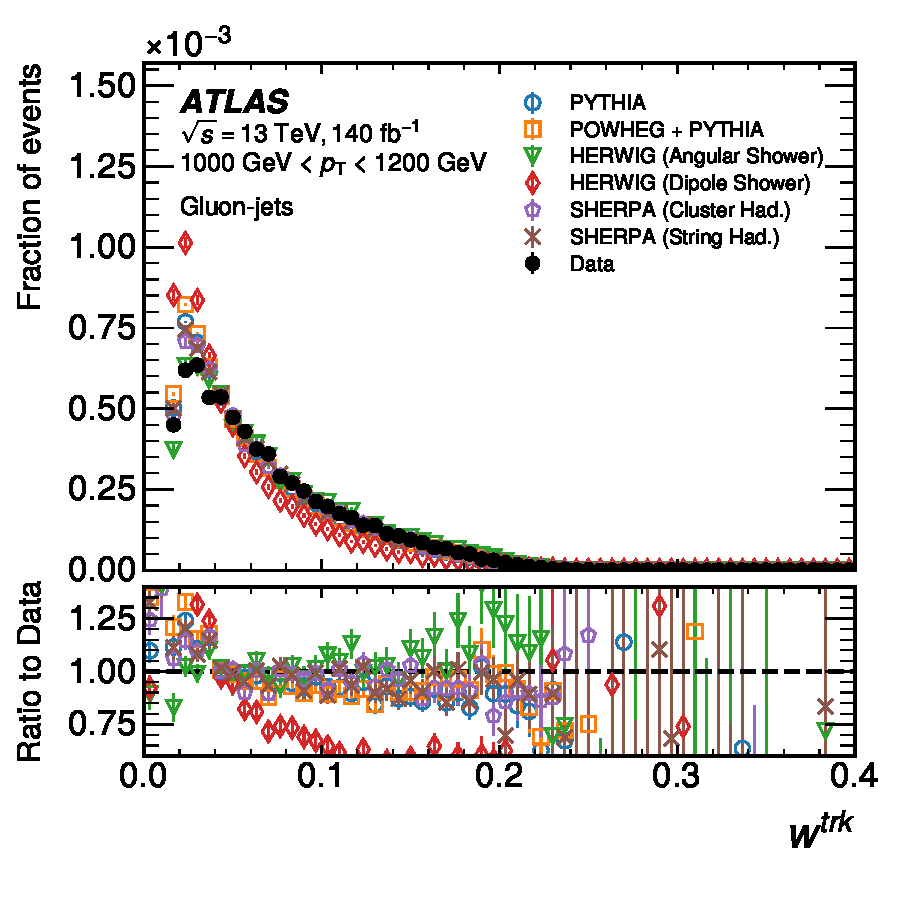
\includegraphics[width=0.45\textwidth]{fig/mcclosure_gen/mcclosure_jet_nTracks_jet_trackWidth_Gluon_1000_data.pdf}}\\
	\subfloat[]{\label{fig:roc-ntrk22}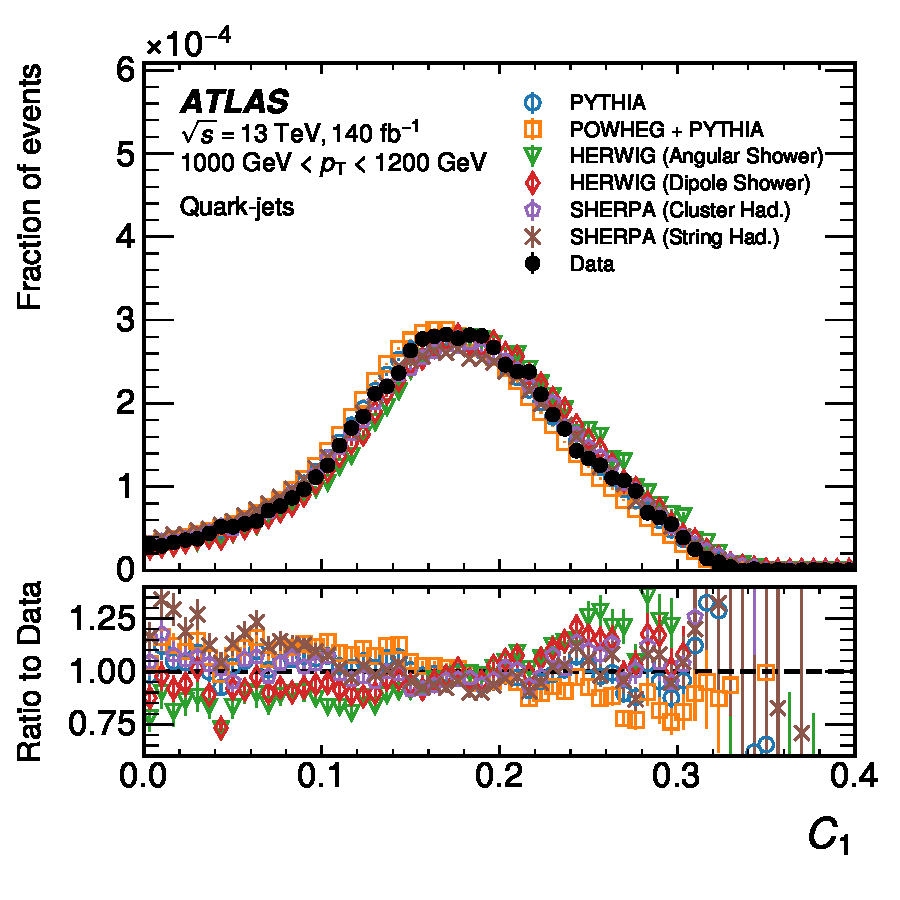
\includegraphics[width=0.45\textwidth]{fig/mcclosure_gen/mcclosure_GBDT_newScore_jet_trackC1_Quark_1000_data.pdf}}\quad
	\subfloat[]{\label{fig:roc-bdt22}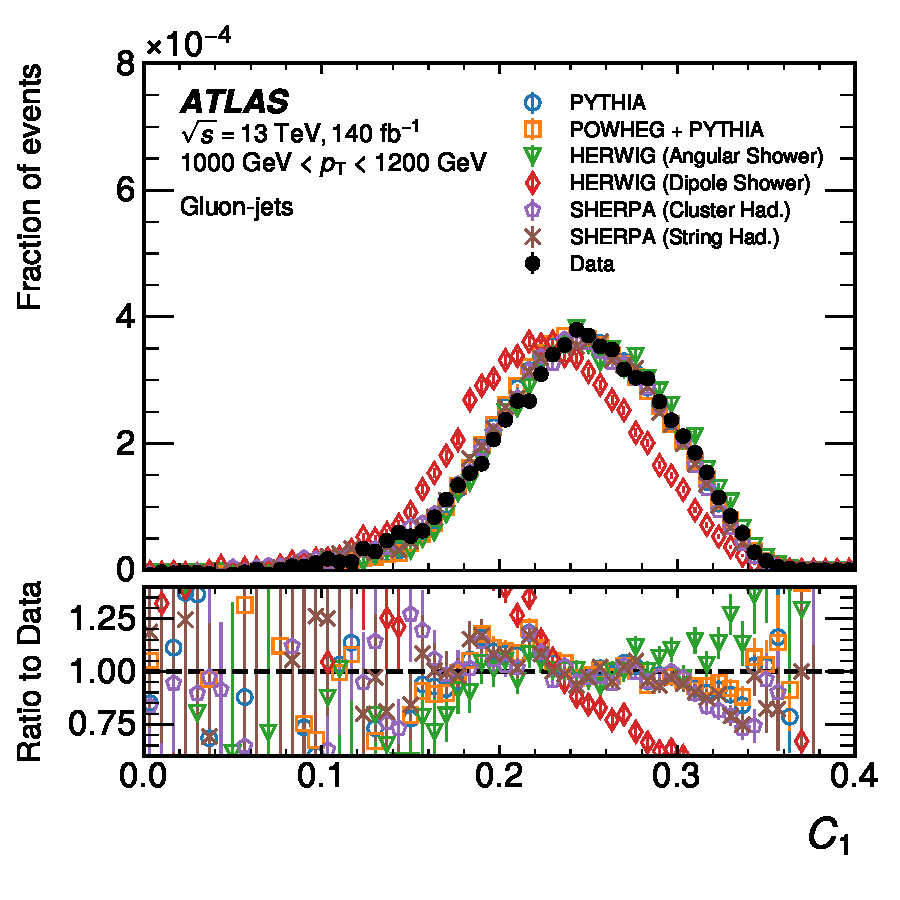
\includegraphics[width=0.45\textwidth]{fig/mcclosure_gen/mcclosure_GBDT_newScore_jet_trackC1_Gluon_1000_data.pdf}}
	\caption[]{
		The distributions of \wtrk~(a,b) and $C_1$ (c,d) for quark-jets (left) and gluon-jets (right) using different generators (open symbols) and data (closed symbol) are shown in the upper panels. The lower panels show the ratio of each MC distribution and the data. The vertical error bars show the statistical uncertainty.%
		%.
		\label{fig:QG-roc-com1211}
	}
\end{figure}


\FloatBarrier
Cut values corresponding to the 50\% WP are summarised in Table~\ref{tab:wp-ntrk} for the \ntrk-only tagger and Table~\ref{tab:wp-bdt} for the BDT-tagger. Figure~\ref{fig:QG-pythia-Unc_Ntrk-wp} shows the gluon-jets efficiency of both \ntrk-only tagger and the BDT-tagger as a function of jet \pt, for the MC and data, at four WPs.


Both the \ntrk-only and BDT-taggers demonstrate commendable performance on data, with high quark signal efficiency across all \pt~range. Notably, at the 50\% working point, the \ntrk-only tagger achieves approximately 90\% rejection of gluon-jets, while the BDT tagger surpasses this performance by rejecting around 93\% of gluon-jets. The BDT-tagger outperforms the {\ntrk}-only tagger by exhibiting superior gluon-jets rejection rates at the identical WP. This disparity in performance arises from the inclusion of a more comprehensive set of jet substructure variables in the BDT approach. The discrepancy between the level of gluon-jet rejection observed in data and that predicted by the MC samples increases as the jet \pt~increases. This phenomenon is closely tied to the dissimilarity between the modelling of gluons and their actual behaviour in data.



\begin{table}[htb]
	\centering
    \resizebox{0.95\textwidth}{!}{
	\begin{tabular}{c|ccccccc}
		\hline
		\hline
		\pt~[GeV]& 500 - 600 & 600 - 800 & 800 - 1000 & 1000 - 1200 & 1200 - 1500 & 1500 - 2000\\\hline
		\hline
		WP& &&&&& \\
		0.5&15.0 & 16.0 & 17.0 & 18.0 & 18.0 & 19.0\\
		0.6&17.0 & 18.0 & 19.0 & 20.0 & 20.0 & 21.0\\
		0.7&19.0 & 20.0 & 21.0 & 22.0 & 23.0 & 24.0\\
		0.8&22.0 & 23.0 & 24.0 & 26.0 & 27.0 & 28.0\\\hline\hline
	\end{tabular}}
	\caption{Cut values of \ntrk~at different working point in each of jet \pt~range}
	\label{tab:wp-ntrk}
\end{table}


\begin{table}[htb]
	\centering
    \resizebox{0.95\textwidth}{!}{
	\begin{tabular}{c|ccccccc}
		\hline
		\hline
		\pt~[GeV]& 500 - 600 & 600 - 800 & 800 - 1000 & 1000 - 1200 & 1200 - 1500 & 1500 - 2000\\\hline
		\hline
		WP& &&&&& \\
		0.5&-0.8 & -1.0 & -1.2 & -1.4 & -1.6 & -1.8\\
		0.6&-0.4 & -0.6 & -0.8 & -1.0 & -1.2 & -1.4\\
		0.7&0.0 & -0.2 & -0.4 & -0.6 & -0.8 & -1.0\\
		0.8&0.4 & 0.2 & 0.0 & -0.2 & -0.3 & -0.6
		\\\hline\hline
	\end{tabular}}
	\caption{Cut values of BDT at different working point in each of jet \pt~range}
	\label{tab:wp-bdt}
\end{table}




\begin{figure}[htbp]
	\centering
	\subfloat[Working Point:50\%]{\label{fig:QG5}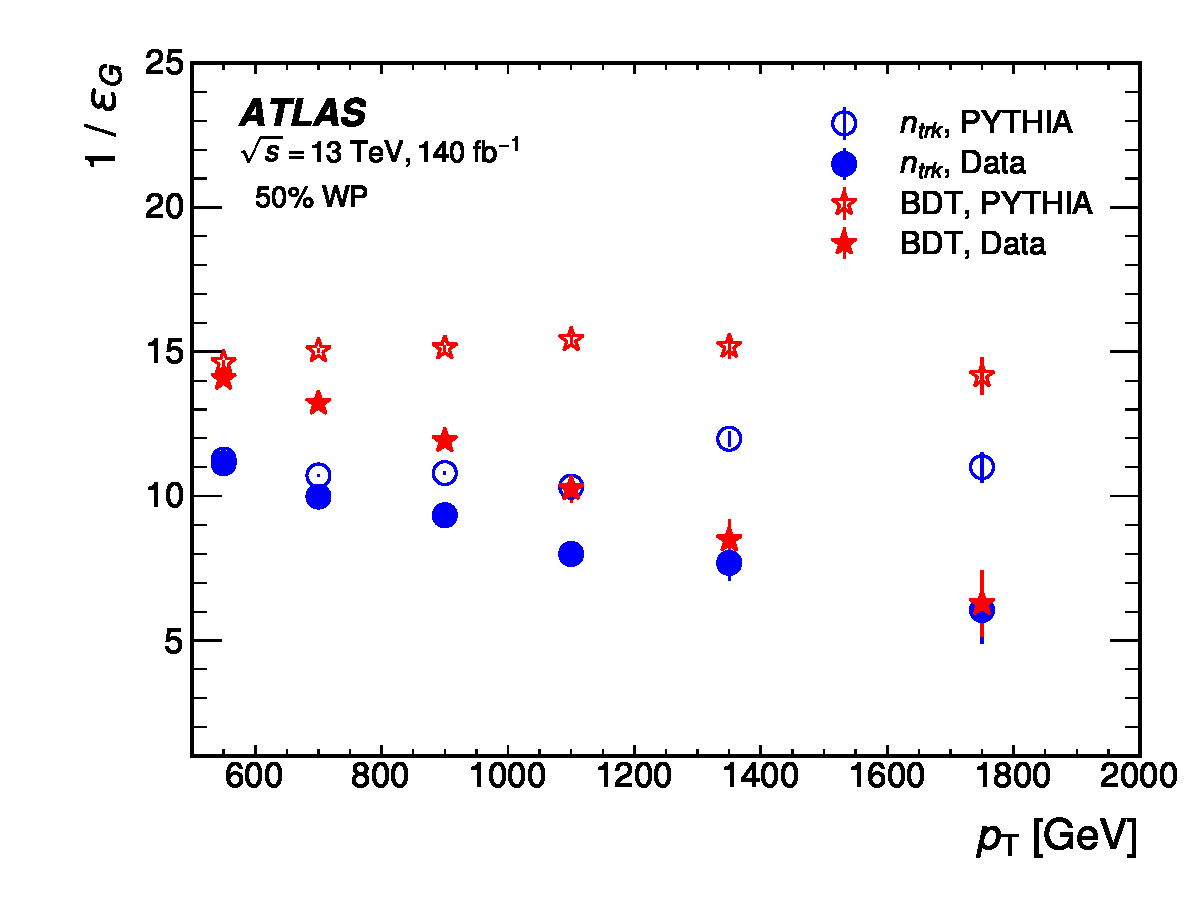
\includegraphics[width=0.45\textwidth]{fig/eff_gen/WP0.5.pdf}}\quad
	\subfloat[Working Point:60\%]{\label{fig:QG6}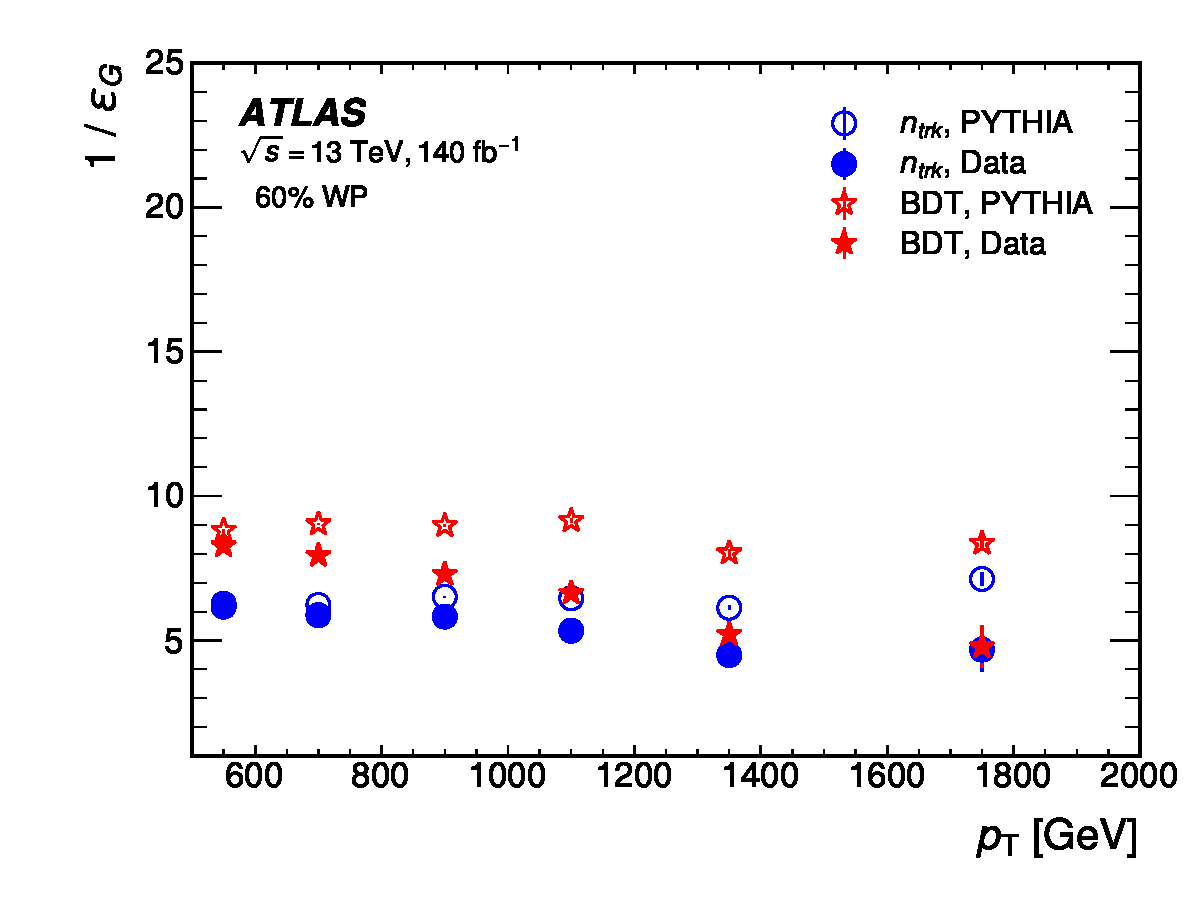
\includegraphics[width=0.45\textwidth]{fig/eff_gen/WP0.6.pdf}}\\
	\subfloat[Working Point:70\%]{\label{fig:QG5}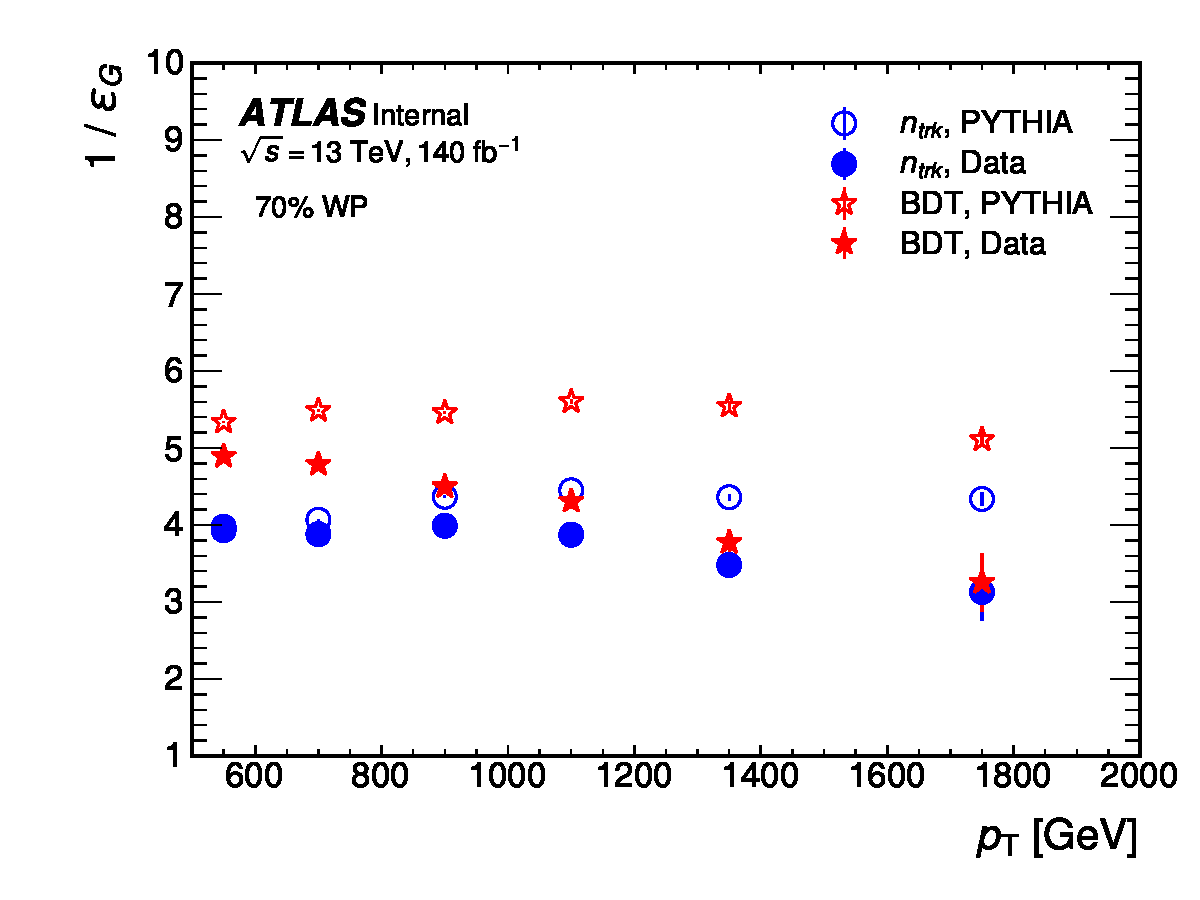
\includegraphics[width=0.45\textwidth]{fig/eff_gen/WP0.7.pdf}}\quad
	\subfloat[Working Point:80\%]{\label{fig:QG6}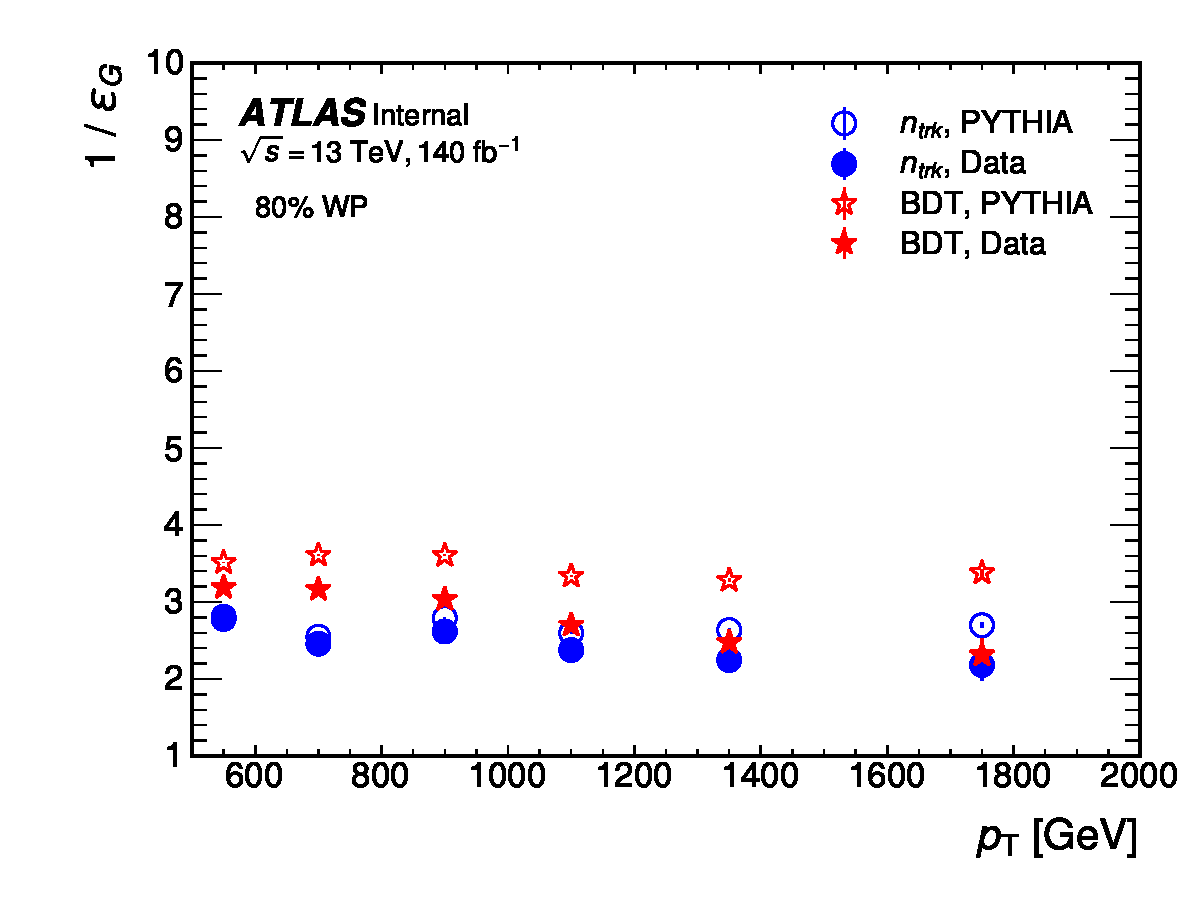
\includegraphics[width=0.45\textwidth]{fig/eff_gen/WP0.8.pdf}}
	\caption[]{
		Inverse of the gluon-jet efficiency of \ntrk~(circles) and BDT~(stars) as a function of jet \pt~at the each WP in data (closed symbols) and the \pythia~(open symbols) MC. The vertical error bars show the statistical uncertainty.
		\label{fig:QG-pythia-Unc_Ntrk-wp}
	}
\end{figure}







\FloatBarrier

%\subsubsection{Test the $\eta$ dependency of scale factors}
%\label{app:eta-dependency-section}
%
%
%The $\eta$ dependency of SFs is checked and described in Section~\ref{app:eta-dependency-section}. The difference in the SFs in different $\eta$ regions is not significant compared to the systematic uncertainties which are around 10\% and 20\% for quark and gluon jets respectively.
%
%The jet fragmentation is expected to be independent of $\eta$. To check the $\eta$ dependency on scale factors, the quark-enriched and gluon-enriched samples are further divided into two $\eta$ regions. The first region requires the central jet in 0 < $\mid\eta\mid$ < 0.5 and the forward jet in 0.5 < $\mid\eta\mid$ < 1 (0 < $\mid\eta_{C}\mid$ < 0.5,0.5 < $\mid\eta_{F}\mid$ < 1) and the second region requires the central jet in 0.5 < $\mid\eta\mid$ < 1 and the forward jet in 1 < $\mid\eta\mid$ < 2.1(0.5 < $\mid\eta_{C}\mid$ < 1,1 < $\mid\eta_{F}\mid$ < 2.1).  The distribution of $\ntrk$ and BDT score for jets in different $\eta$ ranges are shown in Fig.~\ref{fig:QG-pythia-etabin-ntrk-Pythia} and Fig.~\ref{fig:QG-pythia-etabin-BDT-Pythia}. The jets in second region has more track multiplicity than that in the first region as expected. 
%
%
%The working points are defined using the same procedure as the nominal result. The comparison of the SFs in different $\eta$ regions for different working points are shown in Fig.~\ref{fig:QG-pythia-eta-Ntrk-5} to \ref{fig:QG-pythia-eta-BDT-8}, the differences in SFs for different WPs are within 10\% and for quark and gluon jets in general. With considering the theoretical systematic uncertainty the differences are not significant. 
%More relevant studies are shown in Appendix ~\ref{app:eta-dependency-section-appendix}. 
%
%\begin{figure}[htb]
%	\centering
%	\subfloat[$Quark: 500<\pt<600\GeV$~(\pythia8)]{\label{fig:QG-pythia-NtrkDataQa}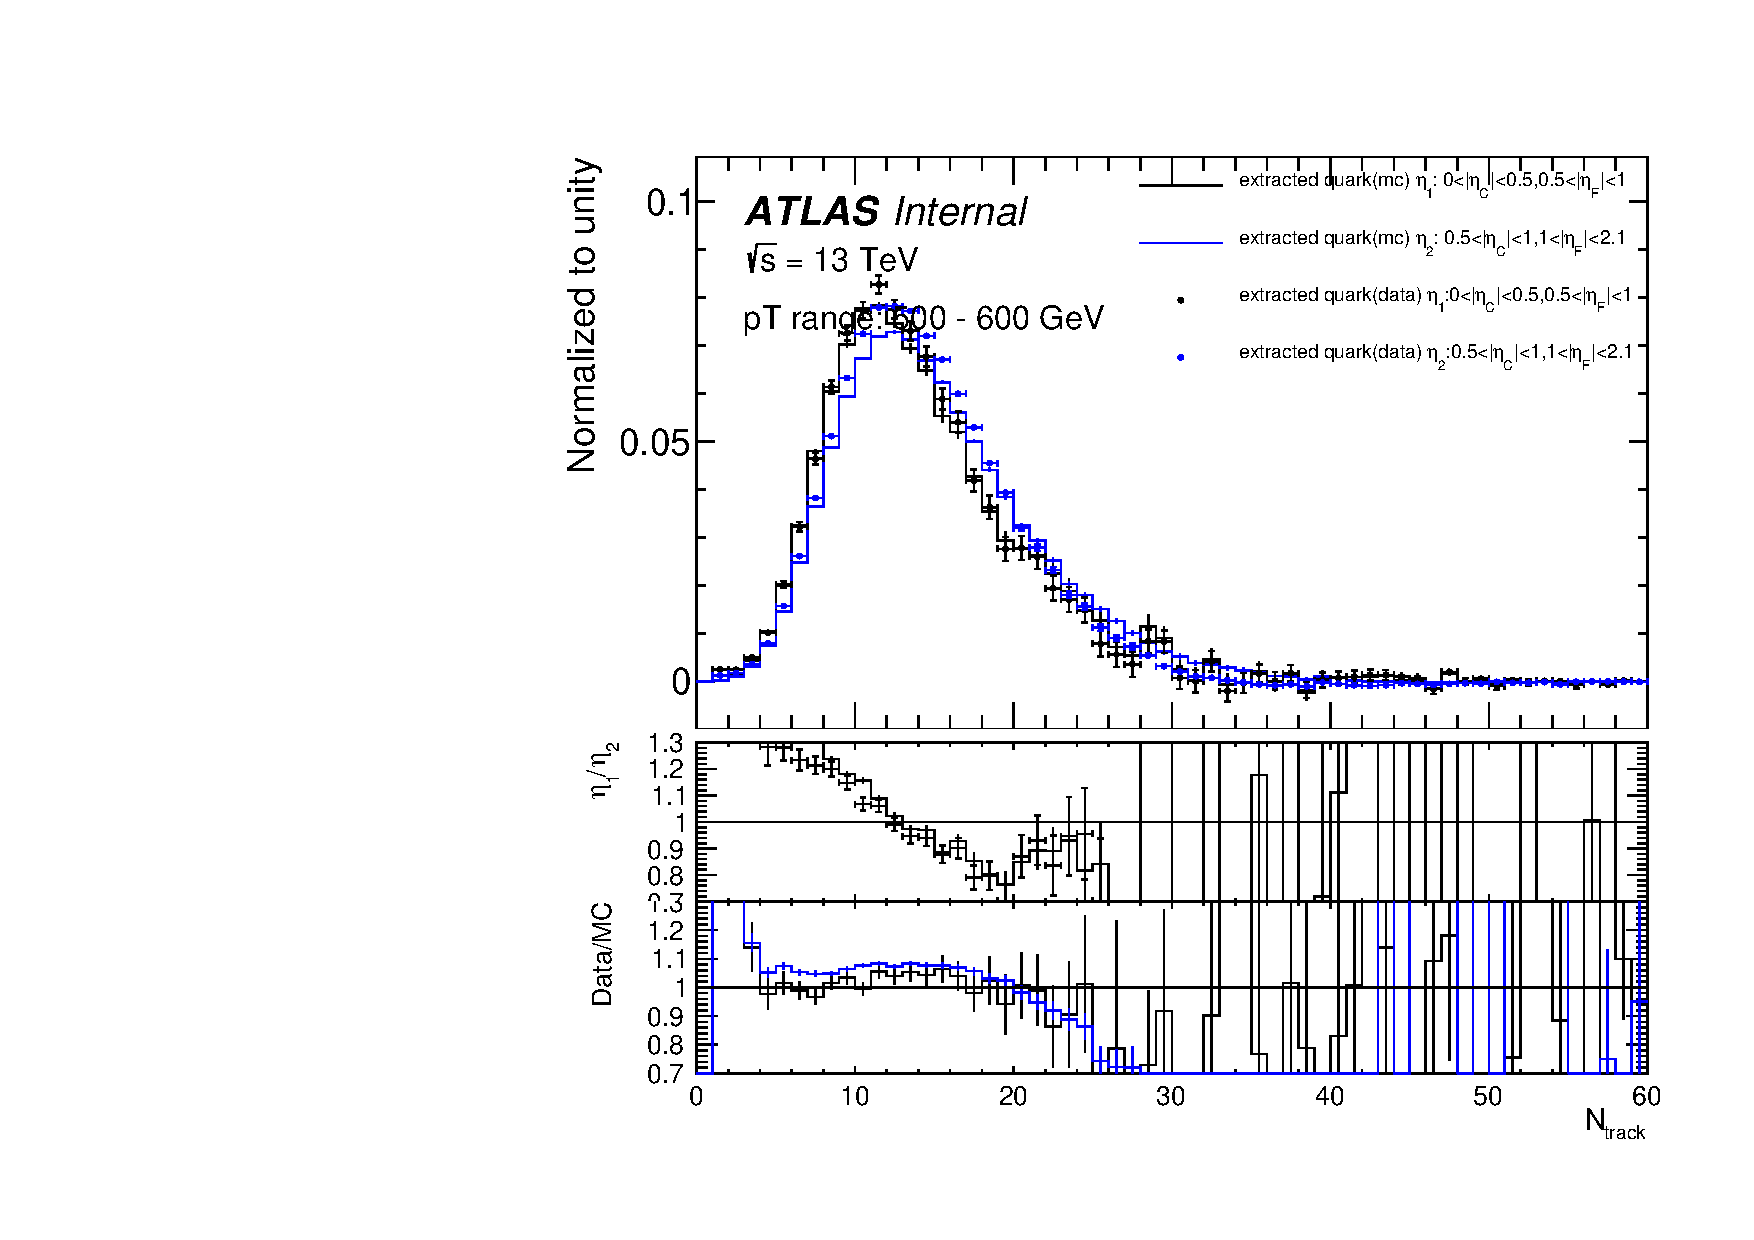
\includegraphics[width=0.45\textwidth]{fig/Method1/pythia/eta/extracted/plots_ntrk/quark_500_Quark_pythia_ntrk_compare_0-0.5_0.5-1_0.5-1_1-2.1.pdf}} \quad
%	\subfloat[$Gluon: 500<\pt<600\GeV$~(\pythia8)]{\label{fig:QG-pythia-NtrkDataGa}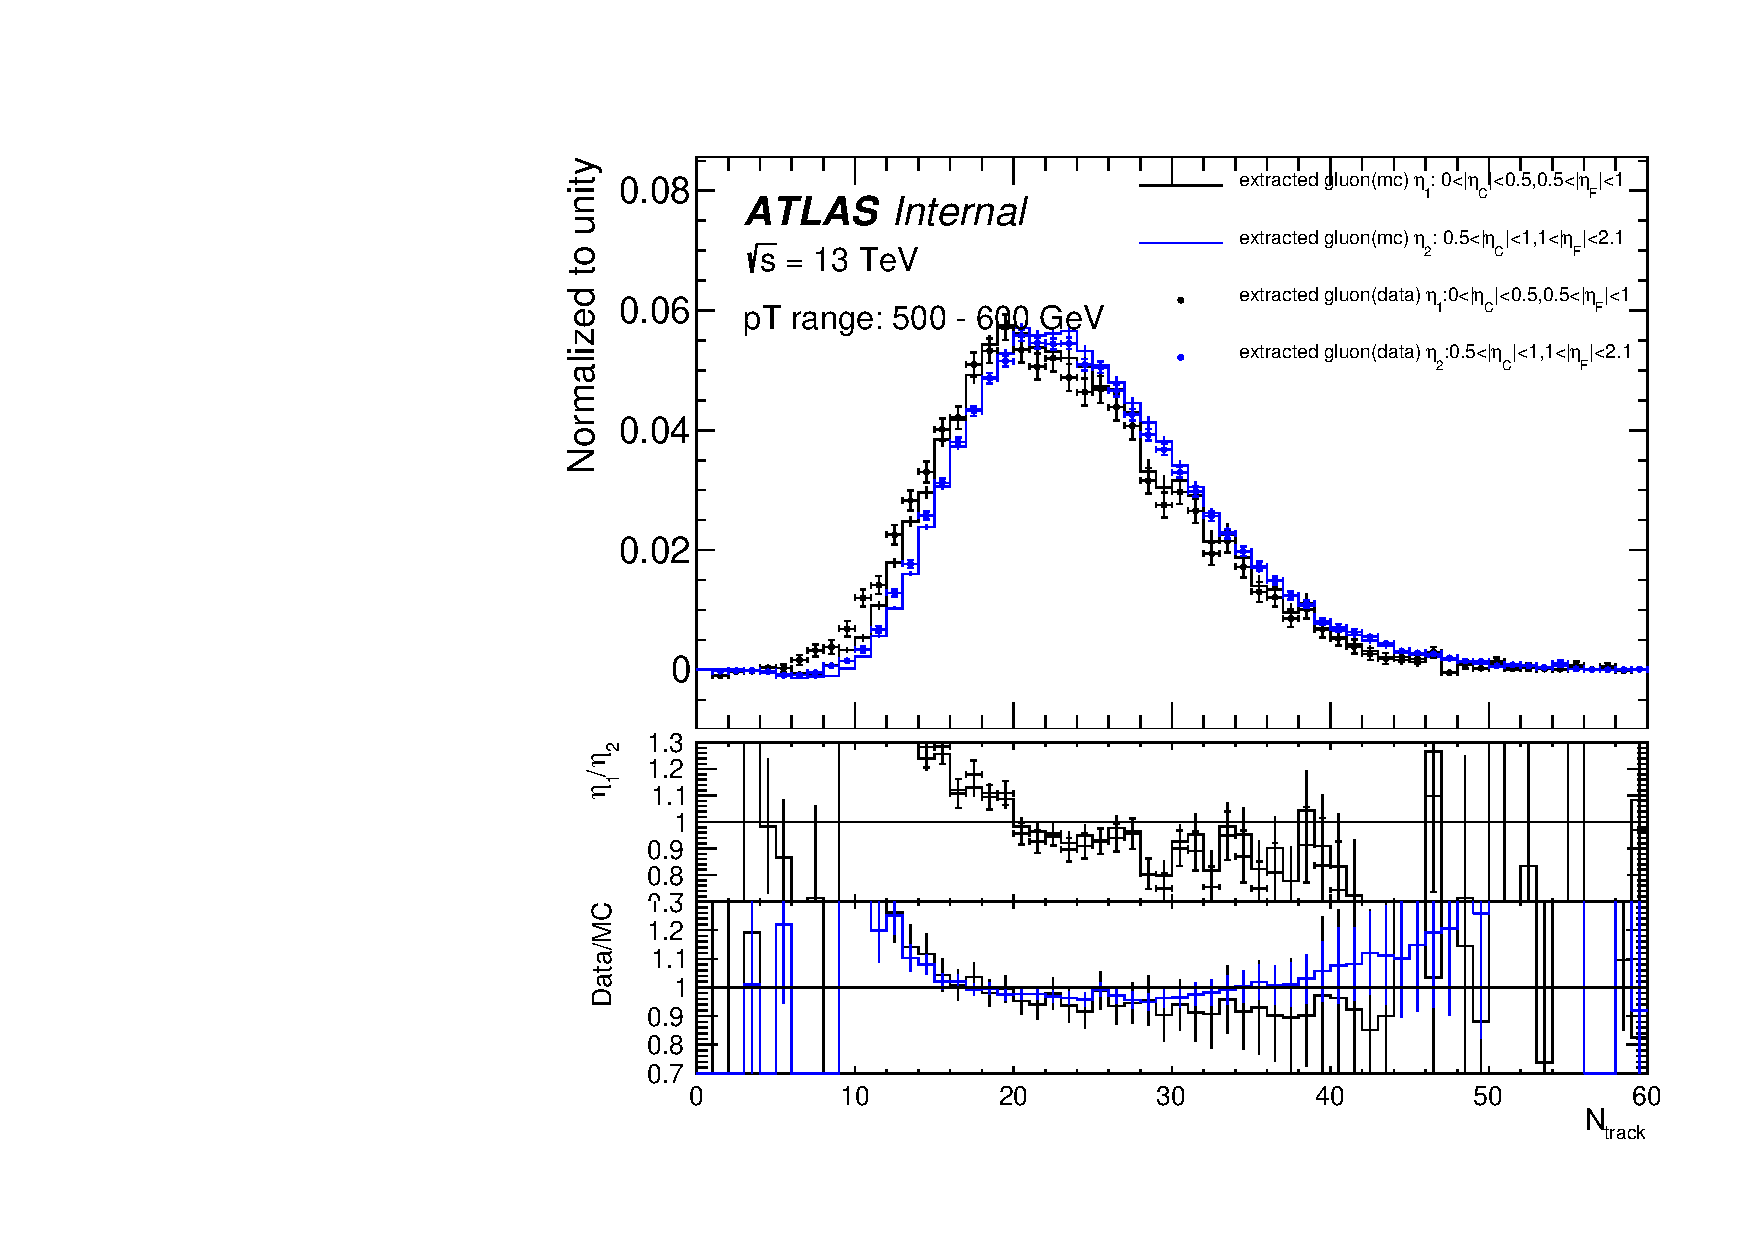
\includegraphics[width=0.45\textwidth]{fig/Method1/pythia/eta/extracted/plots_ntrk/gluon_500_Quark_pythia_ntrk_compare_0-0.5_0.5-1_0.5-1_1-2.1.pdf}}  \\
%	\subfloat[$Quark: 800<\pt<1000\GeV$~(\pythia8)]{\label{fig:QG-pythia-NtrkDataQb}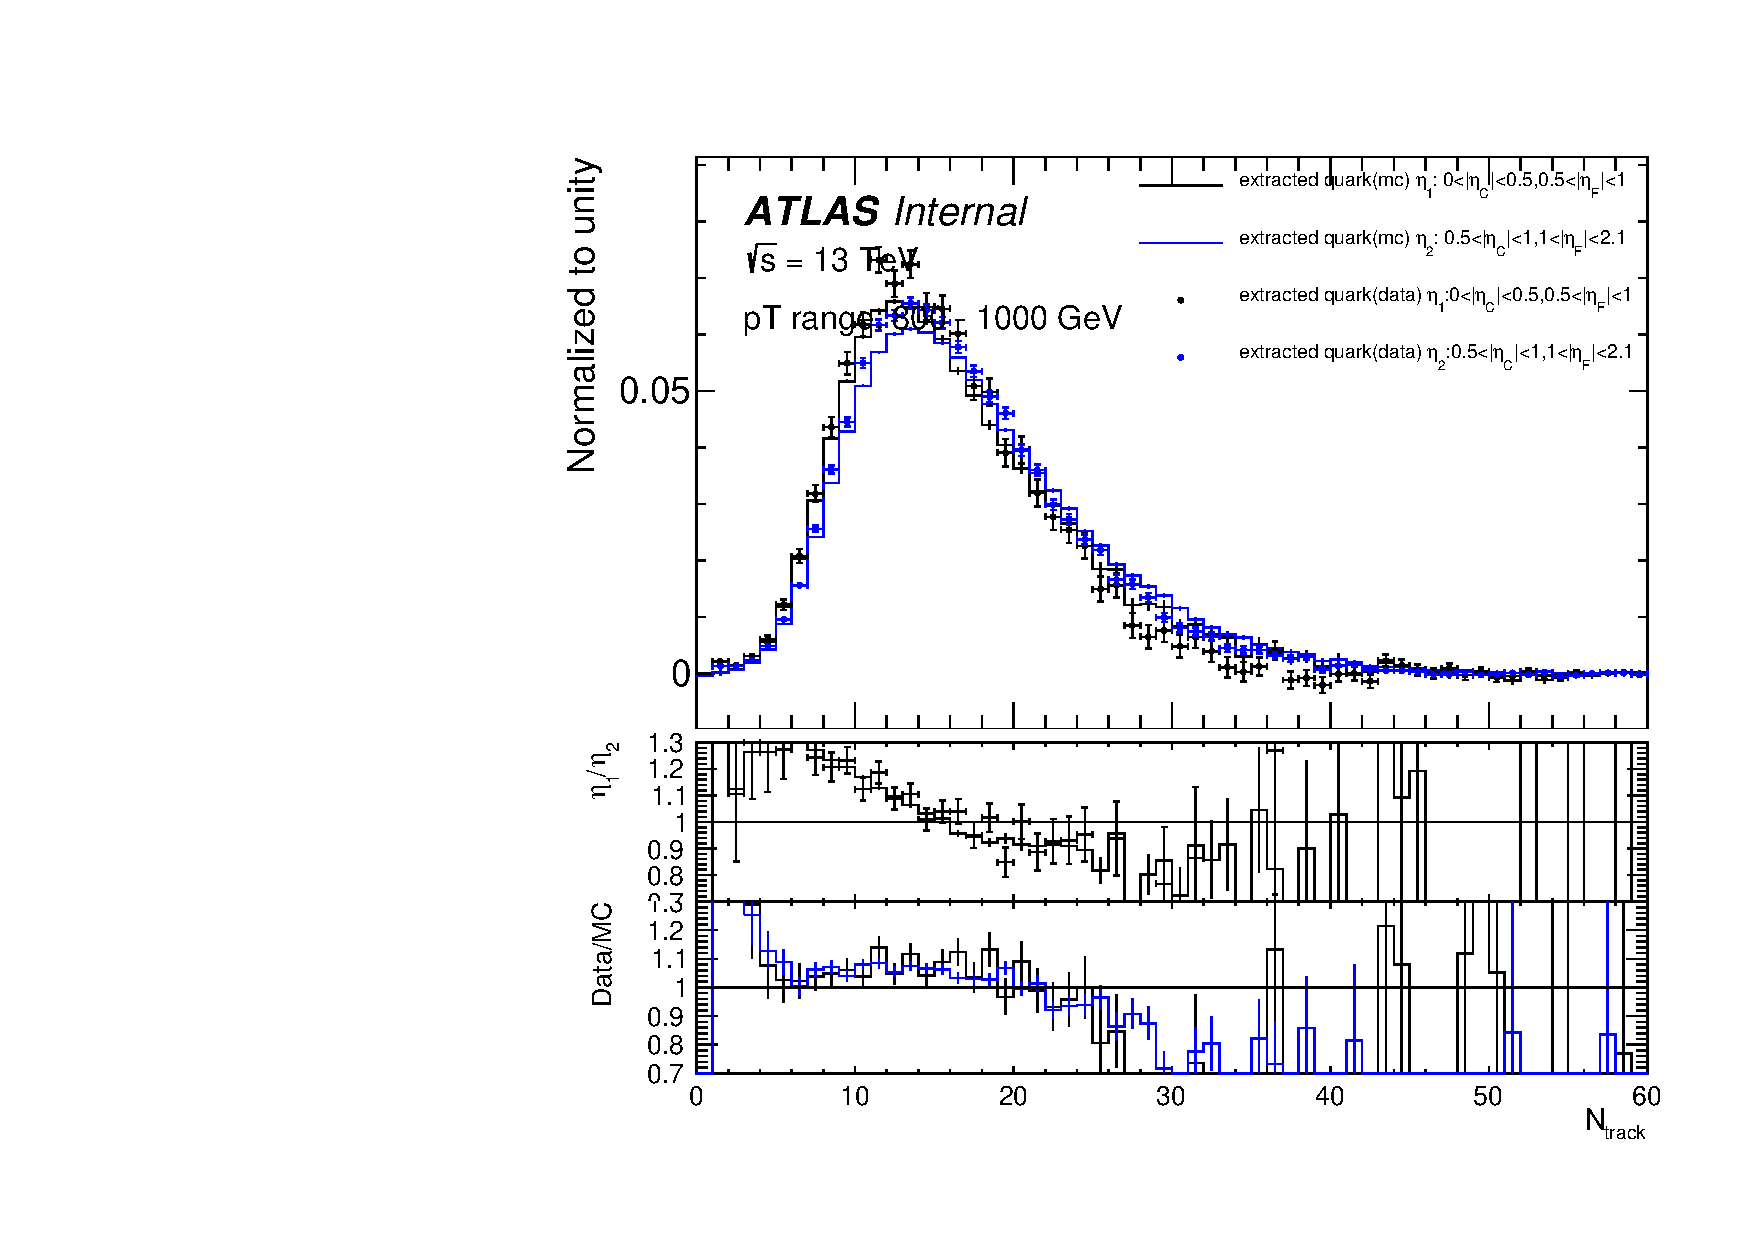
\includegraphics[width=0.45\textwidth]{fig/Method1/pythia/eta/extracted/plots_ntrk/quark_800_Quark_pythia_ntrk_compare_0-0.5_0.5-1_0.5-1_1-2.1.pdf}} \quad
%	\subfloat[$Gluon: 800<\pt<1000\GeV$~(\pythia8)]{\label{fig:QG-pythia-NtrkDataGb}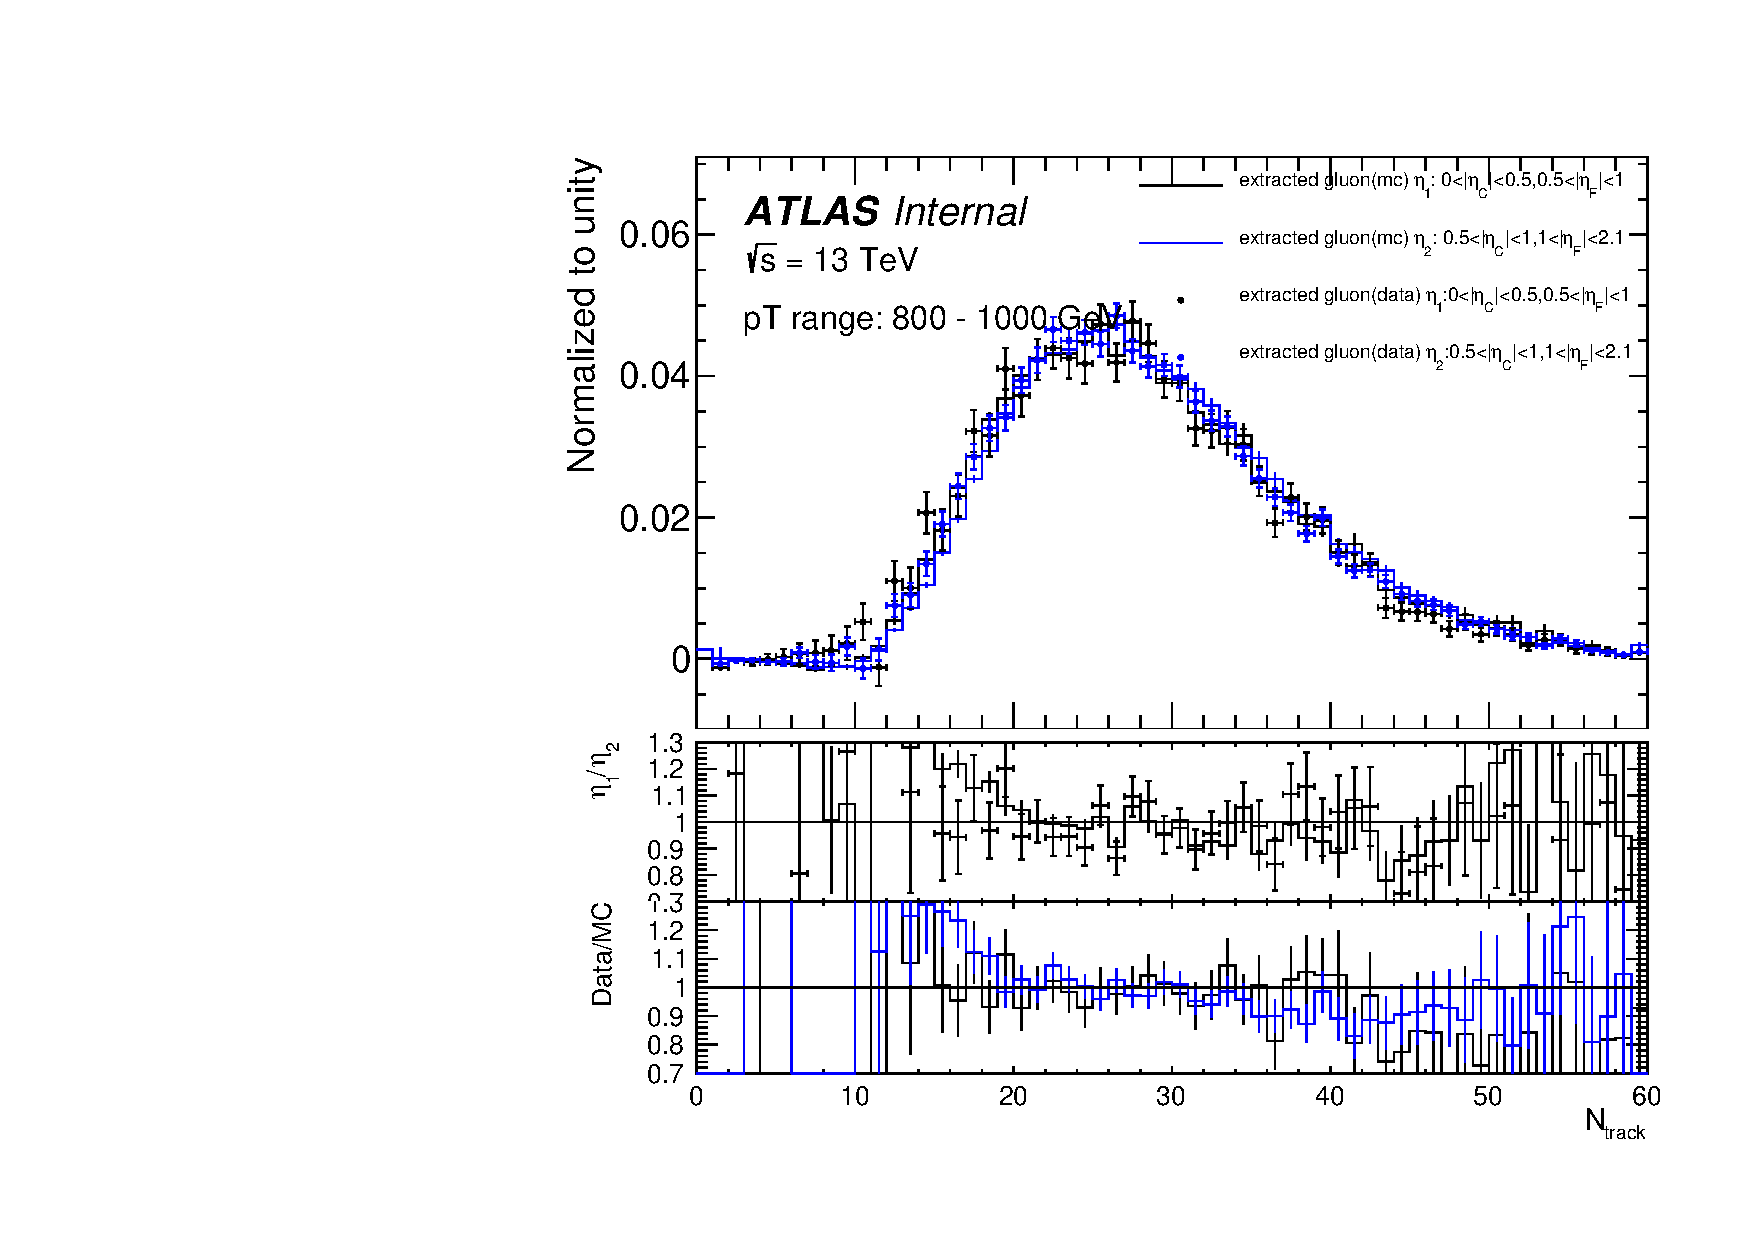
\includegraphics[width=0.45\textwidth]{fig/Method1/pythia/eta/extracted/plots_ntrk/gluon_800_Quark_pythia_ntrk_compare_0-0.5_0.5-1_0.5-1_1-2.1.pdf}}  \\
%	\caption[]{
%	  The $\ntrk$  distributions in 0 < $\mid\eta_{C}\mid$ < 0.5,0.5 < $\mid\eta_{F}\mid$ < 1 and in 0.5 < $\mid\eta_{C}\mid$ < 1,1 < $\mid\eta_{F}\mid$ < 2.1 of pure quark jets \subref{fig:QG-pythia-NtrkDataQa} \subref{fig:QG-pythia-NtrkDataQb} and  gluon jets \subref{fig:QG-pythia-NtrkDataGa} \subref{fig:QG-pythia-NtrkDataGb}  in 500-600GeV(top) and 800-1000GeV(bottom) by \pythia8. % 
%		extracted by the matrix method from the data and MC. %
%		Solid-line histograms show the distributions extracted by MC and dot histograms show the distributions extracted by Data.
%		A bottom panel in each figure shows the ratio of the extracted data to the extracted MC by the matrix method. %
%	In the top and bottom panel , black histograms are from 0 < $\mid\eta_{C}\mid$ < 0.5, 0.5 < $\mid\eta_{F}\mid$ < 1 and blue histograms are from  0.5 < $\mid\eta_{C}\mid$ < 1,1 < $\mid\eta_{F}\mid$ < 2.1. %
%	In the top and middle panel , solid-line and dot histograms show the Ntrk distributions in the extracted MC and extracted Data, respectively. %
%		\label{fig:QG-pythia-etabin-ntrk-Pythia}
%	}
%\end{figure}
%
%\begin{figure}[htb]
%	\centering
%	\subfloat[$Quark: 500<\pt<600\GeV$~(\pythia8)]{\label{fig:QG-pythia-BDTDataQa}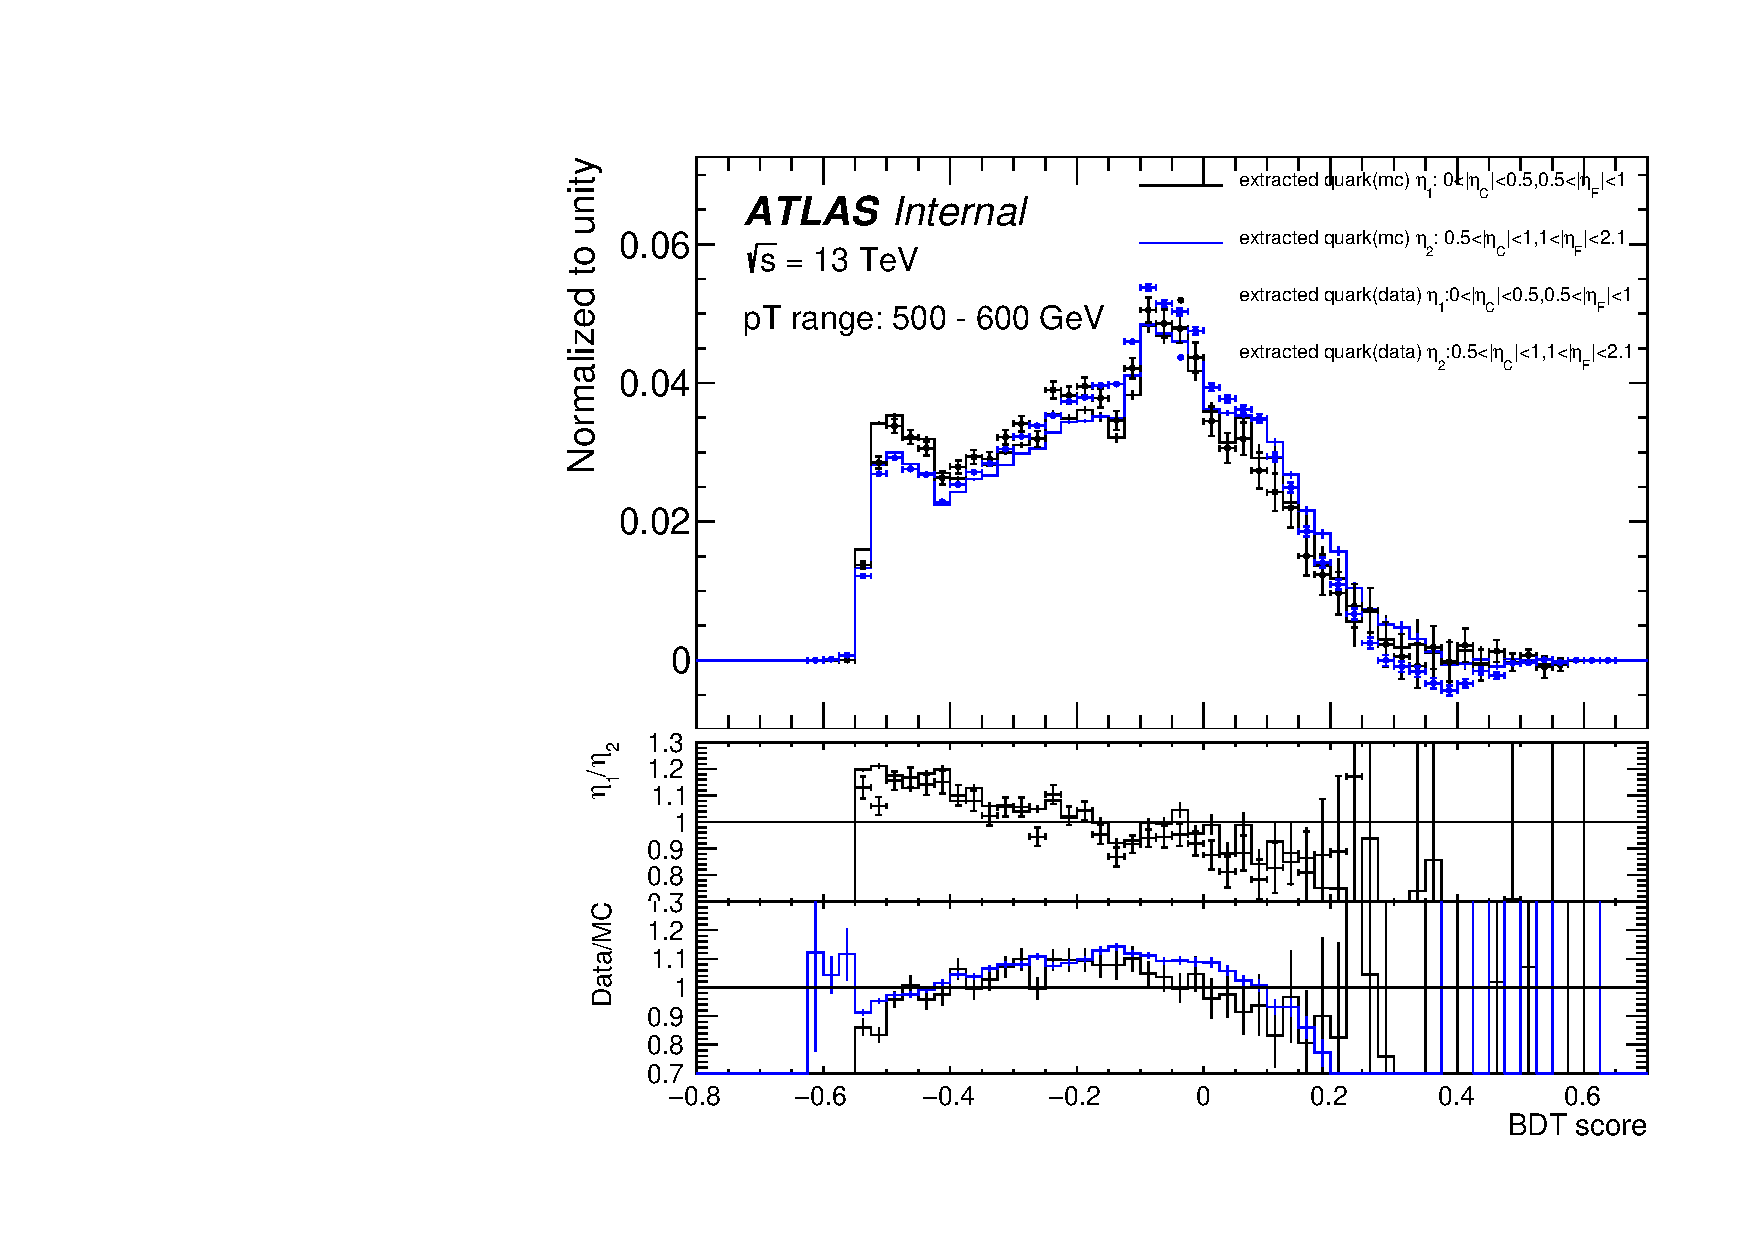
\includegraphics[width=0.45\textwidth]{fig/Method1/pythia/eta/extracted/plots_bdt/quark_500_Quark_pythia_bdt_compare_0-0.5_0.5-1_0.5-1_1-2.1.pdf}} \quad
%	\subfloat[$Gluon: 500<\pt<600\GeV$~(\pythia8)]{\label{fig:QG-pythia-BDTDataGa}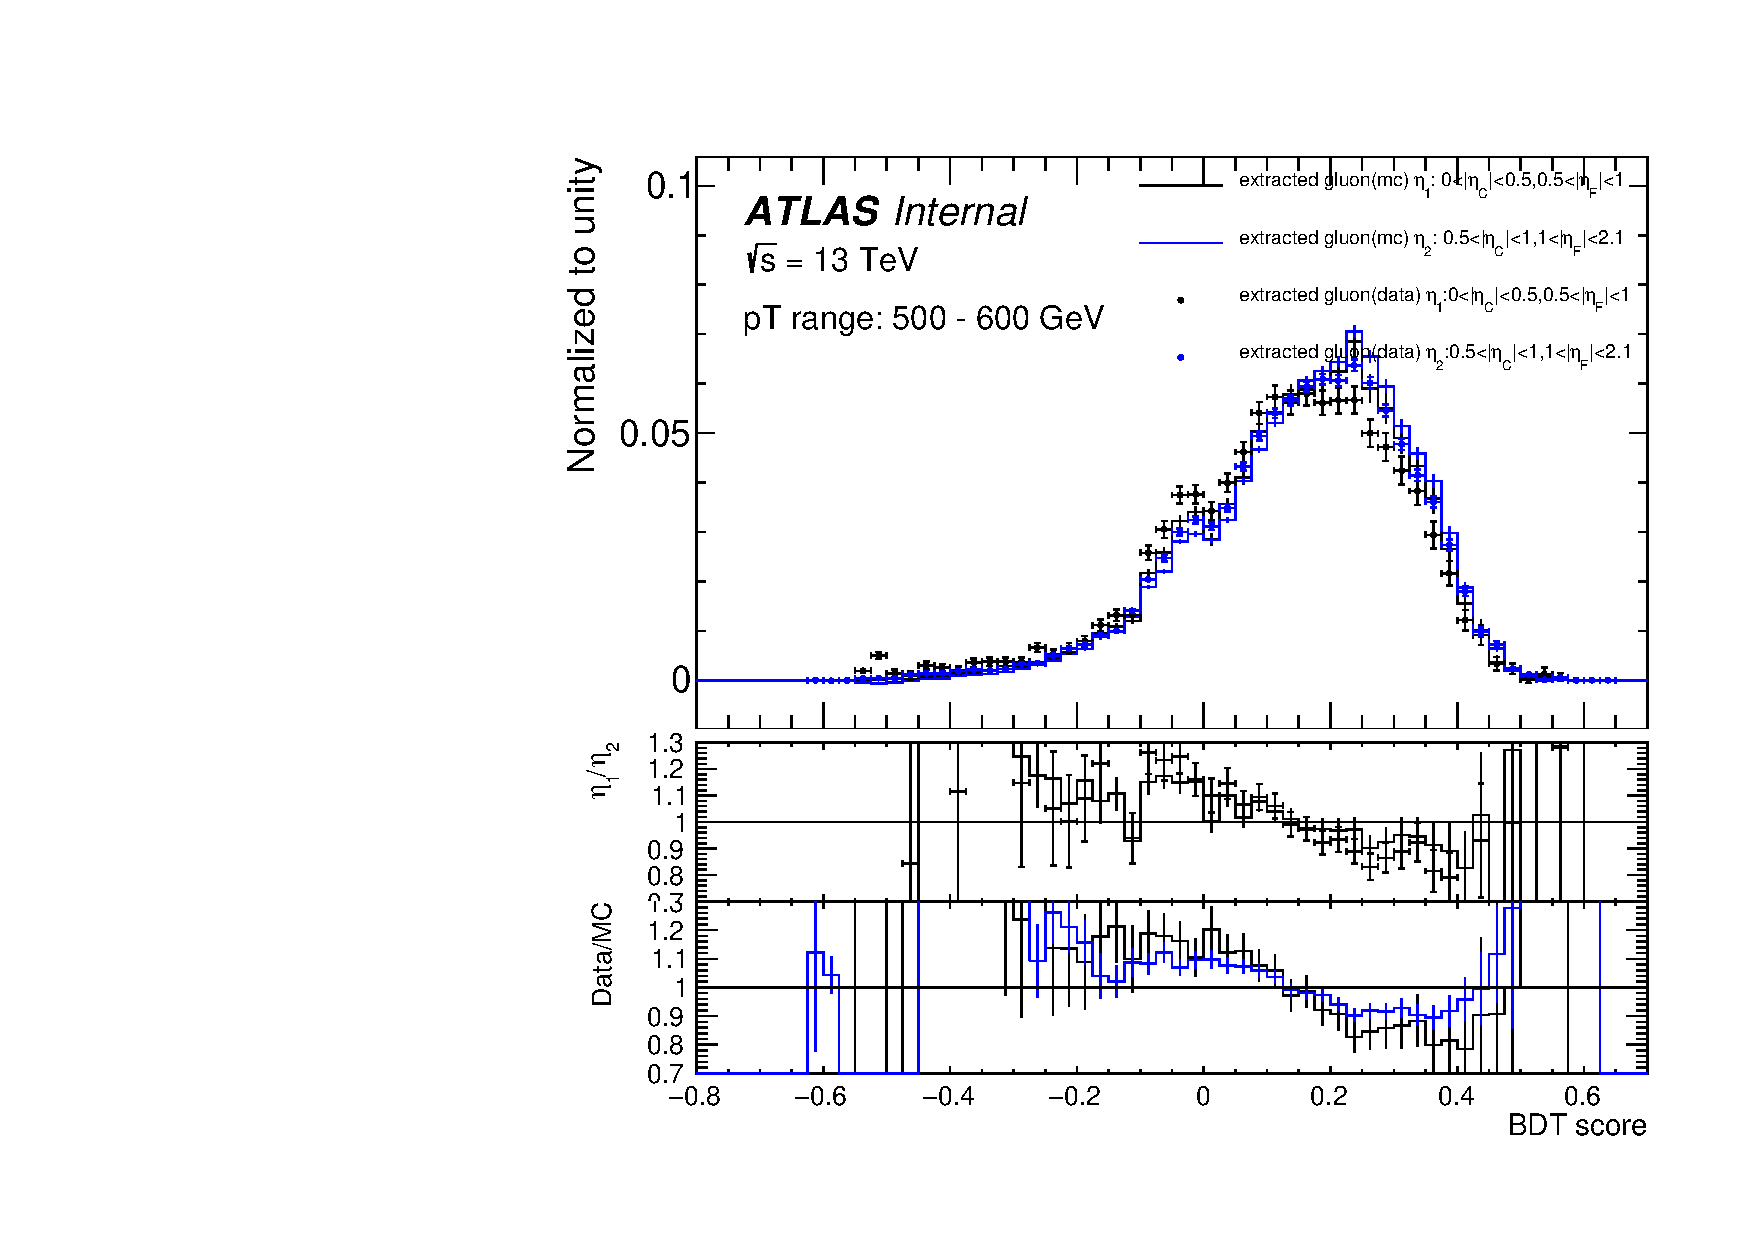
\includegraphics[width=0.45\textwidth]{fig/Method1/pythia/eta/extracted/plots_bdt/gluon_500_Quark_pythia_bdt_compare_0-0.5_0.5-1_0.5-1_1-2.1.pdf}}  \\
%	\subfloat[$Quark: 800<\pt<1000\GeV$~(\pythia8)]{\label{fig:QG-pythia-BDTDataQb}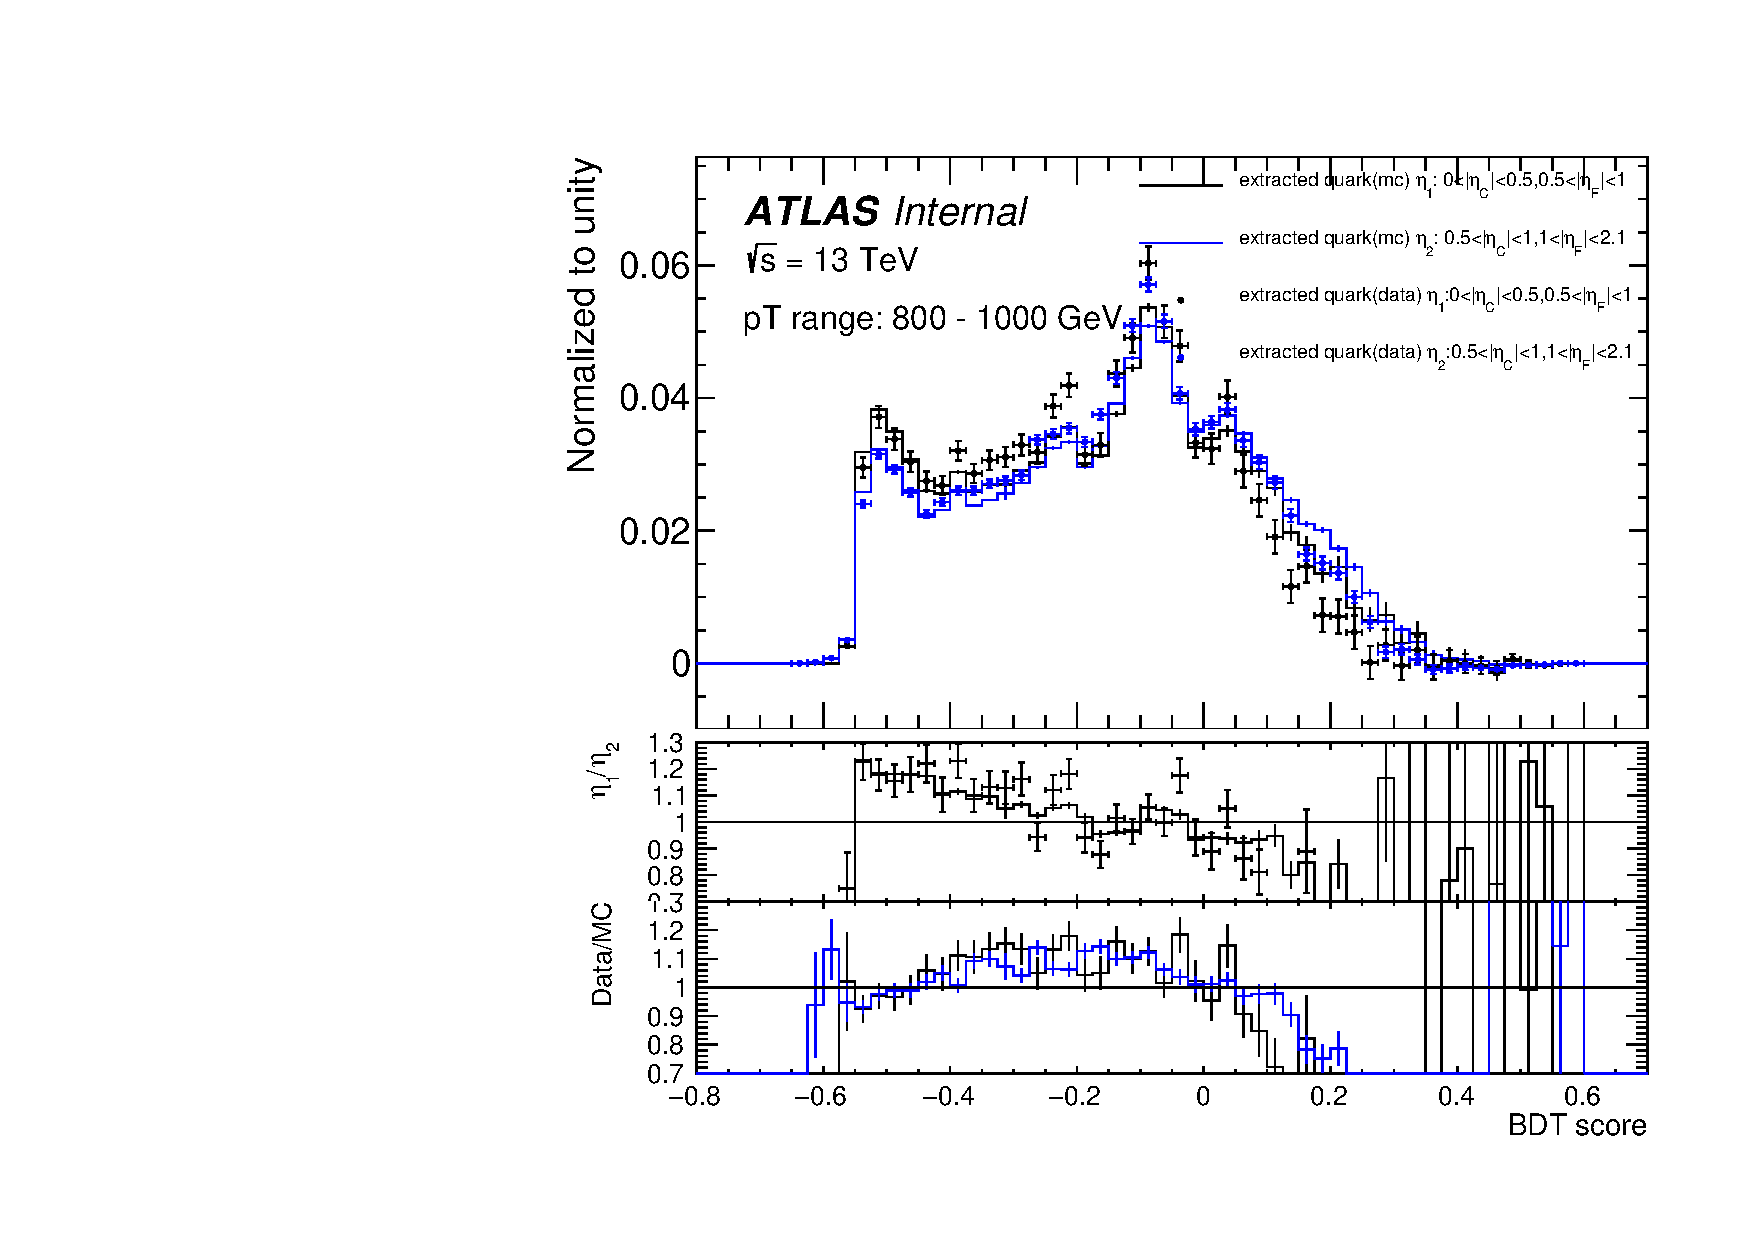
\includegraphics[width=0.45\textwidth]{fig/Method1/pythia/eta/extracted/plots_bdt/quark_800_Quark_pythia_bdt_compare_0-0.5_0.5-1_0.5-1_1-2.1.pdf}} \quad
%	\subfloat[$Gluon: 800<\pt<1000\GeV$~(\pythia8)]{\label{fig:QG-pythia-BDTDataGb}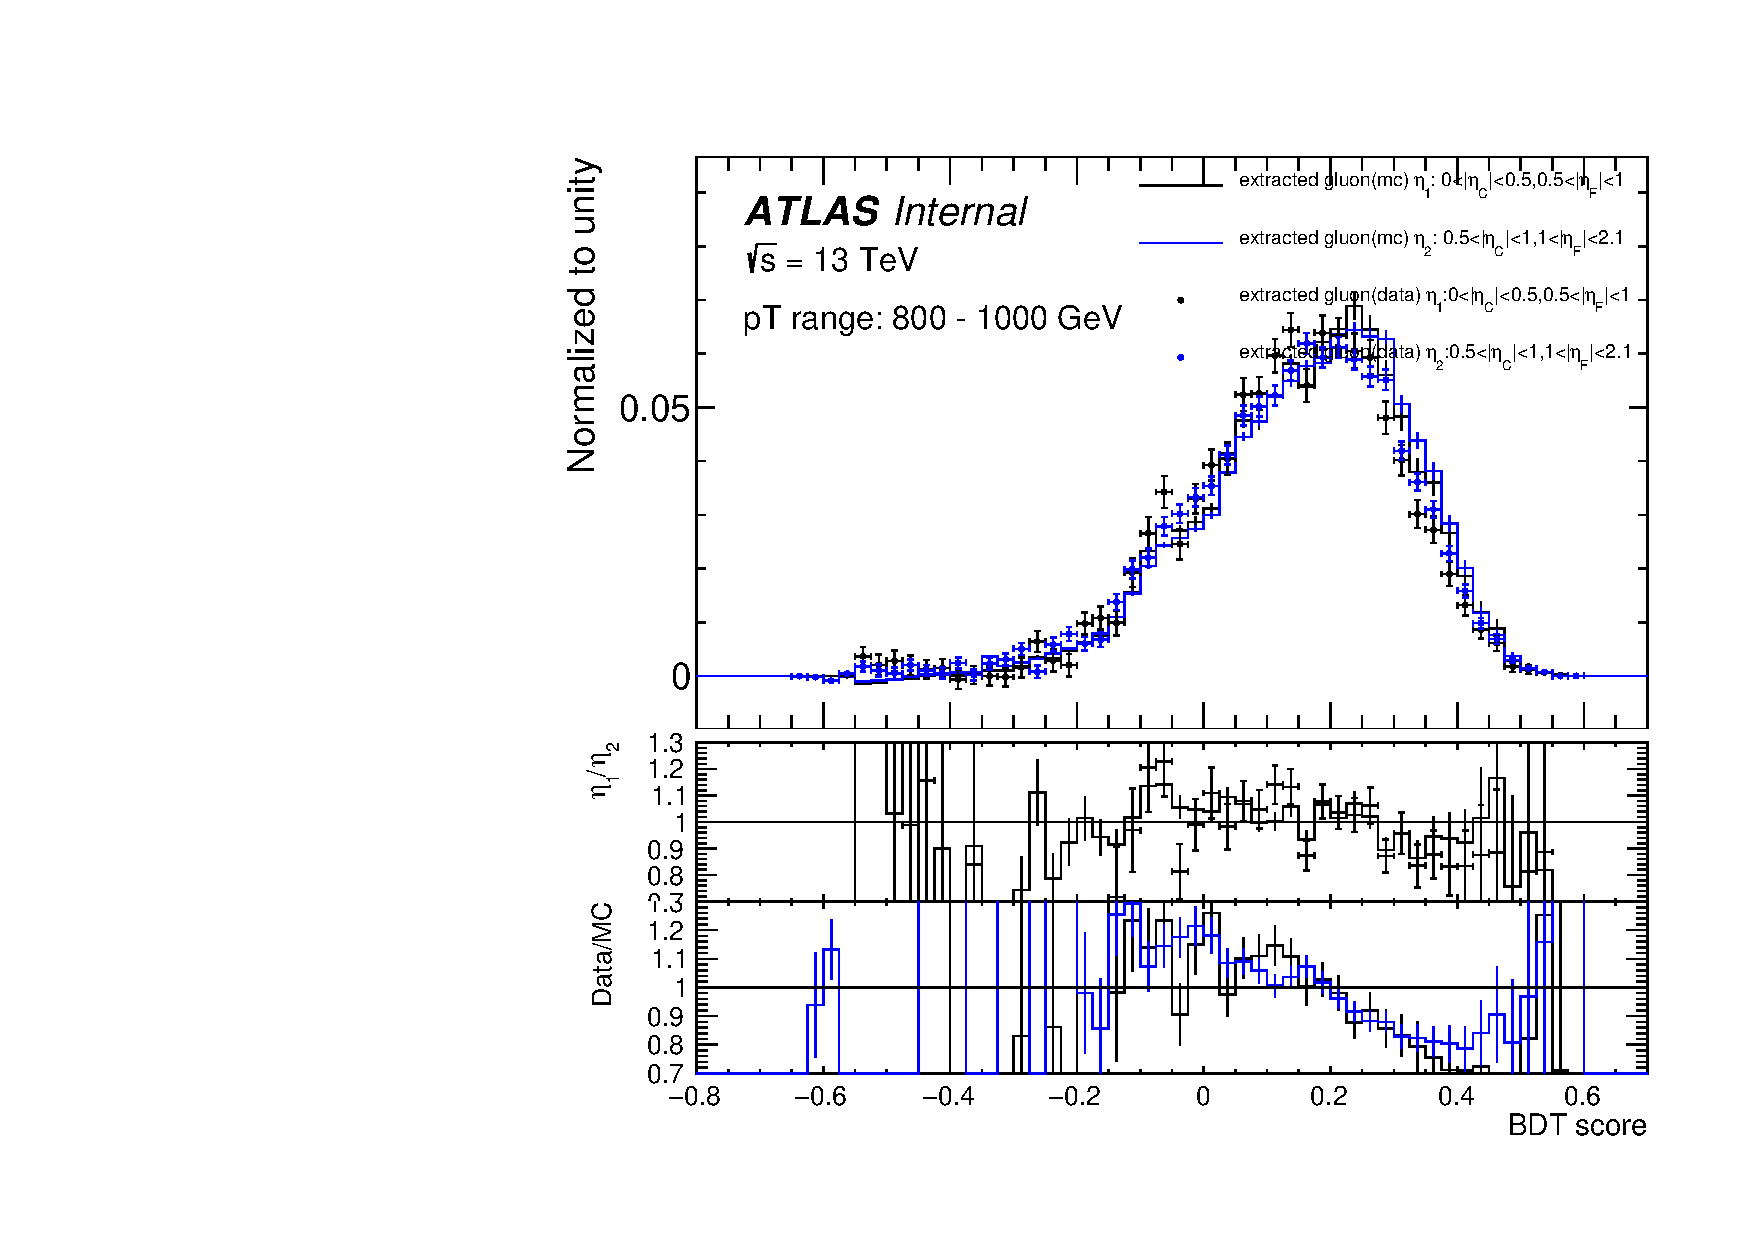
\includegraphics[width=0.45\textwidth]{fig/Method1/pythia/eta/extracted/plots_bdt/gluon_800_Quark_pythia_bdt_compare_0-0.5_0.5-1_0.5-1_1-2.1.pdf}}  \\
%	\caption[]{
%	  The BDT distributions in 0 < $\mid\eta_{C}\mid$ < 0.5,0.5 < $\mid\eta_{F}\mid$ < 1 and in 0.5 < $\mid\eta_{C}\mid$ < 1,1 < $\mid\eta_{F}\mid$ < 2.1 of pure quark jets \subref{fig:QG-pythia-BDTDataQa} \subref{fig:QG-pythia-BDTDataQb} and  gluon jets \subref{fig:QG-pythia-BDTDataGa} \subref{fig:QG-pythia-BDTDataGb}  in 500-600GeV(top) and 800-1000GeV(bottom) by \pythia8. % 
%		extracted by the matrix method from the data and MC. %
%	In the top and bottom panel , black histograms are from 0 < $\mid\eta_{C}\mid$ < 0.5,0.5 < $\mid\eta_{F}\mid$ < 1 and blue histograms are from  0.5 < $\mid\eta_{C}\mid$ < 1,1 < $\mid\eta_{F}\mid$ < 2.1. %
%	In the top and middle panel , solid-line and dot histograms show the BDT distributions in the extracted MC and extracted Data, respectively. %
%		\label{fig:QG-pythia-etabin-BDT-Pythia}
%	}
%\end{figure}
%
%\begin{figure}[htb]
%	\centering
%	\subfloat[Quark,Working Point:50\%~(\pythia8)]{\label{fig:QG-pythia-NtrkDataQWP}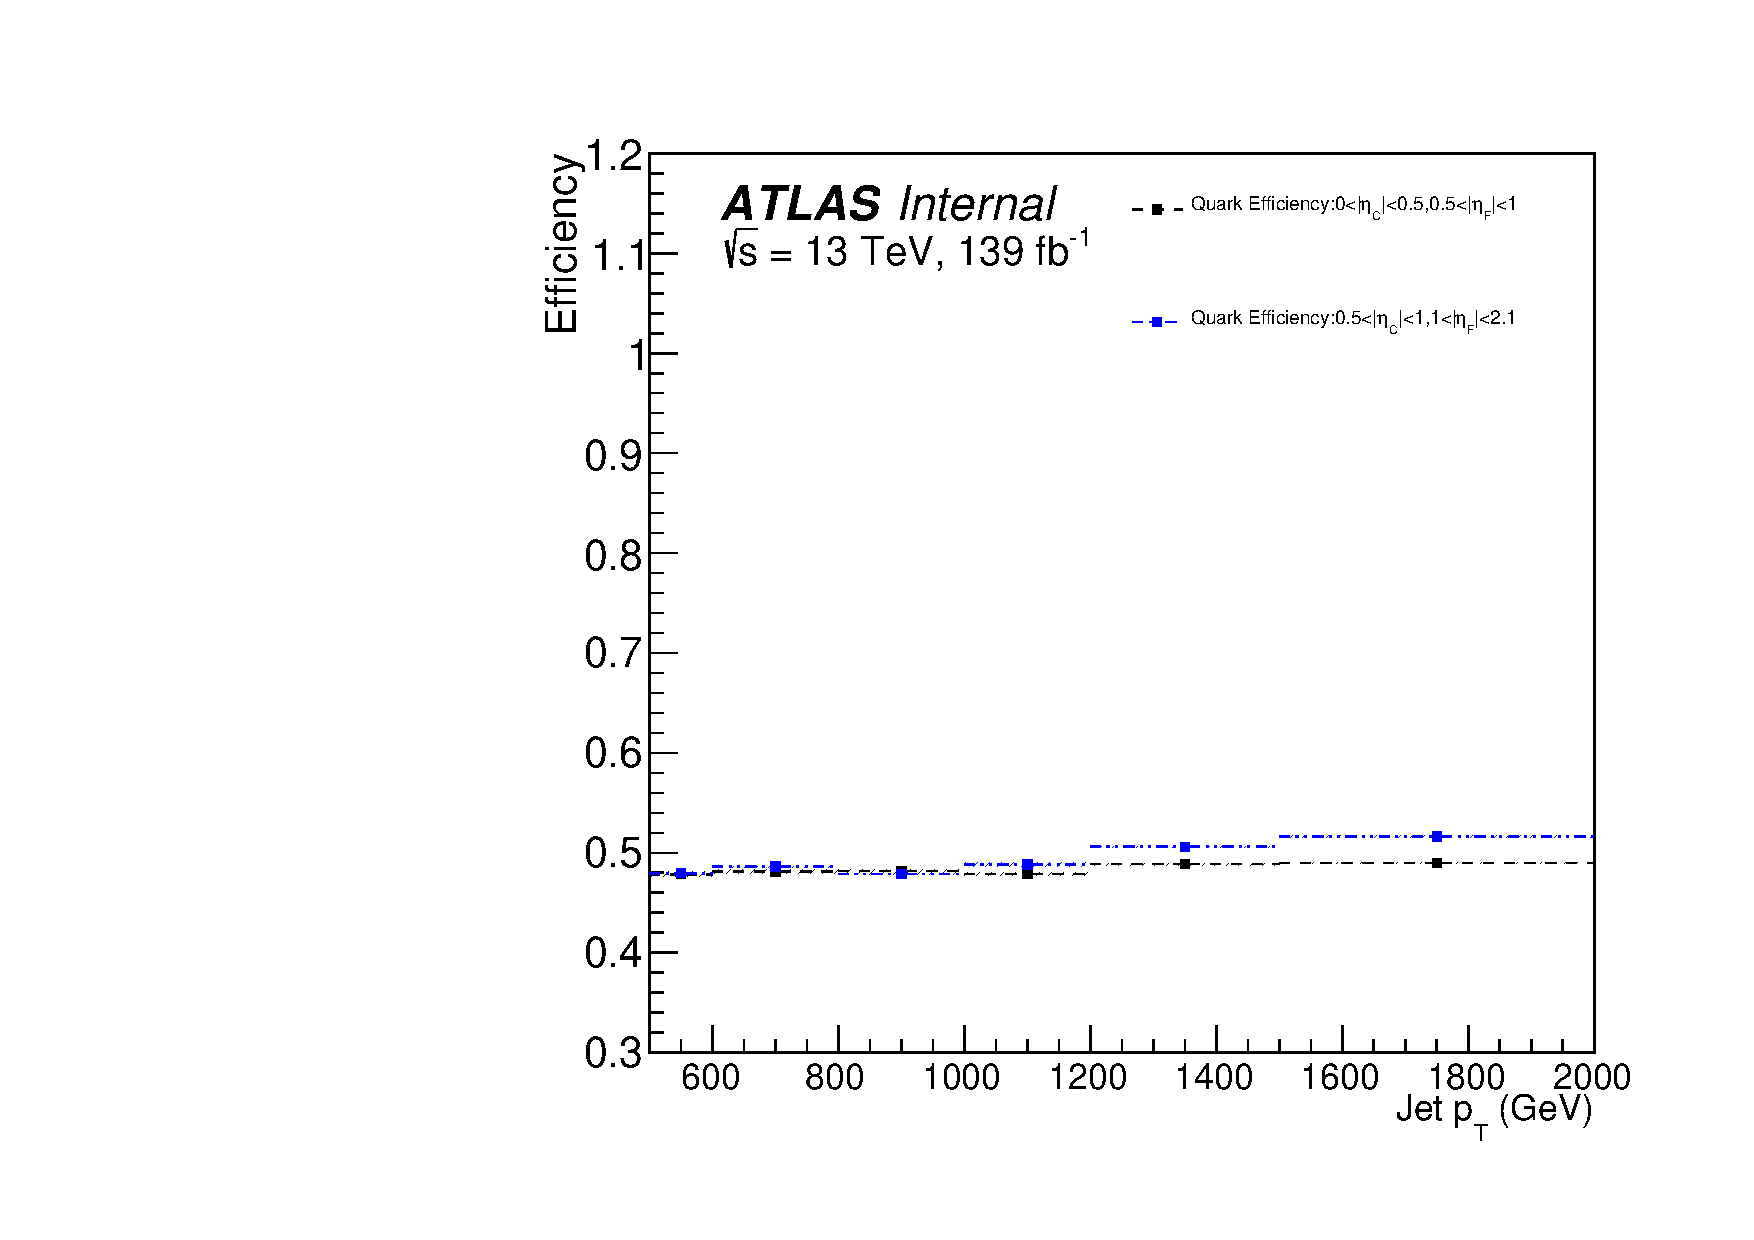
\includegraphics[width=0.45\textwidth]{fig/Method1/pythia/eta/working-point-SF-compare/0-0.5_0.5-1_0.5-1_1-2.1-Quark-WP-0.5-ntrk.pdf}} \quad
%	\subfloat[Quark,Working Point:50\%~(\pythia8)]{\label{fig:QG-pythia-NtrkDataQSF}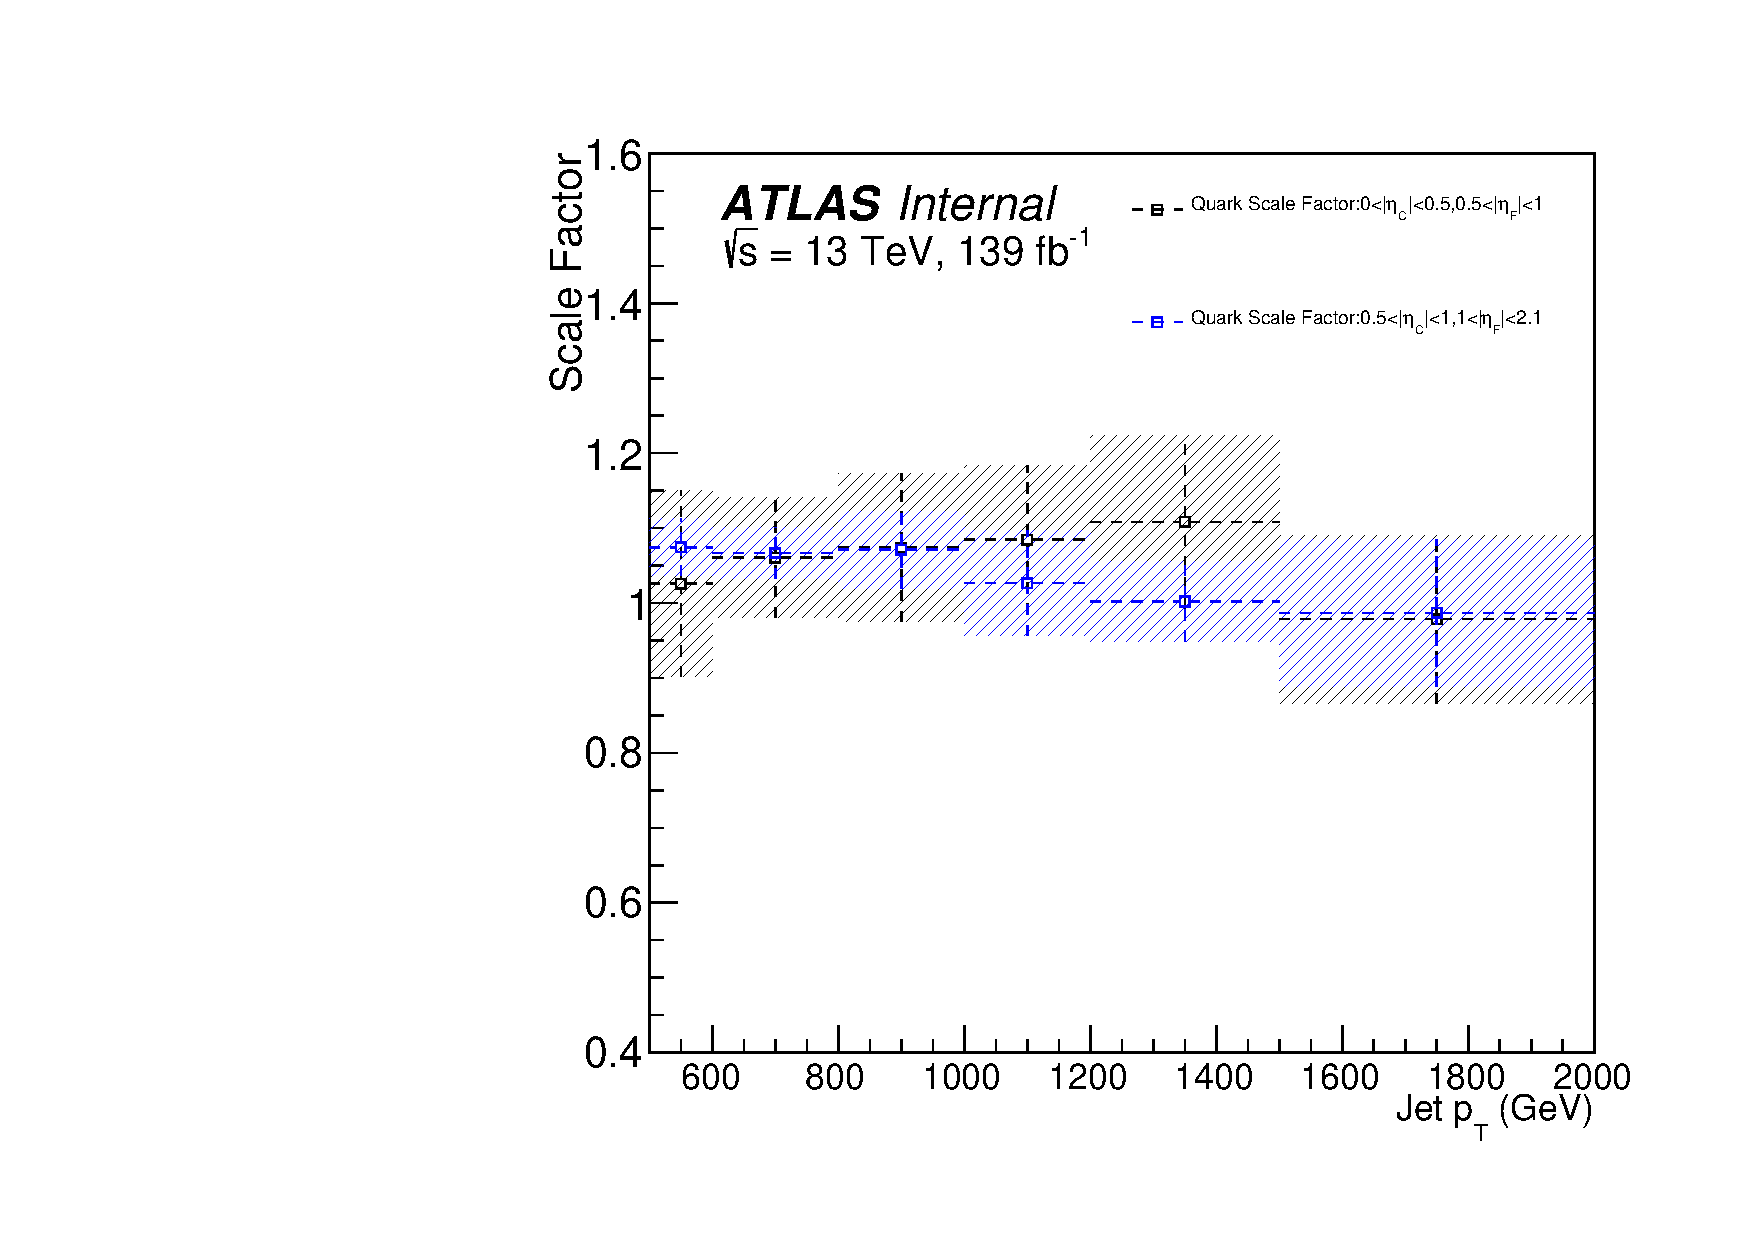
\includegraphics[width=0.45\textwidth]{fig/Method1/pythia/eta/working-point-SF-compare/0-0.5_0.5-1_0.5-1_1-2.1-Quark-SF-0.5-ntrk.pdf}}\\
%	\subfloat[Gluon,Working Point:50\%~(\pythia8)]{\label{fig:QG-pythia-NtrkDataGWP}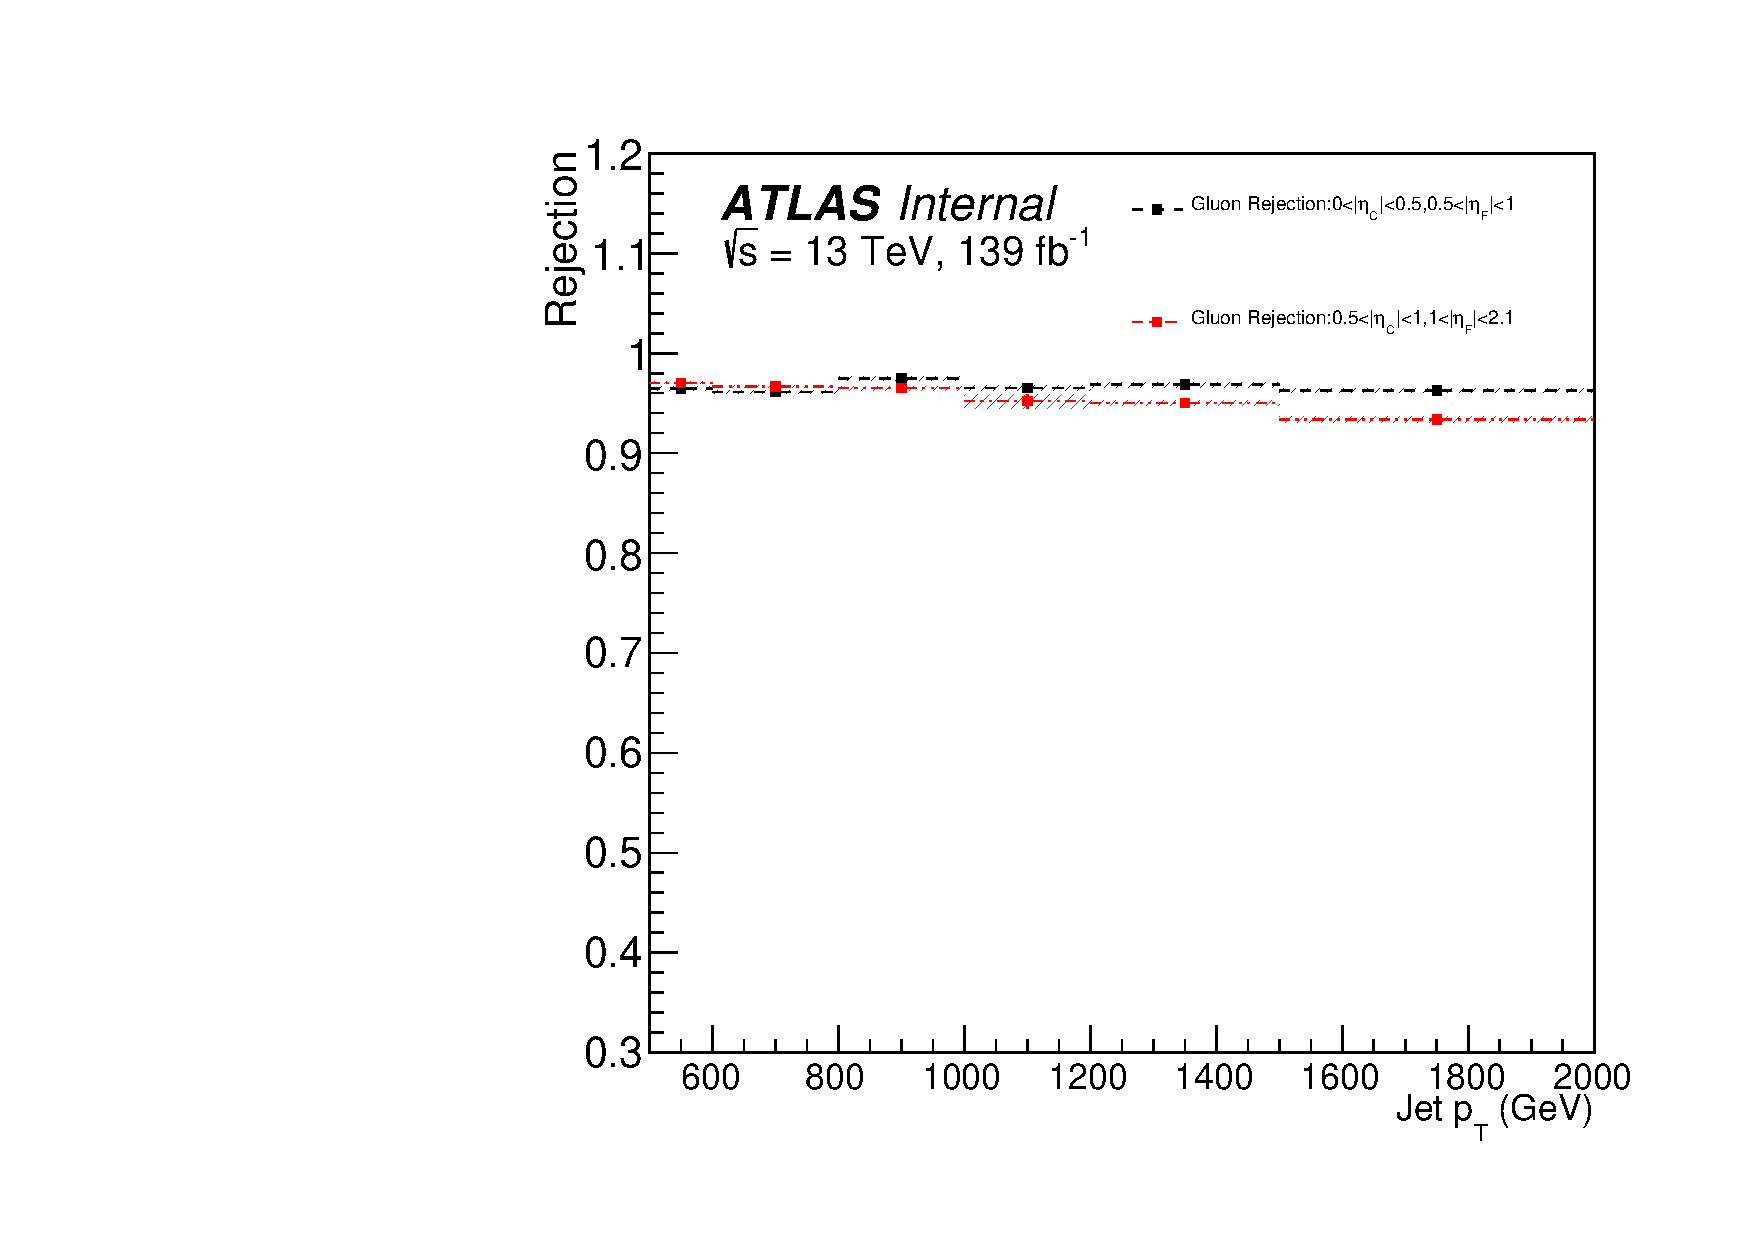
\includegraphics[width=0.45\textwidth]{fig/Method1/pythia/eta/working-point-SF-compare/0-0.5_0.5-1_0.5-1_1-2.1-Gluon-WP-0.5-ntrk.pdf}} \quad
%	\subfloat[Gluon,Working Point:50\%~(\pythia8)]{\label{fig:QG-pythia-NtrkDataGSF}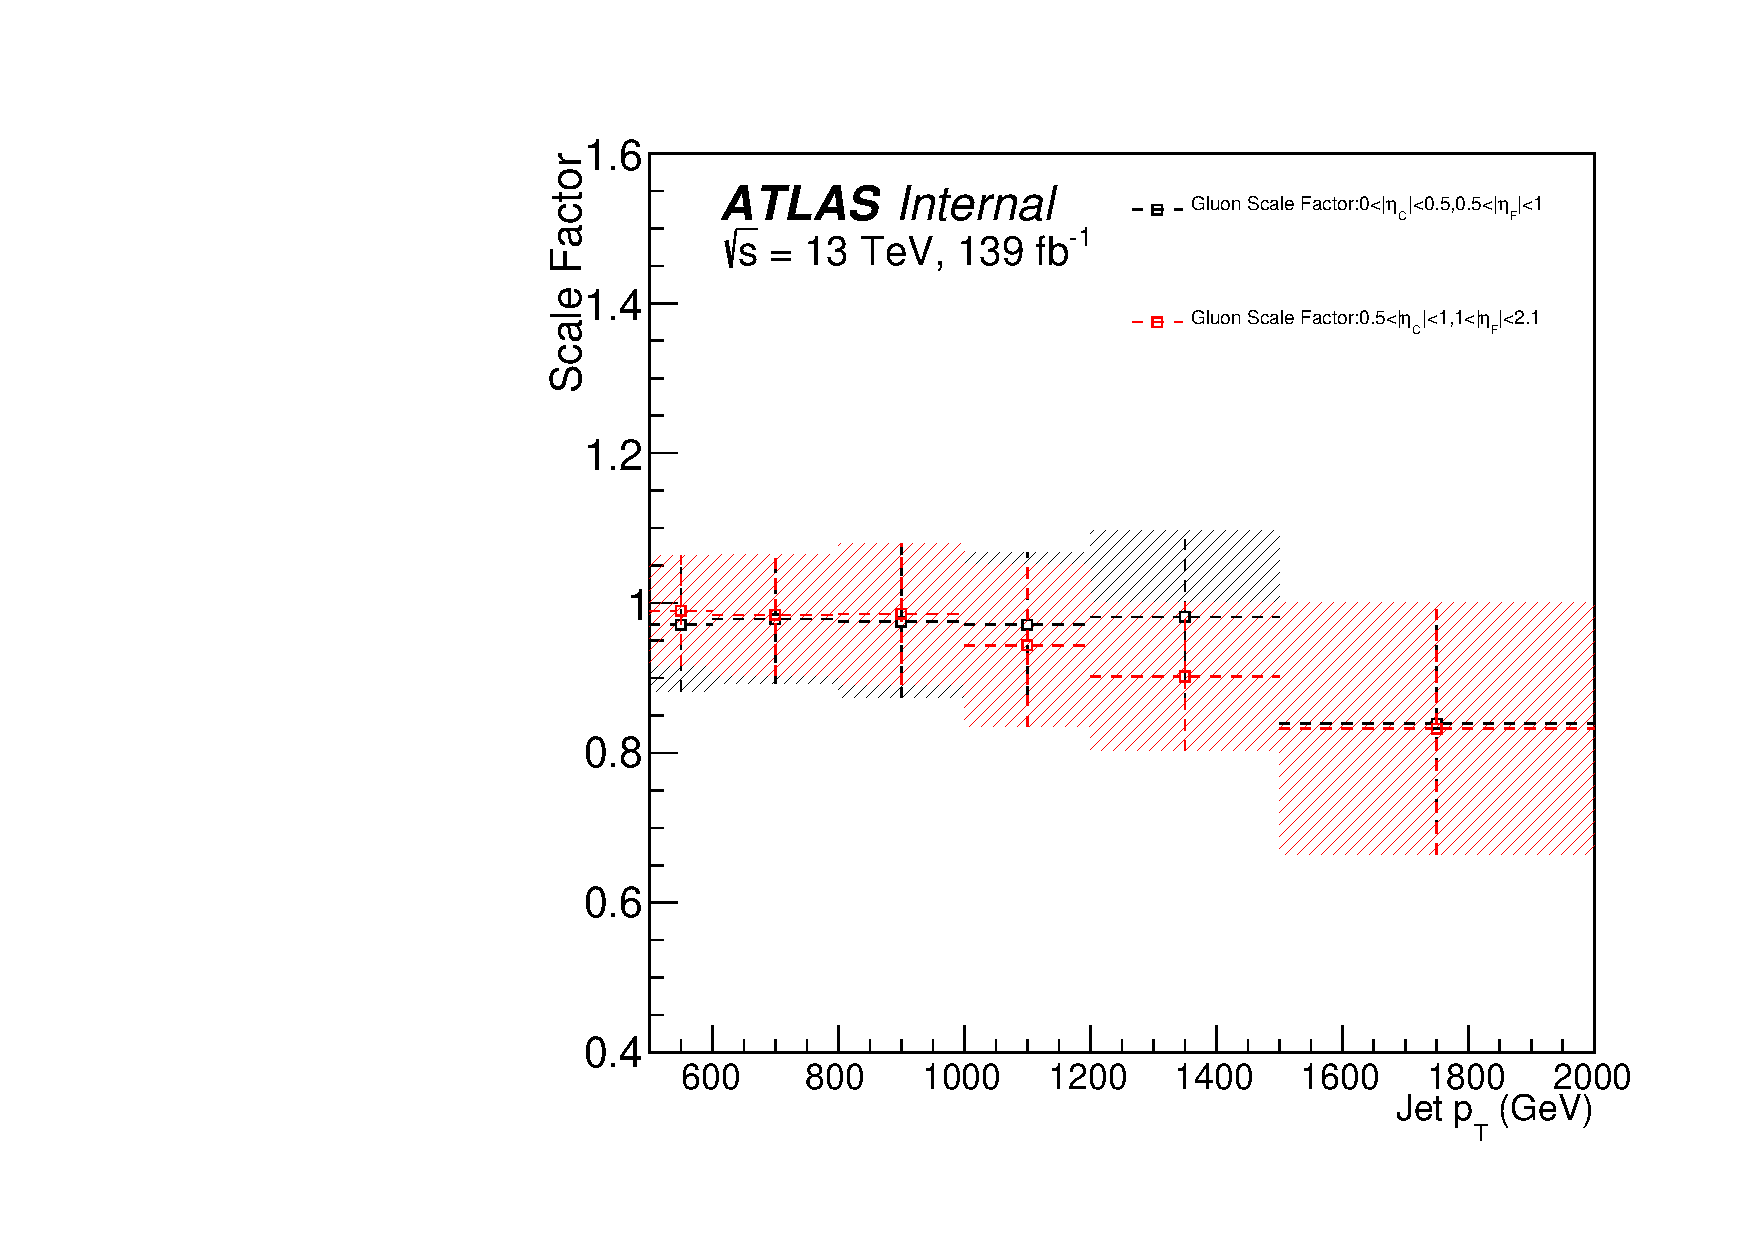
\includegraphics[width=0.45\textwidth]{fig/Method1/pythia/eta/working-point-SF-compare/0-0.5_0.5-1_0.5-1_1-2.1-Gluon-SF-0.5-ntrk.pdf}}\\
%	\caption[]{
%	For 50$\%$ working point of \ntrk ,compare quark efficiency,gluon rejection and scale factors in 0<$\mid\eta_{C}\mid$<0.5,0.5<$\mid\eta_{F}\mid$<1 and in 0.5<$\mid\eta_{C}\mid$<1,1<$\mid\eta_{F}\mid$<2.1.%
%	The left plots are for quark efficiency and gluon rejection and the right plots are for scale factors. %
%	\subref{fig:QG-pythia-NtrkDataQWP}  \subref{fig:QG-pythia-NtrkDataQSF} are for quark distribution and \subref{fig:QG-pythia-NtrkDataGWP}  \subref{fig:QG-pythia-NtrkDataGSF} are for gluon distribution. %
% 	The error bars include the statistical uncertainty for quark efficiency and gluon factor and include statistical and parton shower modeling uncertainty for scale factors. %
%		\label{fig:QG-pythia-eta-Ntrk-5}
%	}
%\end{figure}
%
%\begin{figure}[htb]
%	\centering
%	\subfloat[Quark,Working Point:60\%~(\pythia8)]{\label{fig:QG-pythia-NtrkDataQWP}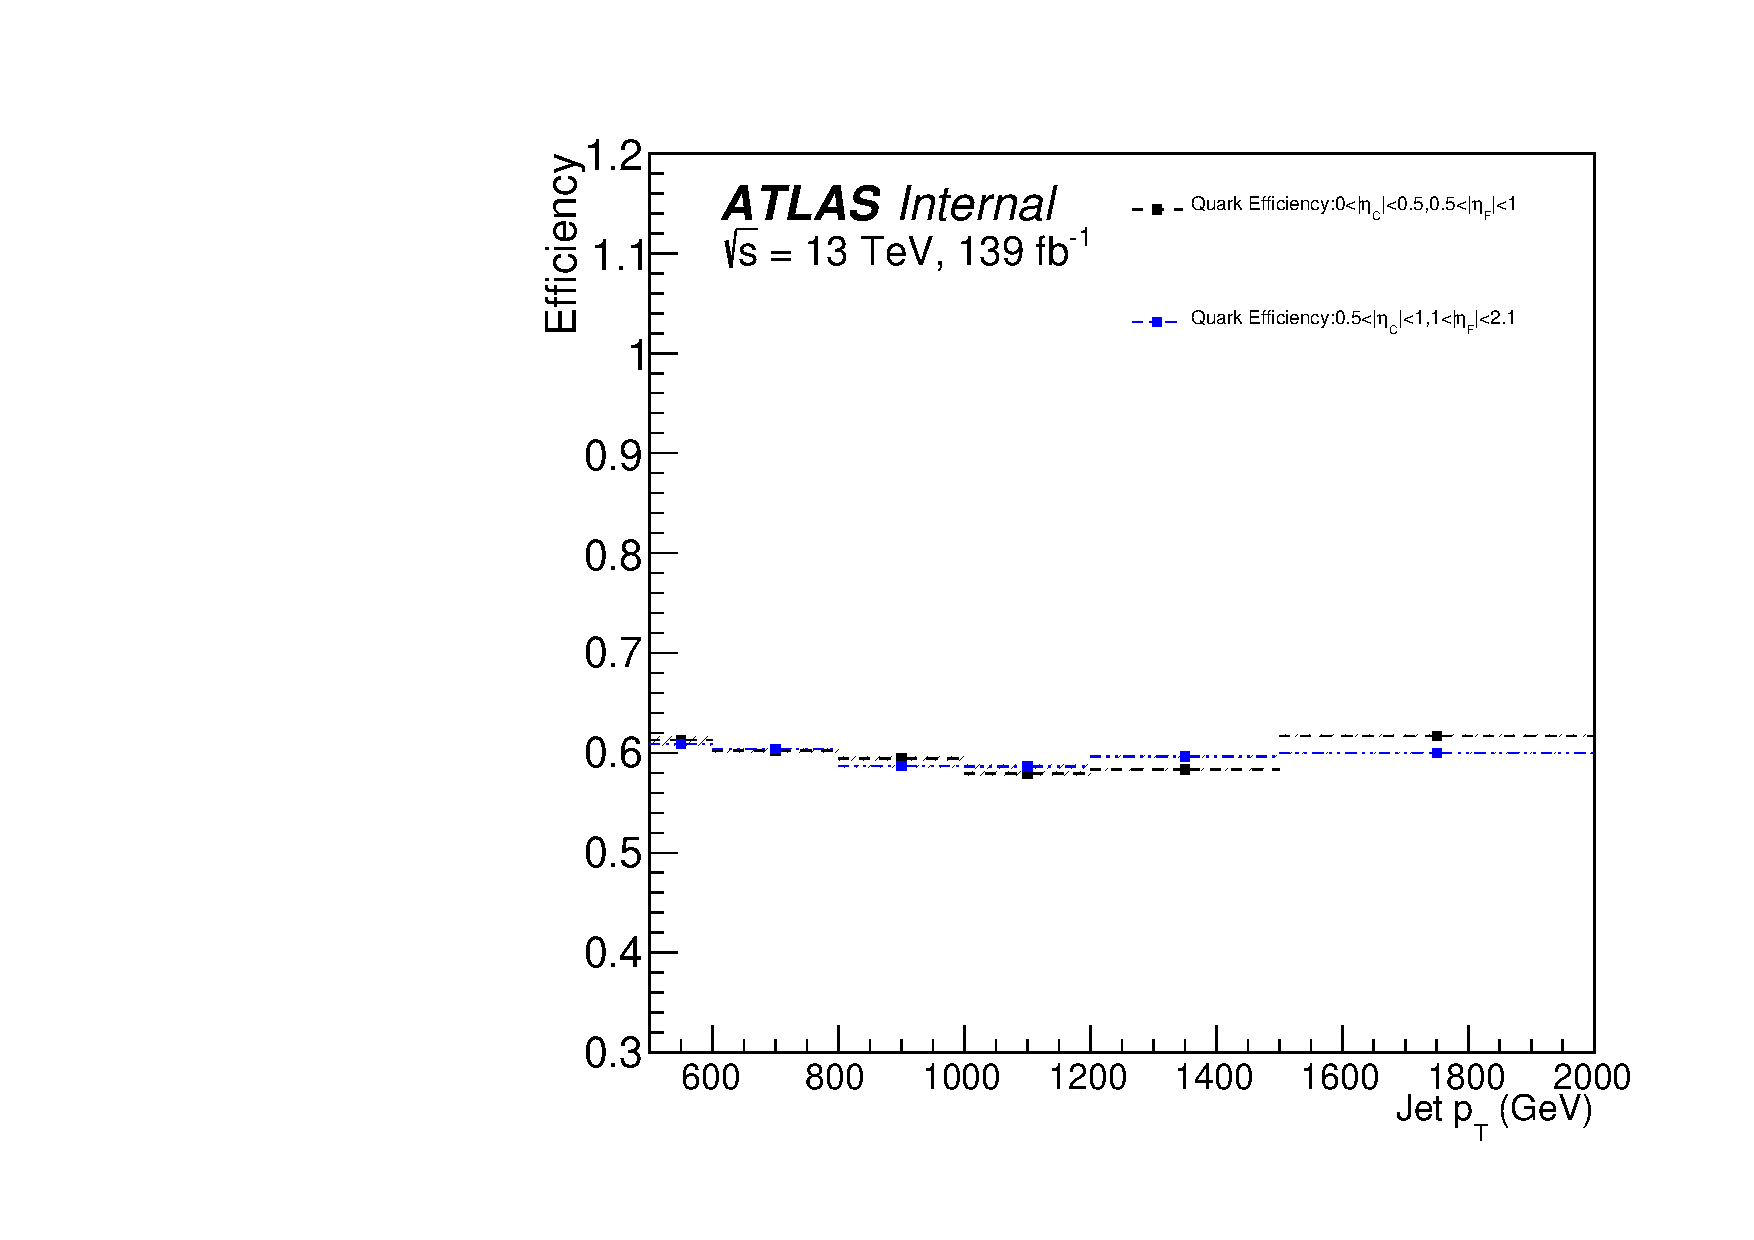
\includegraphics[width=0.45\textwidth]{fig/Method1/pythia/eta/working-point-SF-compare/0-0.5_0.5-1_0.5-1_1-2.1-Quark-WP-0.6-ntrk.pdf}} \quad
%	\subfloat[Quark,Working Point:60\%~(\pythia8)]{\label{fig:QG-pythia-NtrkDataQSF}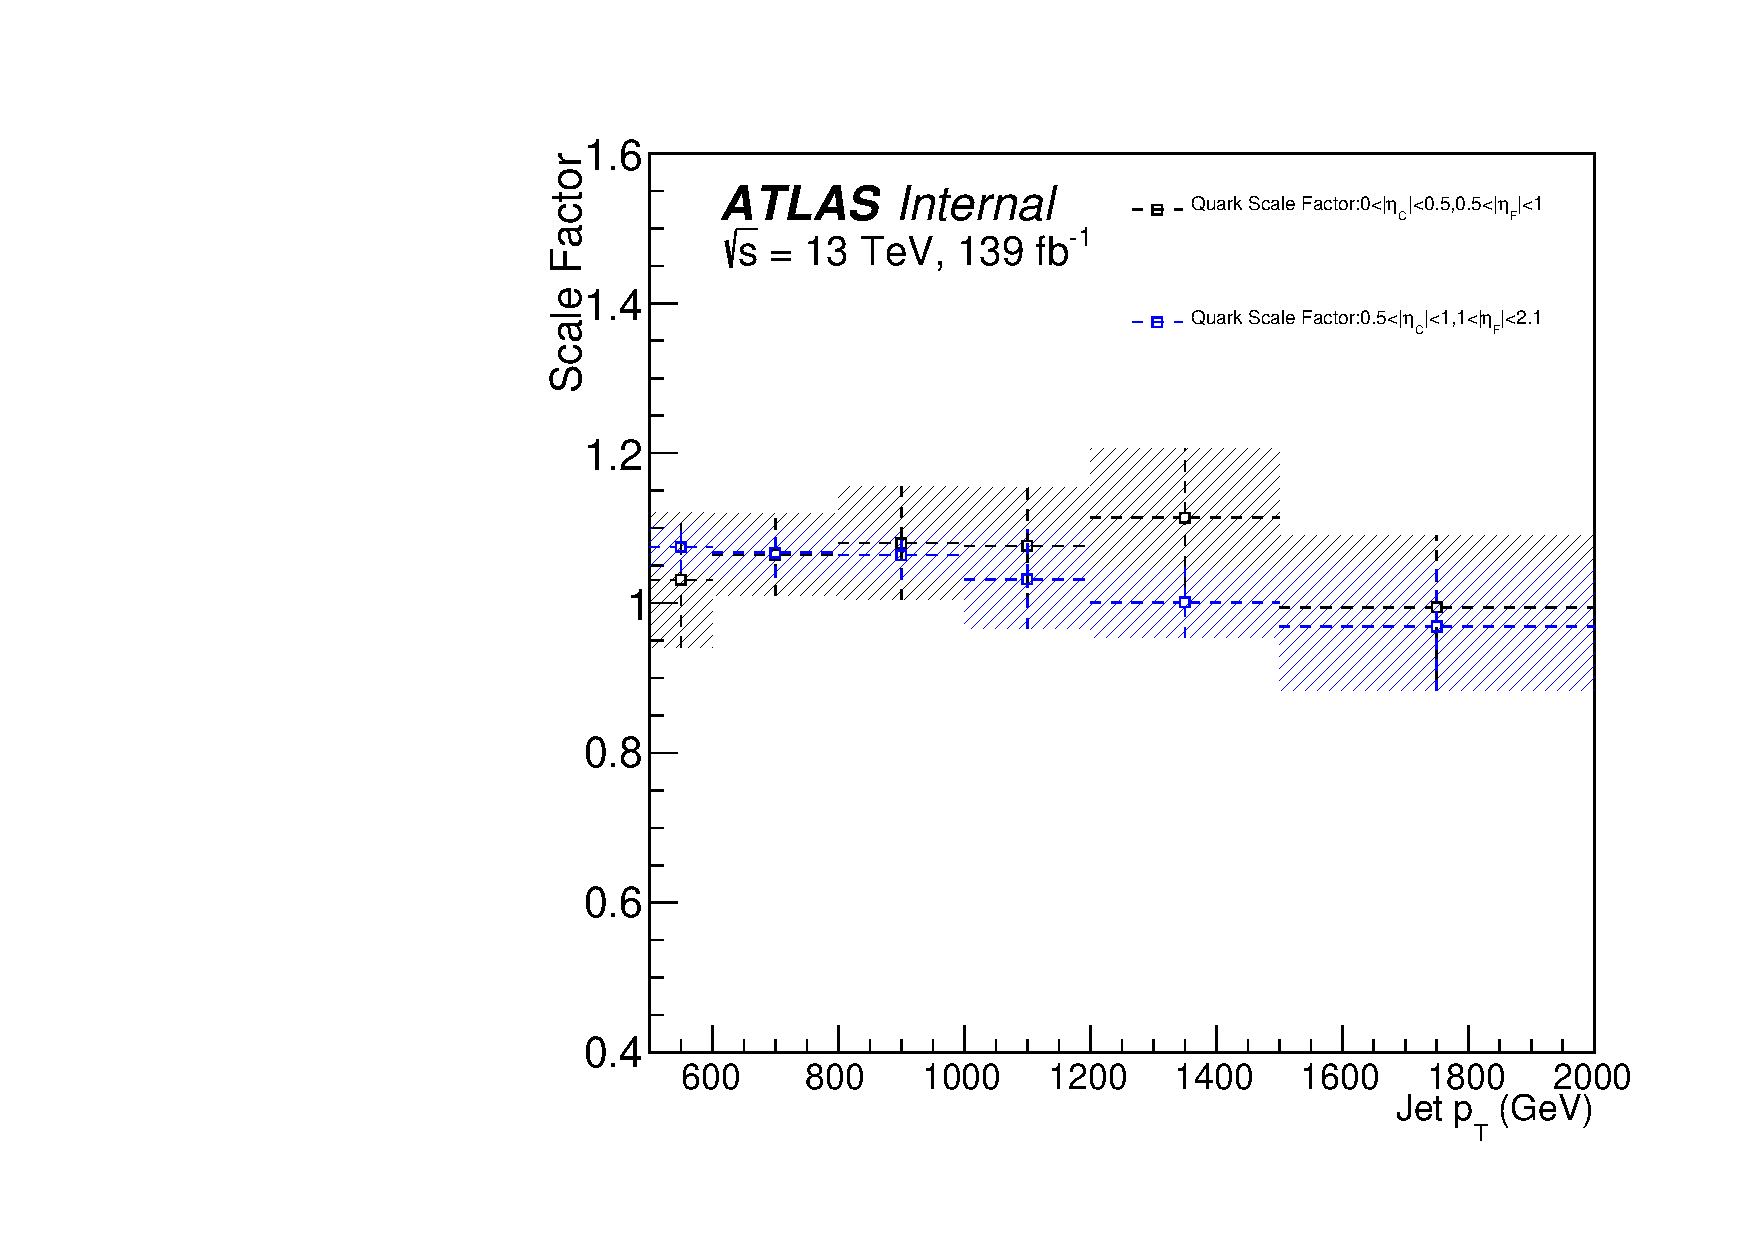
\includegraphics[width=0.45\textwidth]{fig/Method1/pythia/eta/working-point-SF-compare/0-0.5_0.5-1_0.5-1_1-2.1-Quark-SF-0.6-ntrk.pdf}}\\
%	\subfloat[Gluon,Working Point:60\%~(\pythia8)]{\label{fig:QG-pythia-NtrkDataGWP}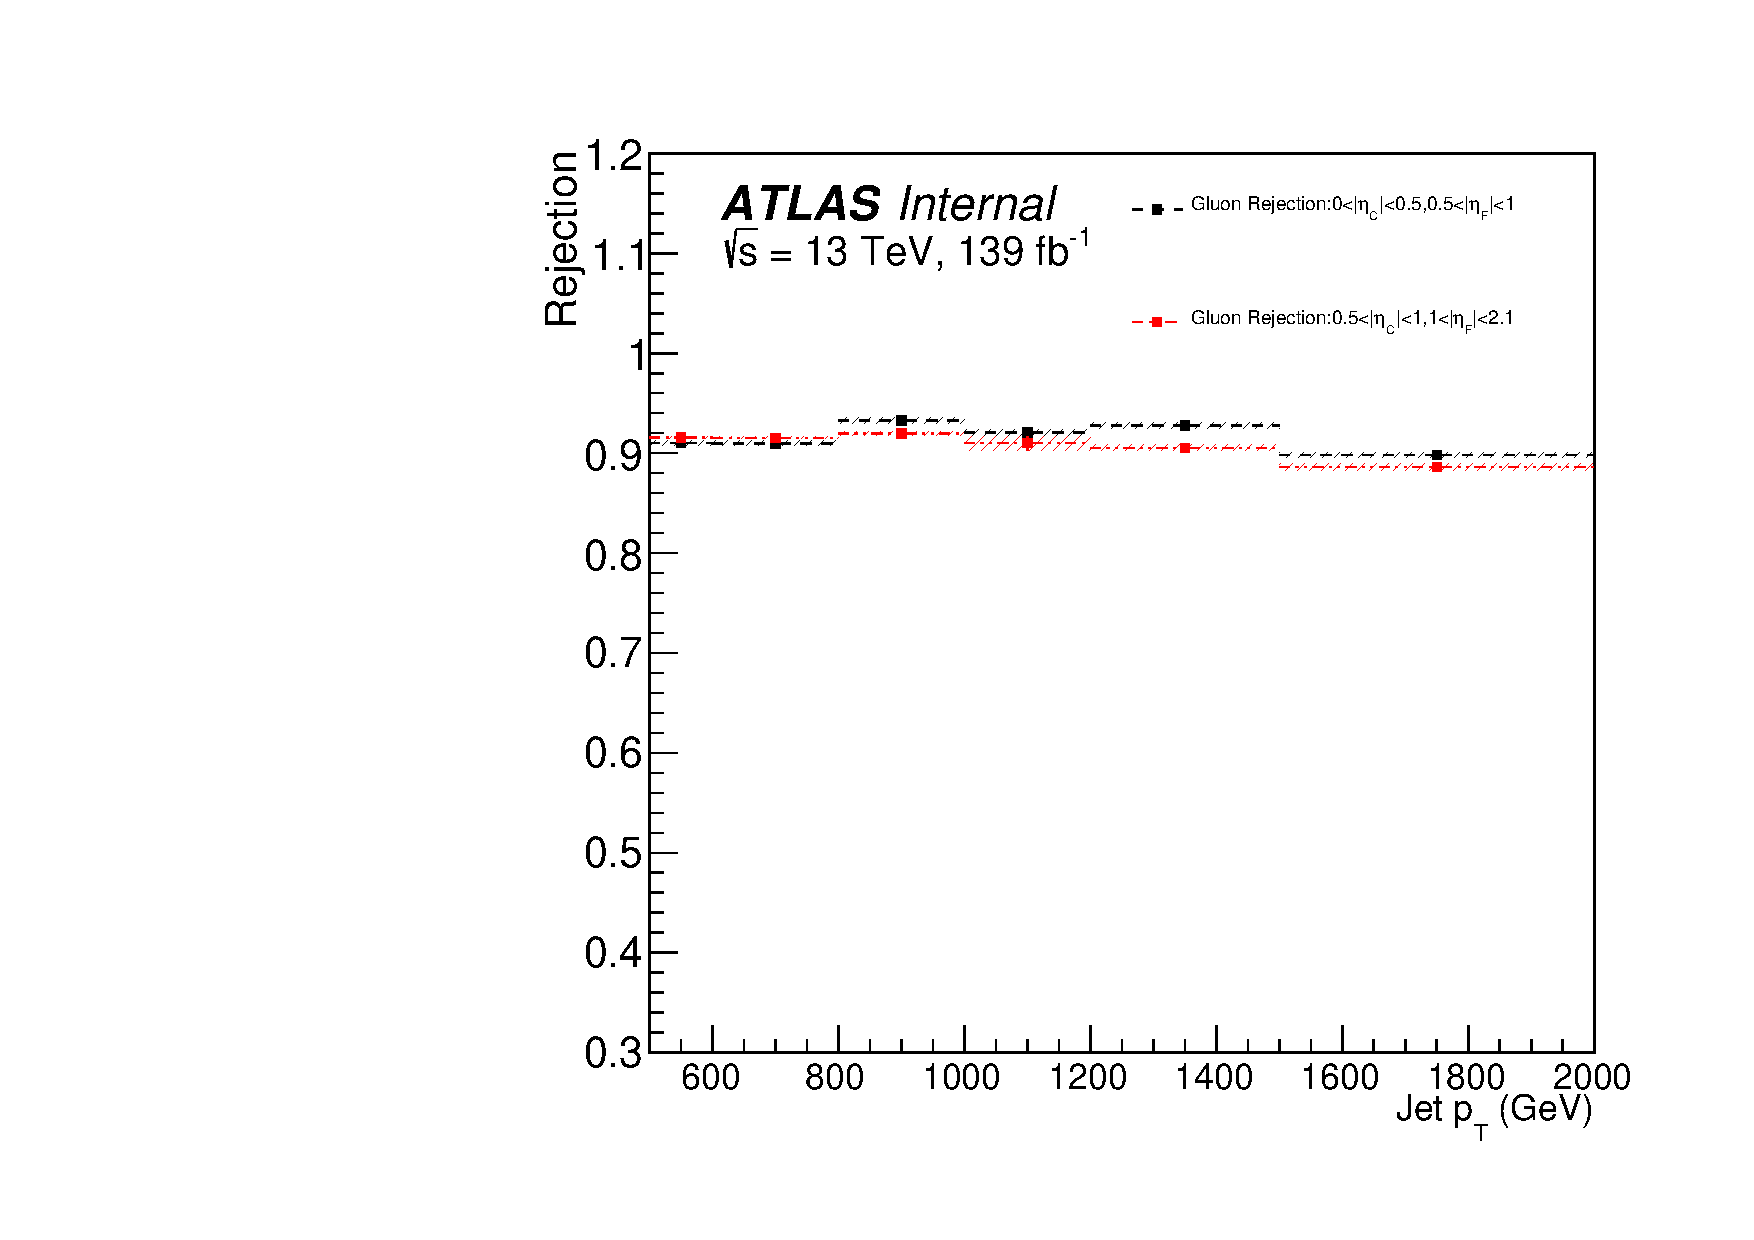
\includegraphics[width=0.45\textwidth]{fig/Method1/pythia/eta/working-point-SF-compare/0-0.5_0.5-1_0.5-1_1-2.1-Gluon-WP-0.6-ntrk.pdf}} \quad
%	\subfloat[Gluon,Working Point:60\%~(\pythia8)]{\label{fig:QG-pythia-NtrkDataGSF}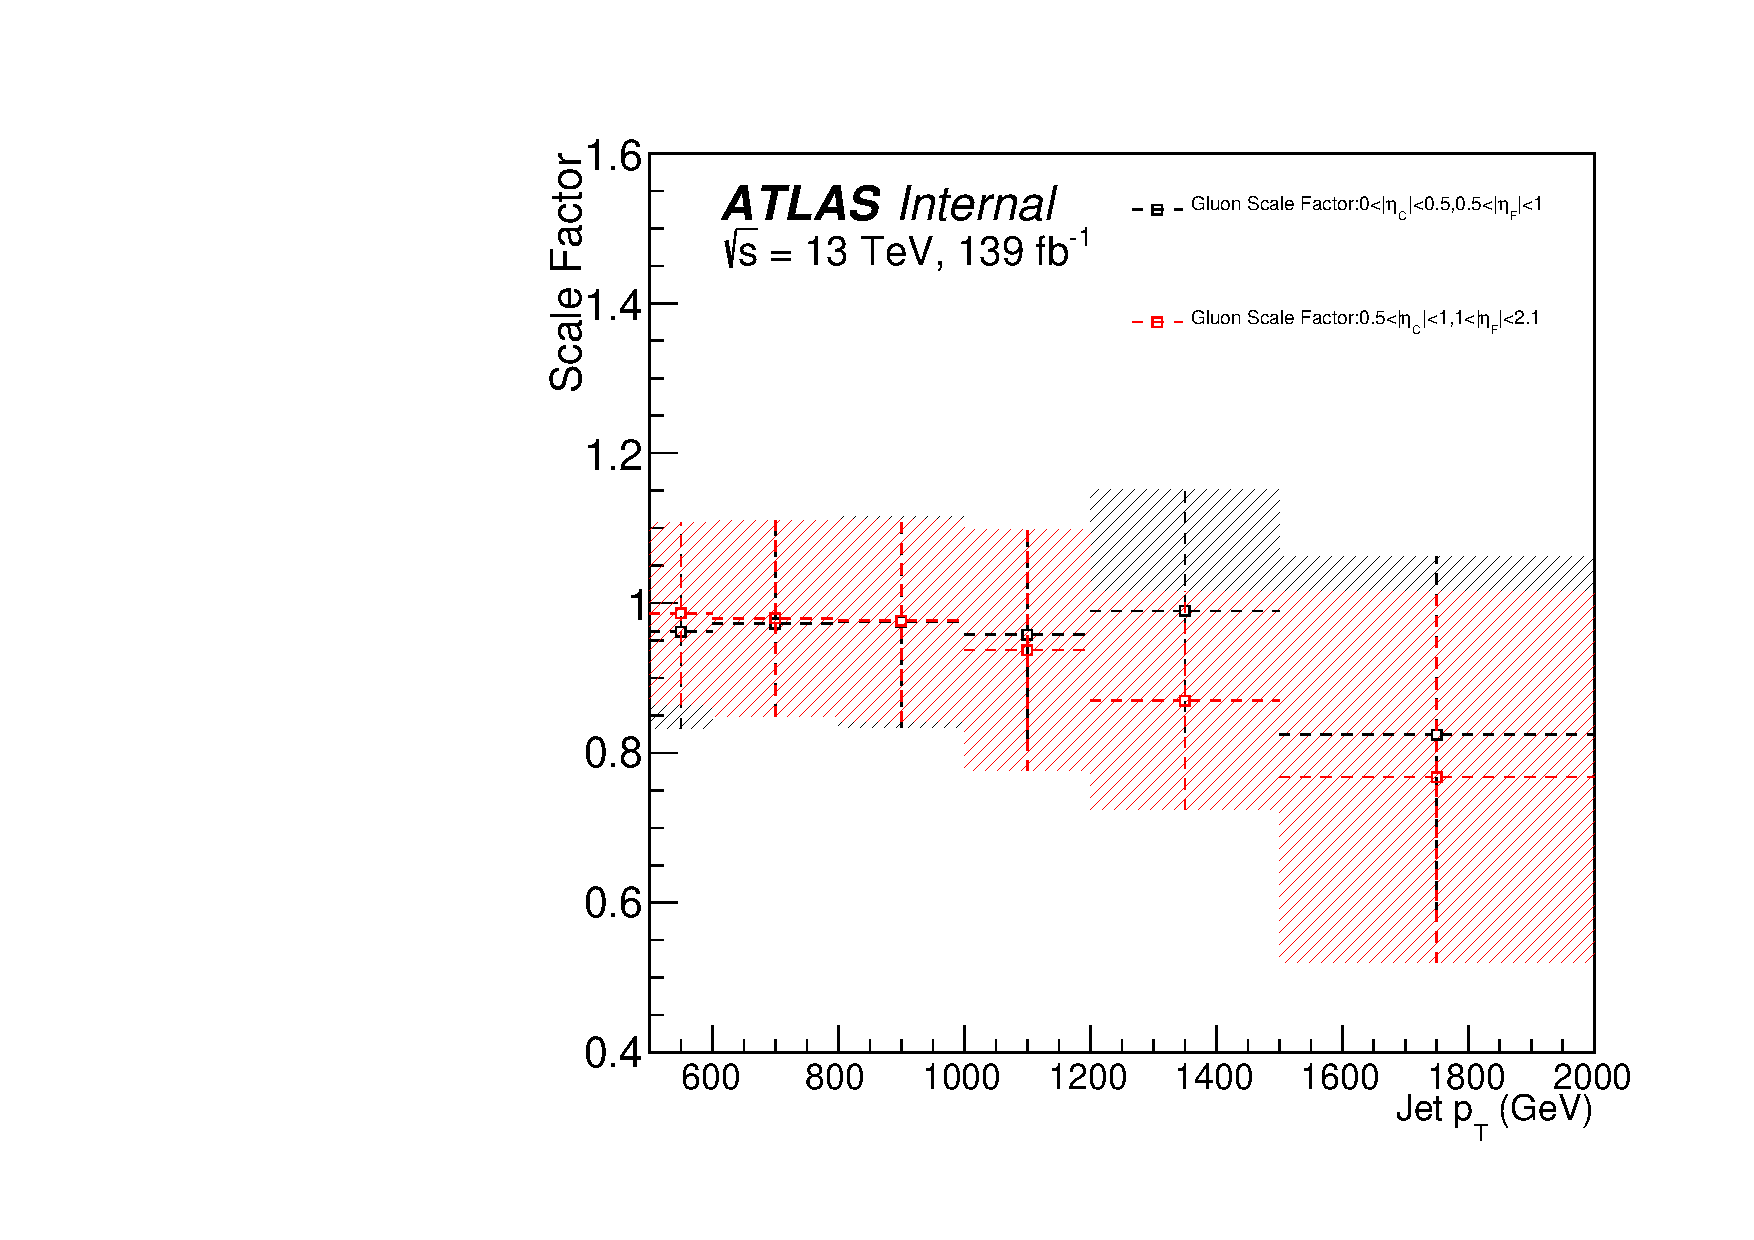
\includegraphics[width=0.45\textwidth]{fig/Method1/pythia/eta/working-point-SF-compare/0-0.5_0.5-1_0.5-1_1-2.1-Gluon-SF-0.6-ntrk.pdf}}\\
%	\caption[]{
%	For 60$\%$ working point of \ntrk ,compare quark efficiency,gluon rejection and scale factors in 0<$\mid\eta_{C}\mid$<0.5,0.5<$\mid\eta_{F}\mid$<1 and in 0.5<$\mid\eta_{C}\mid$<1,1<$\mid\eta_{F}\mid$<2.1.%
%	The left plots are for quark efficiency and quark scale factors.The right plots are for gluon rejection and gluon scale factors. %
%	\subref{fig:QG-pythia-NtrkDataQWP}  \subref{fig:QG-pythia-NtrkDataQSF} are for quark distribution and \subref{fig:QG-pythia-NtrkDataGWP}  \subref{fig:QG-pythia-NtrkDataGSF} are for gluon distribution. %
% 	The error bars include the statistical uncertainty for quark efficiency and gluon factor and include statistical and parton shower modeling uncertainty for scale factors. %
%		\label{fig:QG-pythia-eta-Ntrk-6}
%	}
%\end{figure}
%
%\begin{figure}[htb]
%	\centering
%	\subfloat[Quark,Working Point:70\%~(\pythia8)]{\label{fig:QG-pythia-NtrkDataQWP}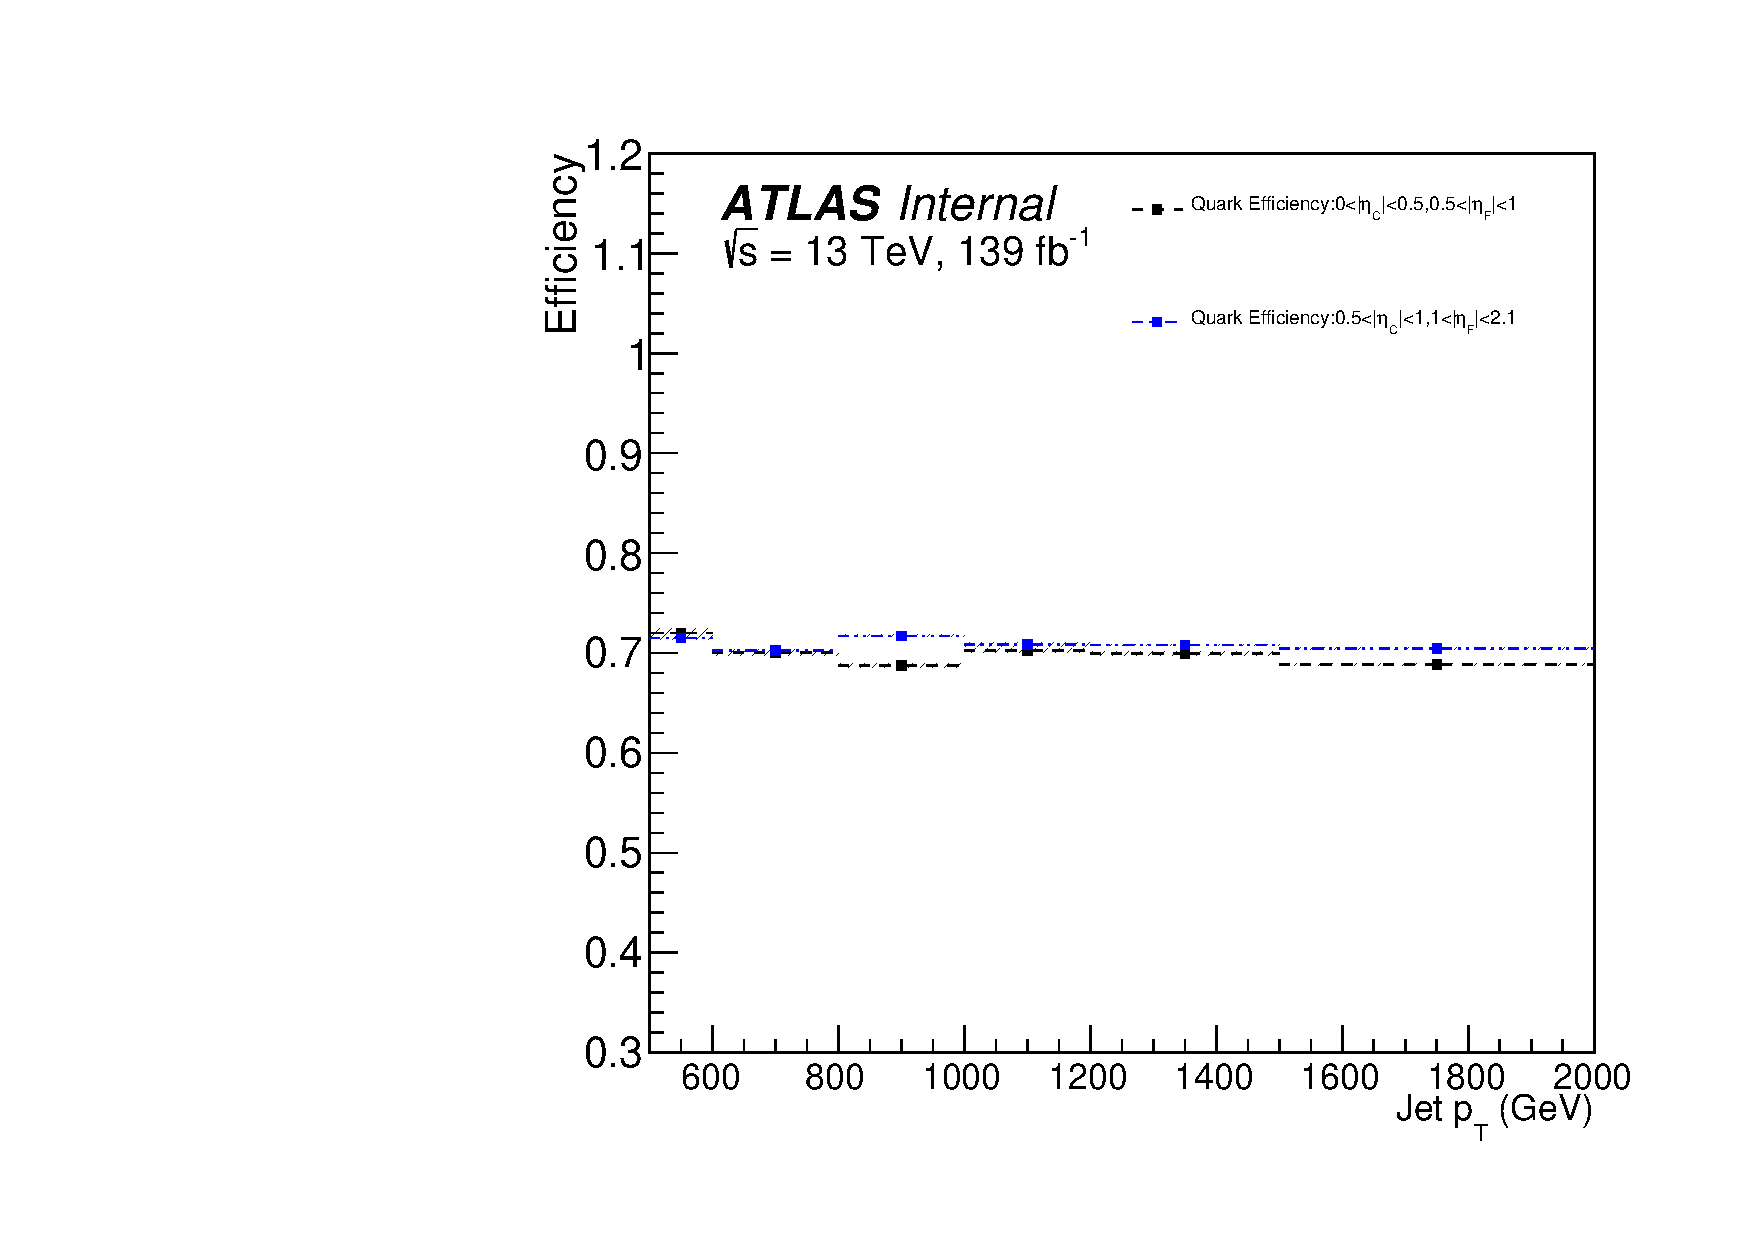
\includegraphics[width=0.45\textwidth]{fig/Method1/pythia/eta/working-point-SF-compare/0-0.5_0.5-1_0.5-1_1-2.1-Quark-WP-0.7-ntrk.pdf}} \quad
%	\subfloat[Quark,Working Point:70\%~(\pythia8)]{\label{fig:QG-pythia-NtrkDataQSF}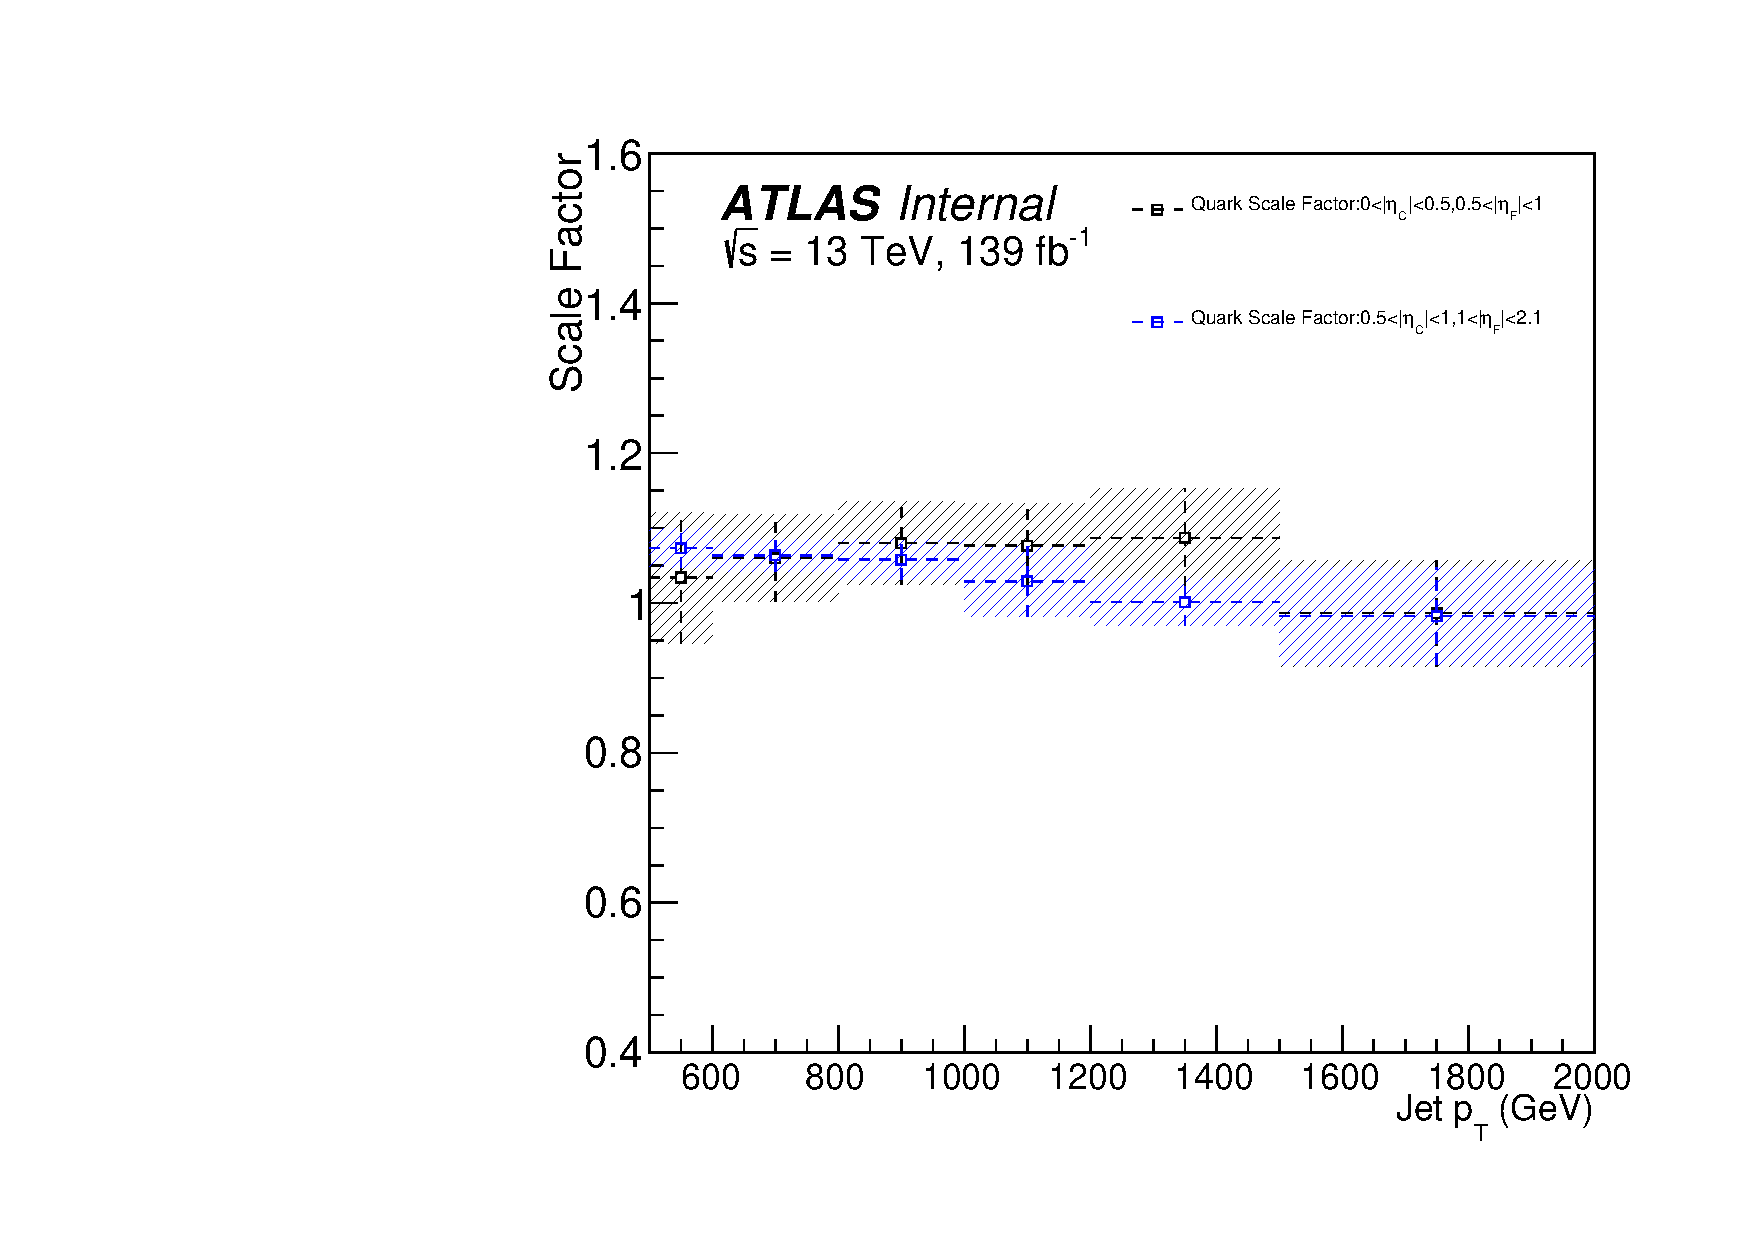
\includegraphics[width=0.45\textwidth]{fig/Method1/pythia/eta/working-point-SF-compare/0-0.5_0.5-1_0.5-1_1-2.1-Quark-SF-0.7-ntrk.pdf}}\\
%	\subfloat[Gluon,Working Point:70\%~(\pythia8)]{\label{fig:QG-pythia-NtrkDataGWP}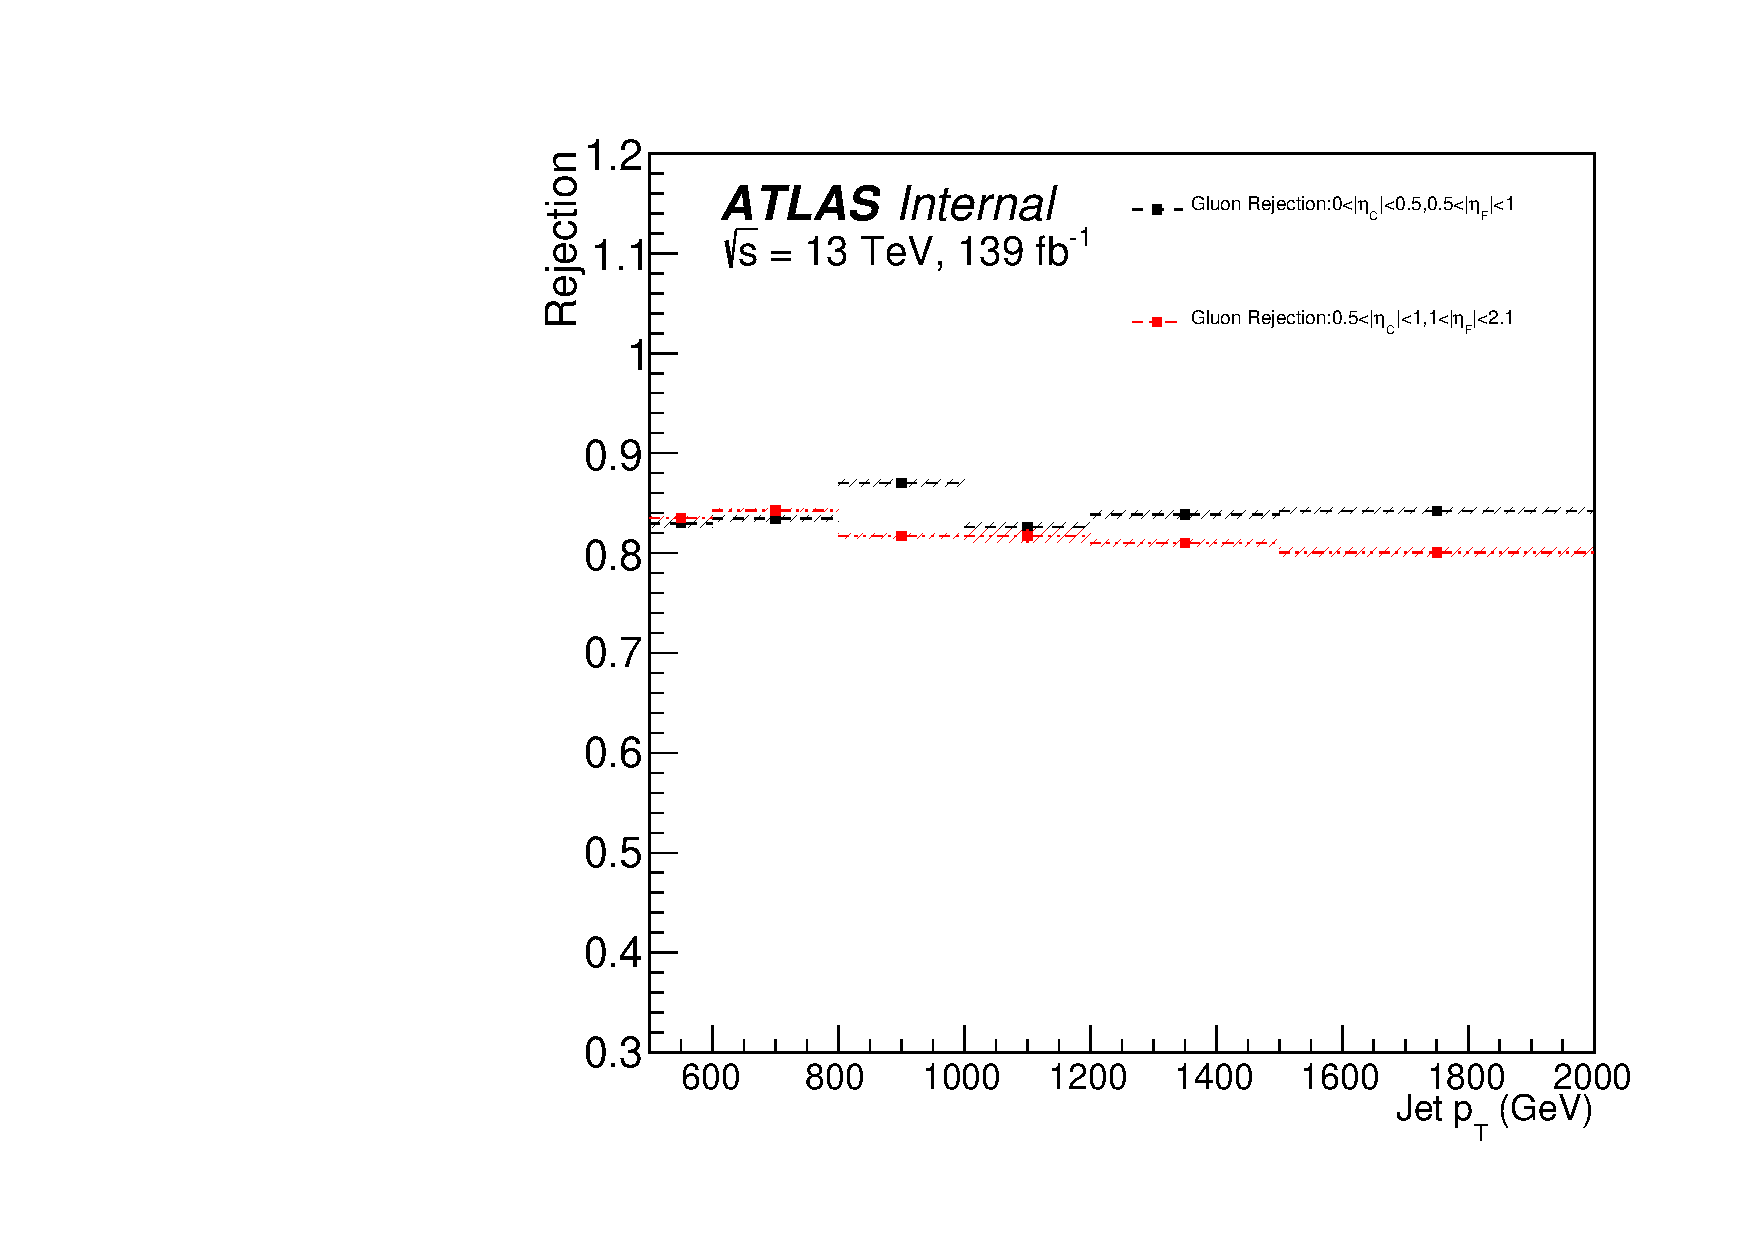
\includegraphics[width=0.45\textwidth]{fig/Method1/pythia/eta/working-point-SF-compare/0-0.5_0.5-1_0.5-1_1-2.1-Gluon-WP-0.7-ntrk.pdf}} \quad
%	\subfloat[Gluon,Working Point:70\%~(\pythia8)]{\label{fig:QG-pythia-NtrkDataGSF}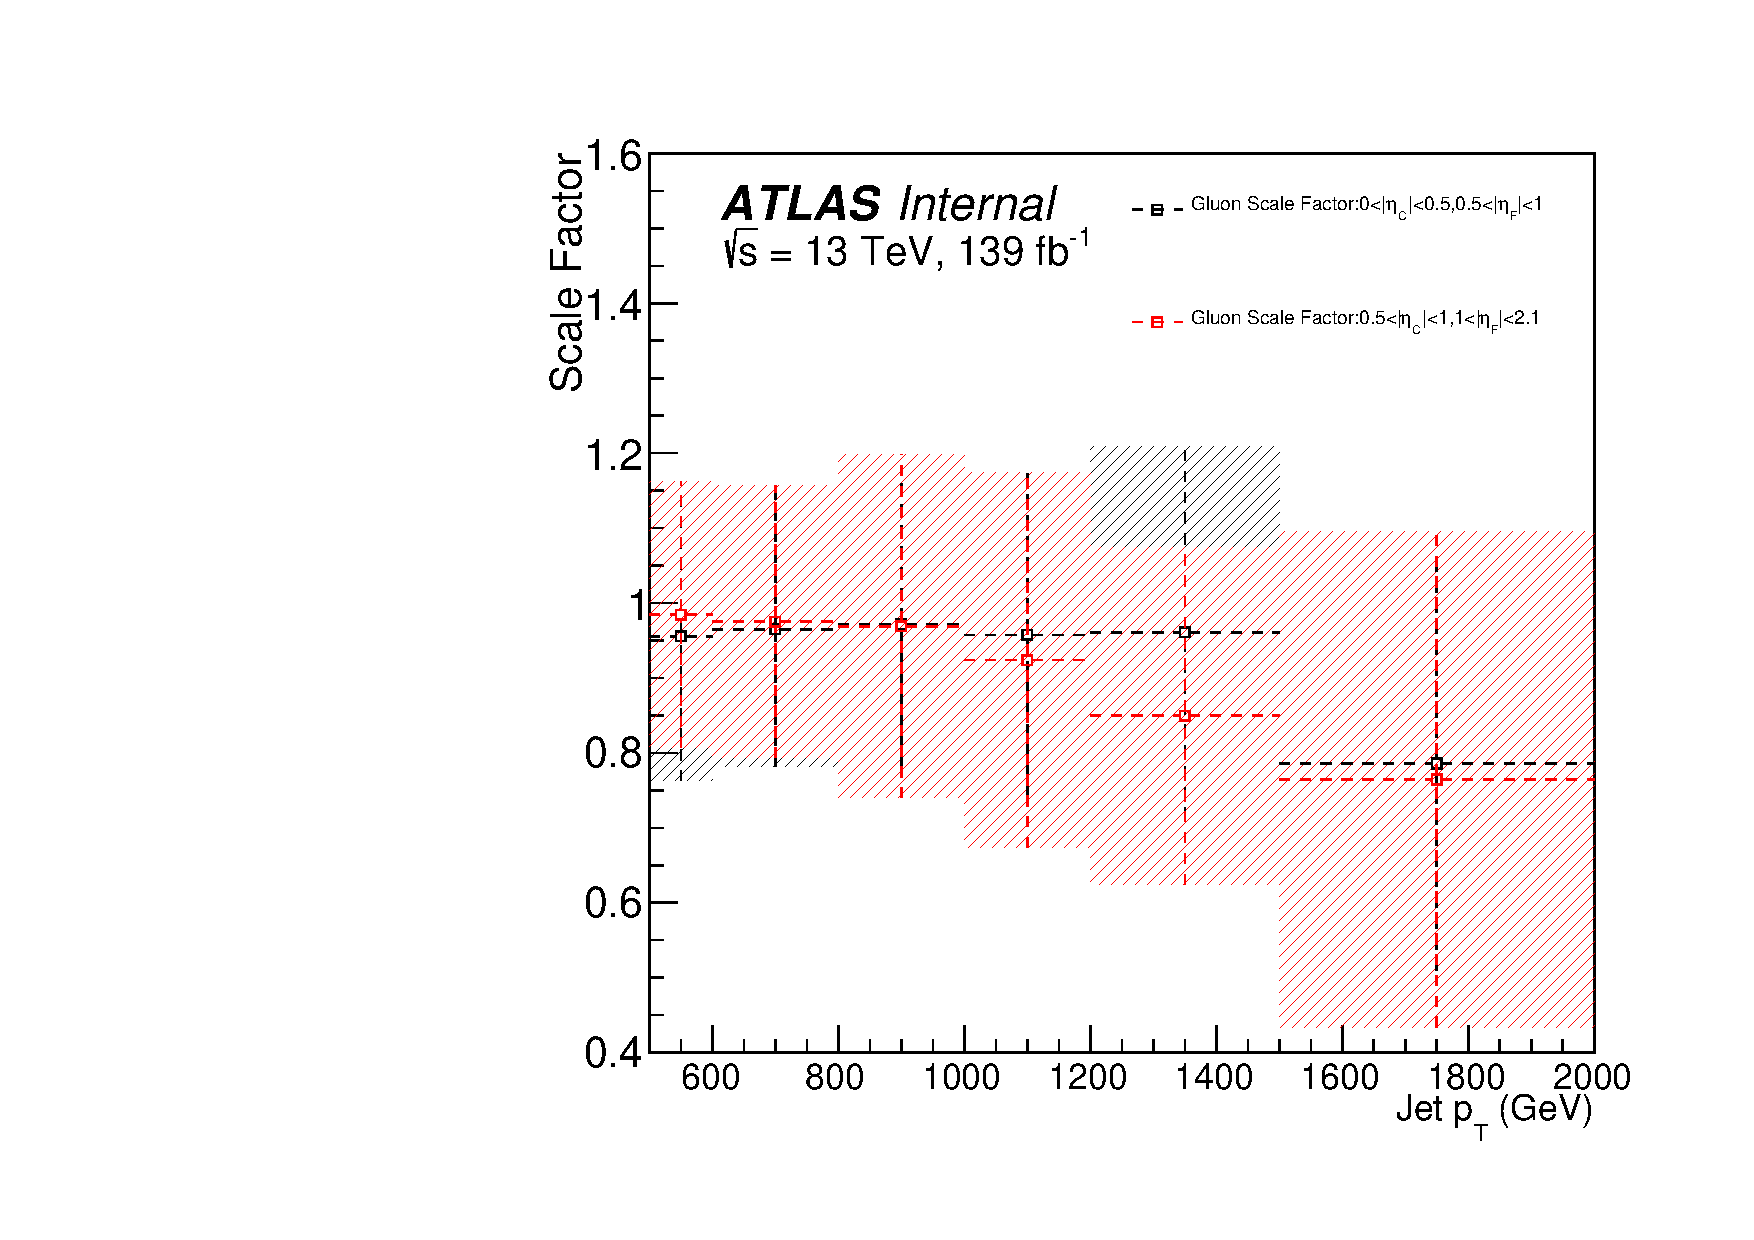
\includegraphics[width=0.45\textwidth]{fig/Method1/pythia/eta/working-point-SF-compare/0-0.5_0.5-1_0.5-1_1-2.1-Gluon-SF-0.7-ntrk.pdf}}\\
%	\caption[]{
%	For 70$\%$ working point of \ntrk ,compare quark efficiency,gluon rejection and scale factors in 0<$\mid\eta_{C}\mid$<0.5,0.5<$\mid\eta_{F}\mid$<1 and in 0.5<$\mid\eta_{C}\mid$<1,1<$\mid\eta_{F}\mid$<2.1.%
%	The left plots are for quark efficiency and quark scale factors.The right plots are for gluon rejection and gluon scale factors. %
%	\subref{fig:QG-pythia-NtrkDataQWP}  \subref{fig:QG-pythia-NtrkDataQSF} are for quark distribution and \subref{fig:QG-pythia-NtrkDataGWP}  \subref{fig:QG-pythia-NtrkDataGSF} are for gluon distribution. %
% 	The error bars include the statistical uncertainty for quark efficiency and gluon factor and include statistical and parton shower modeling uncertainty for scale factors. %
%		\label{fig:QG-pythia-eta-Ntrk-7}
%	}
%\end{figure}
%
%\begin{figure}[htb]
%	\centering
%	\subfloat[Quark,Working Point:80\%~(\pythia8)]{\label{fig:QG-pythia-NtrkDataQWP}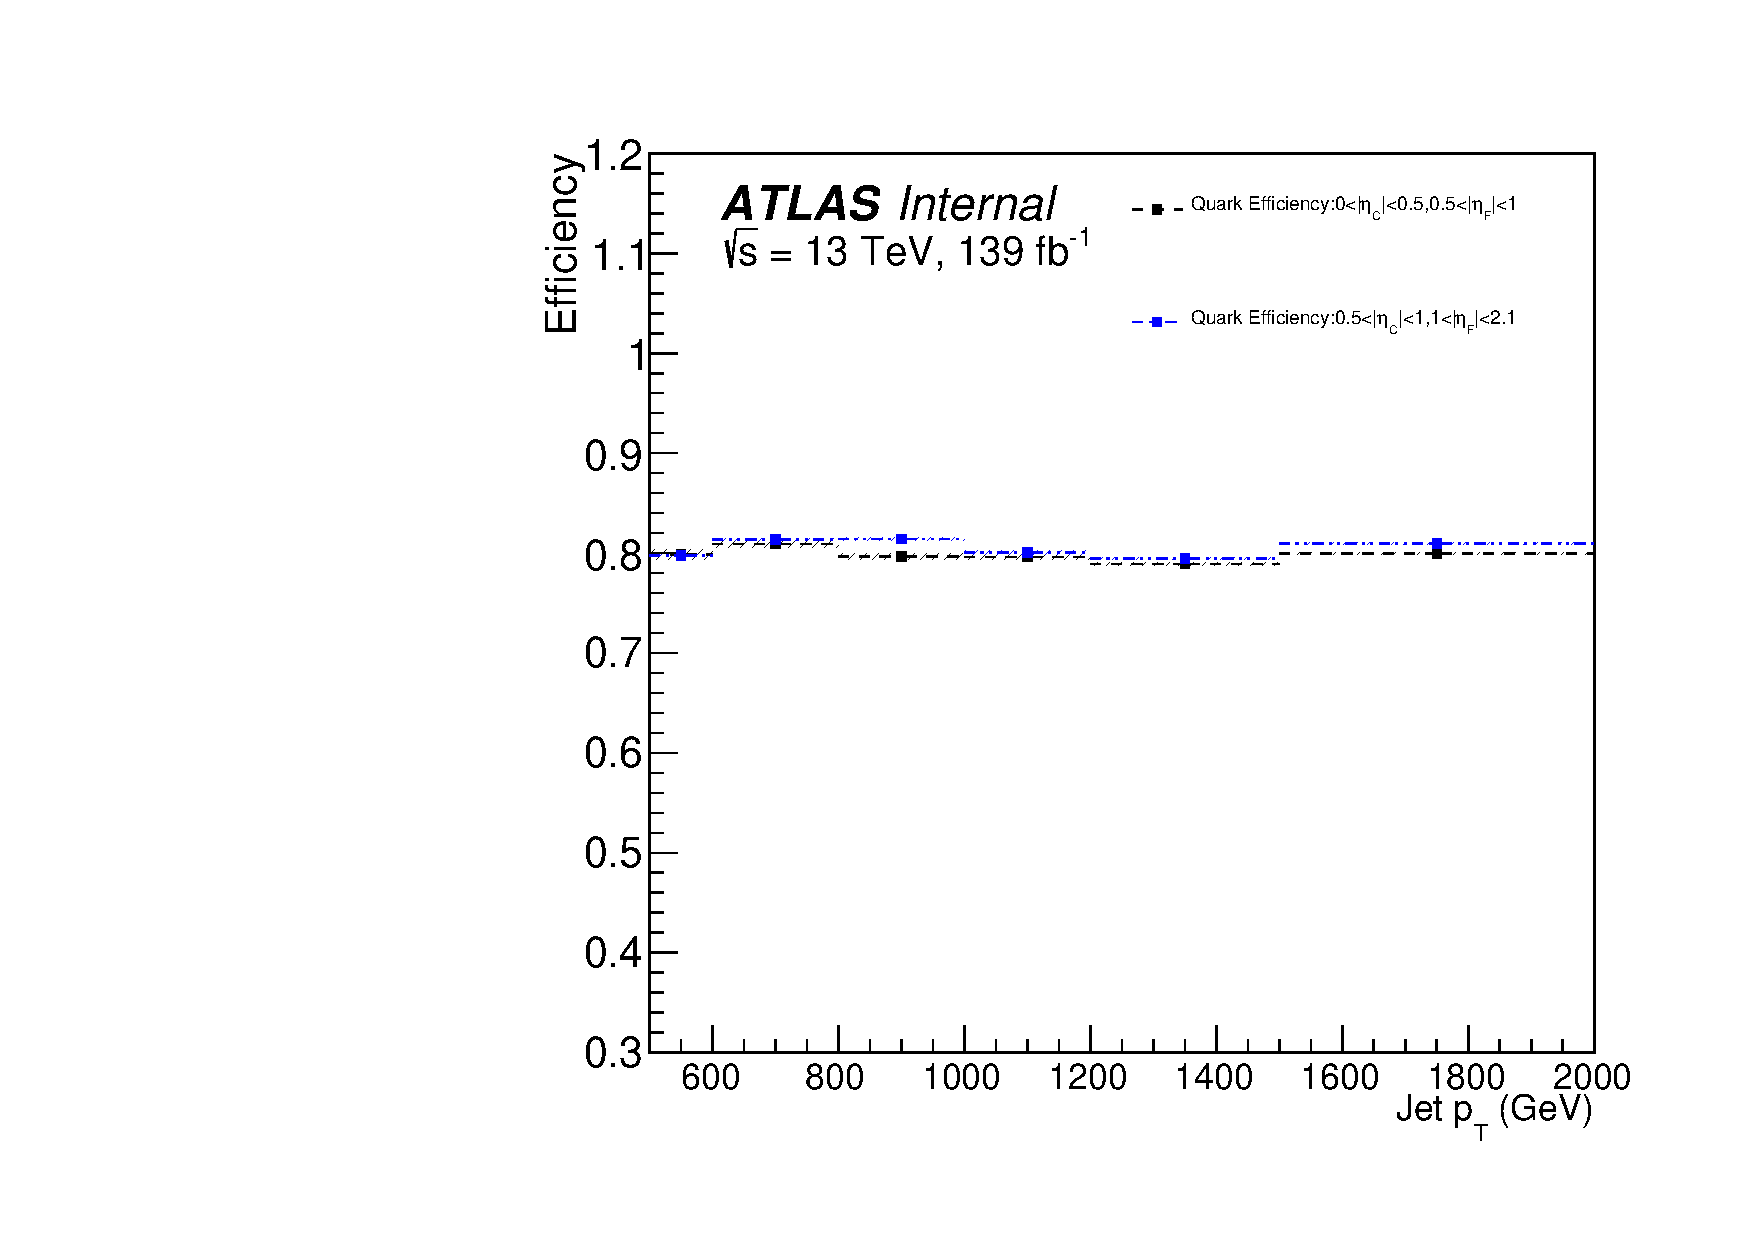
\includegraphics[width=0.45\textwidth]{fig/Method1/pythia/eta/working-point-SF-compare/0-0.5_0.5-1_0.5-1_1-2.1-Quark-WP-0.8-ntrk.pdf}} \quad
%	\subfloat[Quark,Working Point:80\%~(\pythia8)]{\label{fig:QG-pythia-NtrkDataQSF}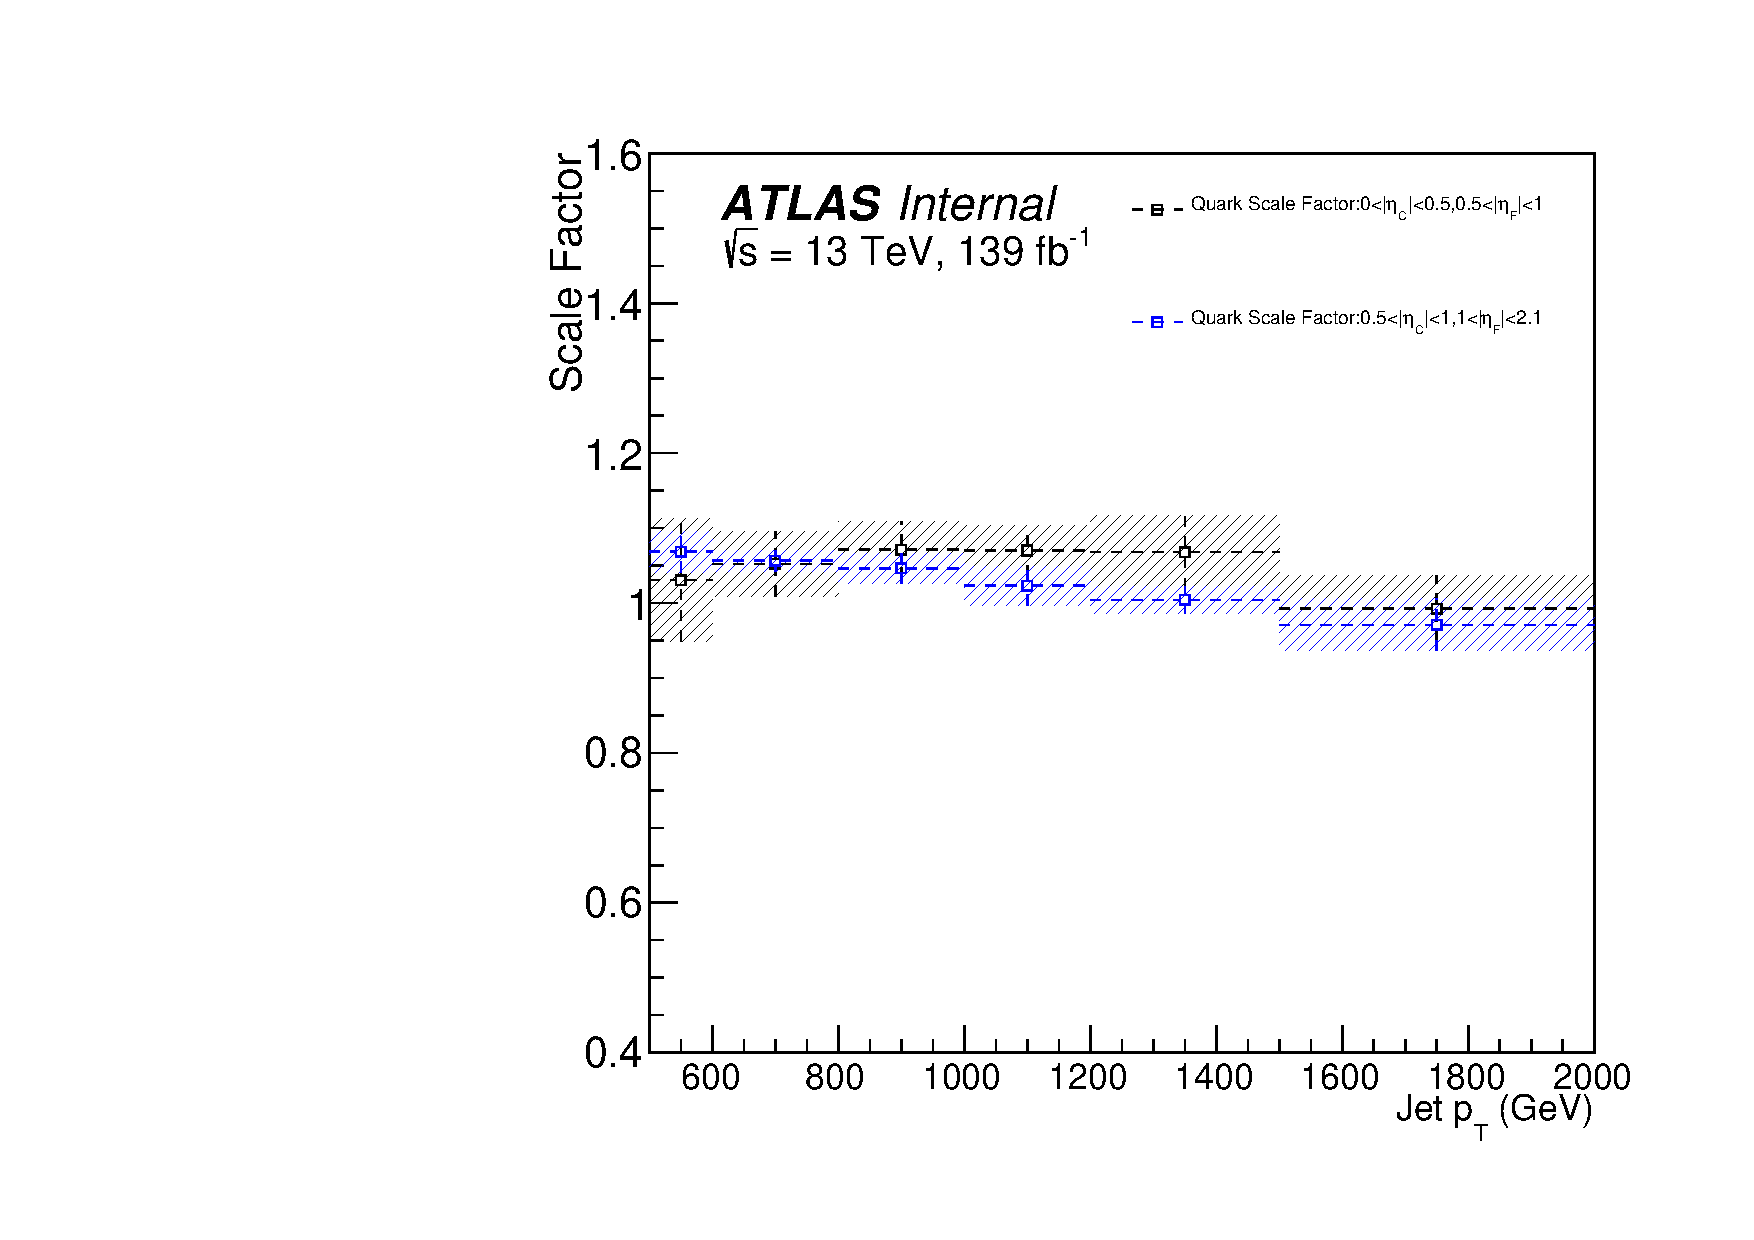
\includegraphics[width=0.45\textwidth]{fig/Method1/pythia/eta/working-point-SF-compare/0-0.5_0.5-1_0.5-1_1-2.1-Quark-SF-0.8-ntrk.pdf}}\\
%	\subfloat[Gluon,Working Point:80\%~(\pythia8)]{\label{fig:QG-pythia-NtrkDataGWP}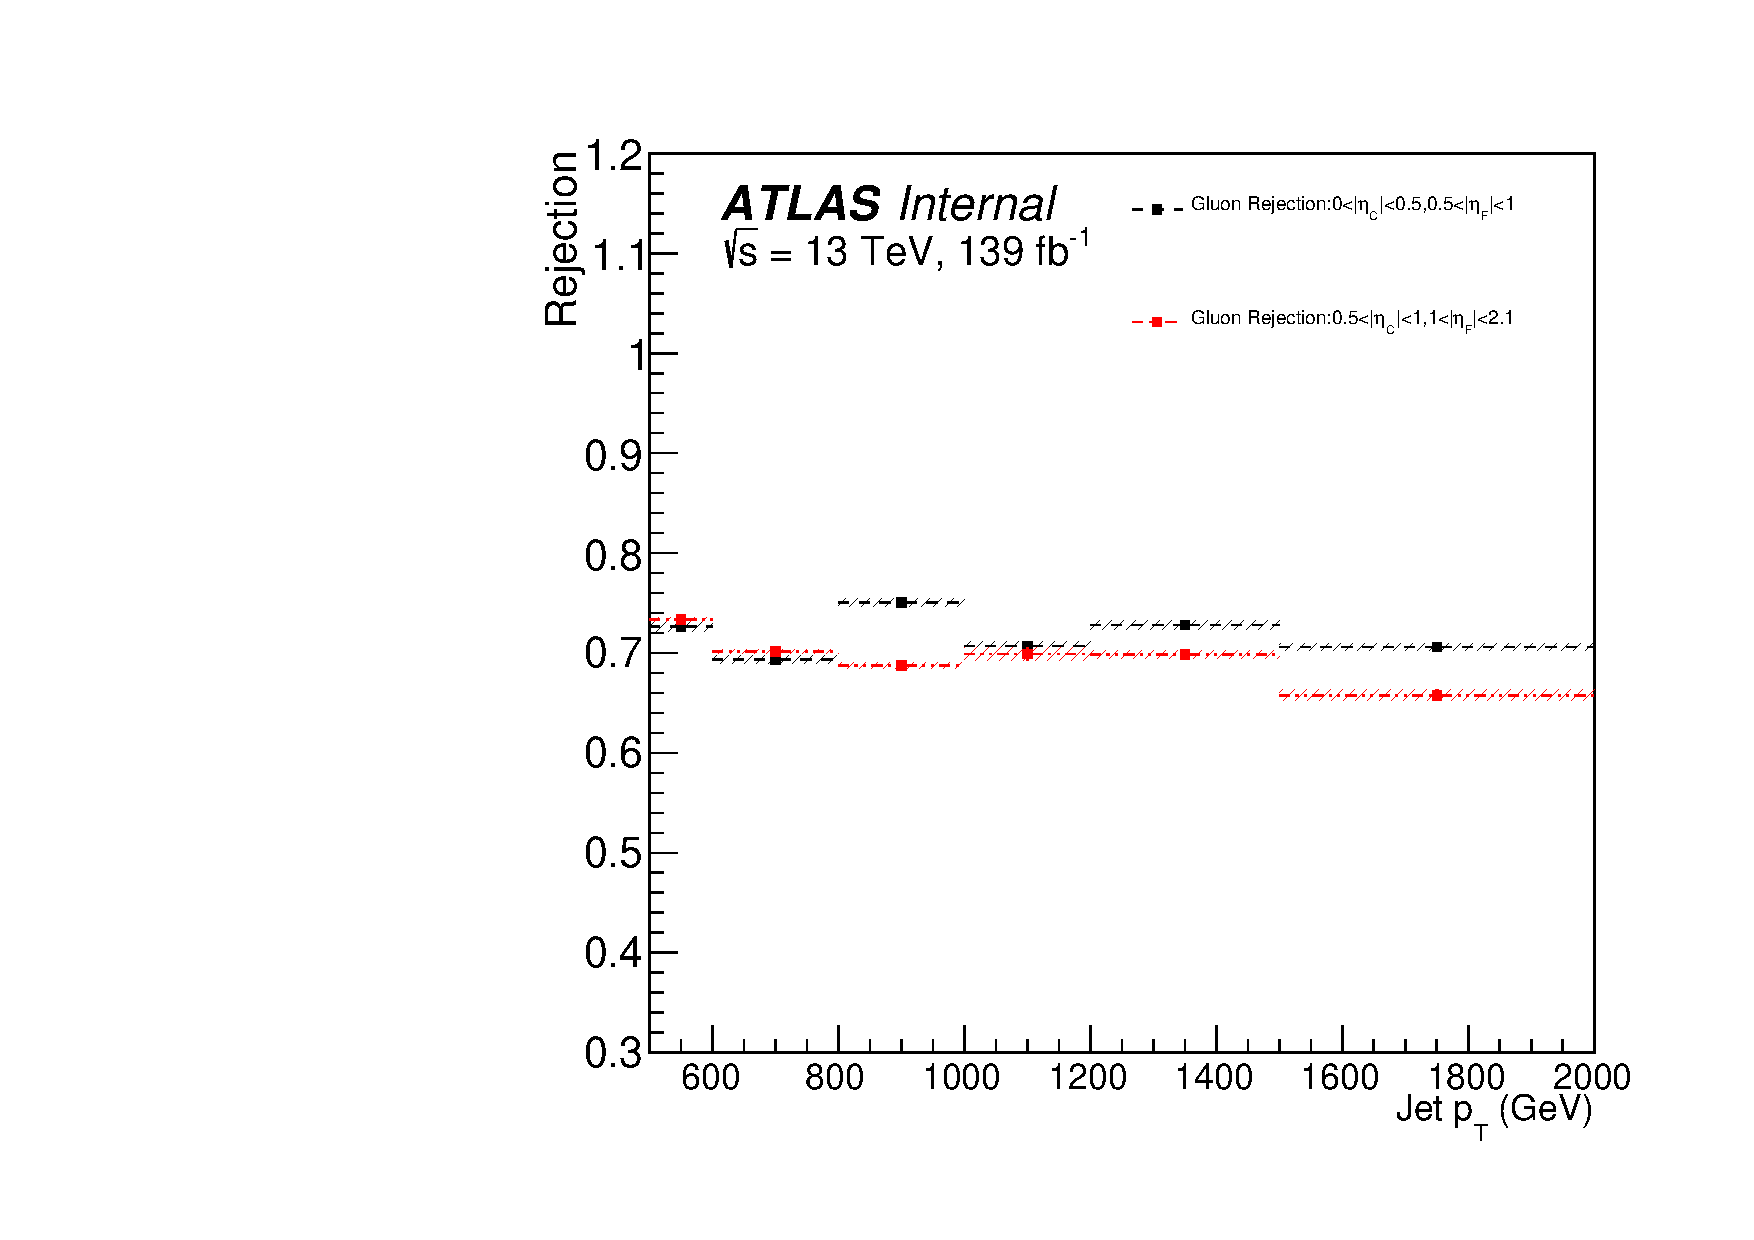
\includegraphics[width=0.45\textwidth]{fig/Method1/pythia/eta/working-point-SF-compare/0-0.5_0.5-1_0.5-1_1-2.1-Gluon-WP-0.8-ntrk.pdf}} \quad
%	\subfloat[Gluon,Working Point:80\%~(\pythia8)]{\label{fig:QG-pythia-NtrkDataGSF}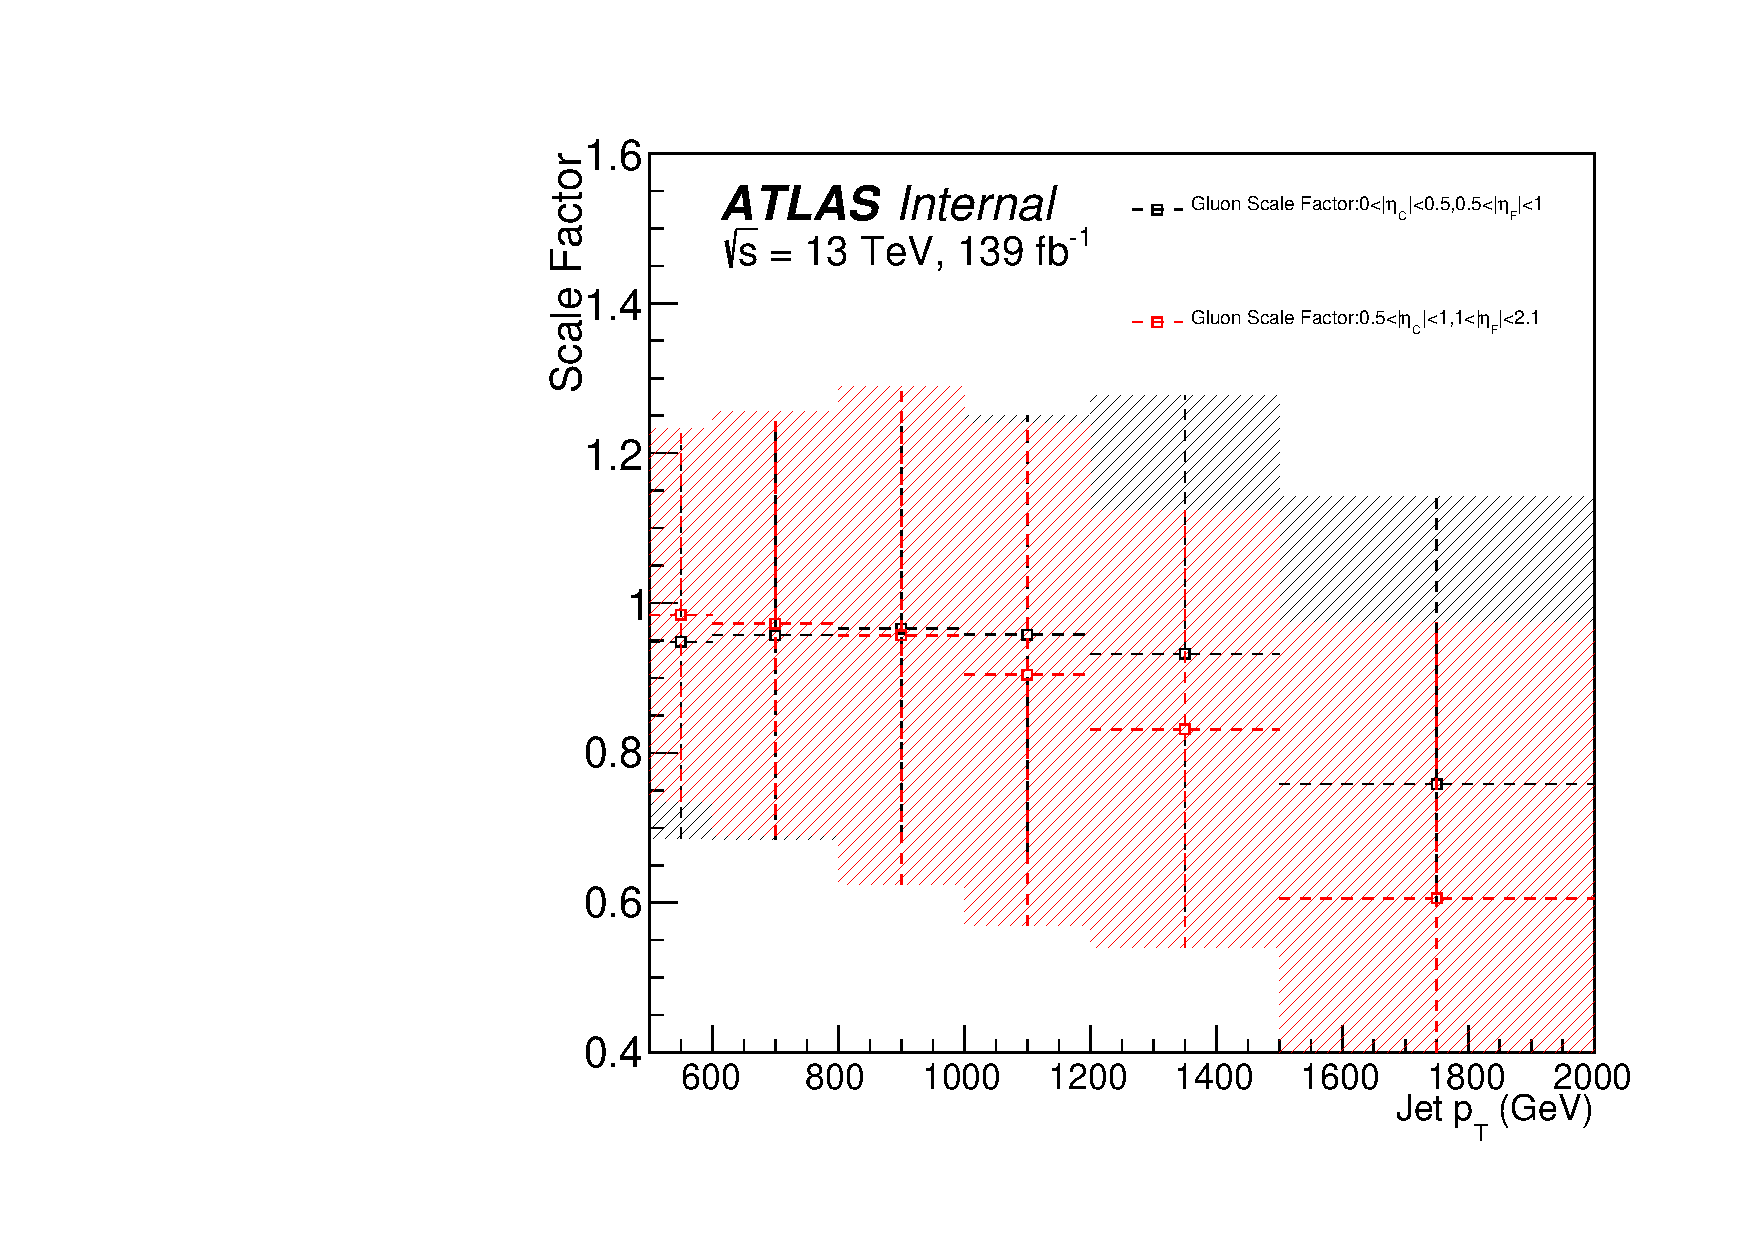
\includegraphics[width=0.45\textwidth]{fig/Method1/pythia/eta/working-point-SF-compare/0-0.5_0.5-1_0.5-1_1-2.1-Gluon-SF-0.8-ntrk.pdf}}\\
%	\caption[]{
%	For 80$\%$ working point of \ntrk ,compare quark efficiency,gluon rejection and scale factors in 0<$\mid\eta_{C}\mid$<0.5,0.5<$\mid\eta_{F}\mid$<1 and in 0.5<$\mid\eta_{C}\mid$<1,1<$\mid\eta_{F}\mid$<2.1.%
%	The left plots are for quark efficiency and quark scale factors.The right plots are for gluon rejection and gluon scale factors. %
%	\subref{fig:QG-pythia-NtrkDataQWP}  \subref{fig:QG-pythia-NtrkDataQSF} are for quark distribution and \subref{fig:QG-pythia-NtrkDataGWP}  \subref{fig:QG-pythia-NtrkDataGSF} are for gluon distribution. %
% 	The error bars include the statistical uncertainty for quark efficiency and gluon factor and include statistical and parton shower modeling uncertainty for scale factors. %
%		\label{fig:QG-pythia-eta-Ntrk-8}
%	}
%\end{figure}
%
%\begin{figure}[htb]
%	\centering
%	\subfloat[Quark,Working Point:50\%~(\pythia8)]{\label{fig:QG-pythia-BDTDataQWP}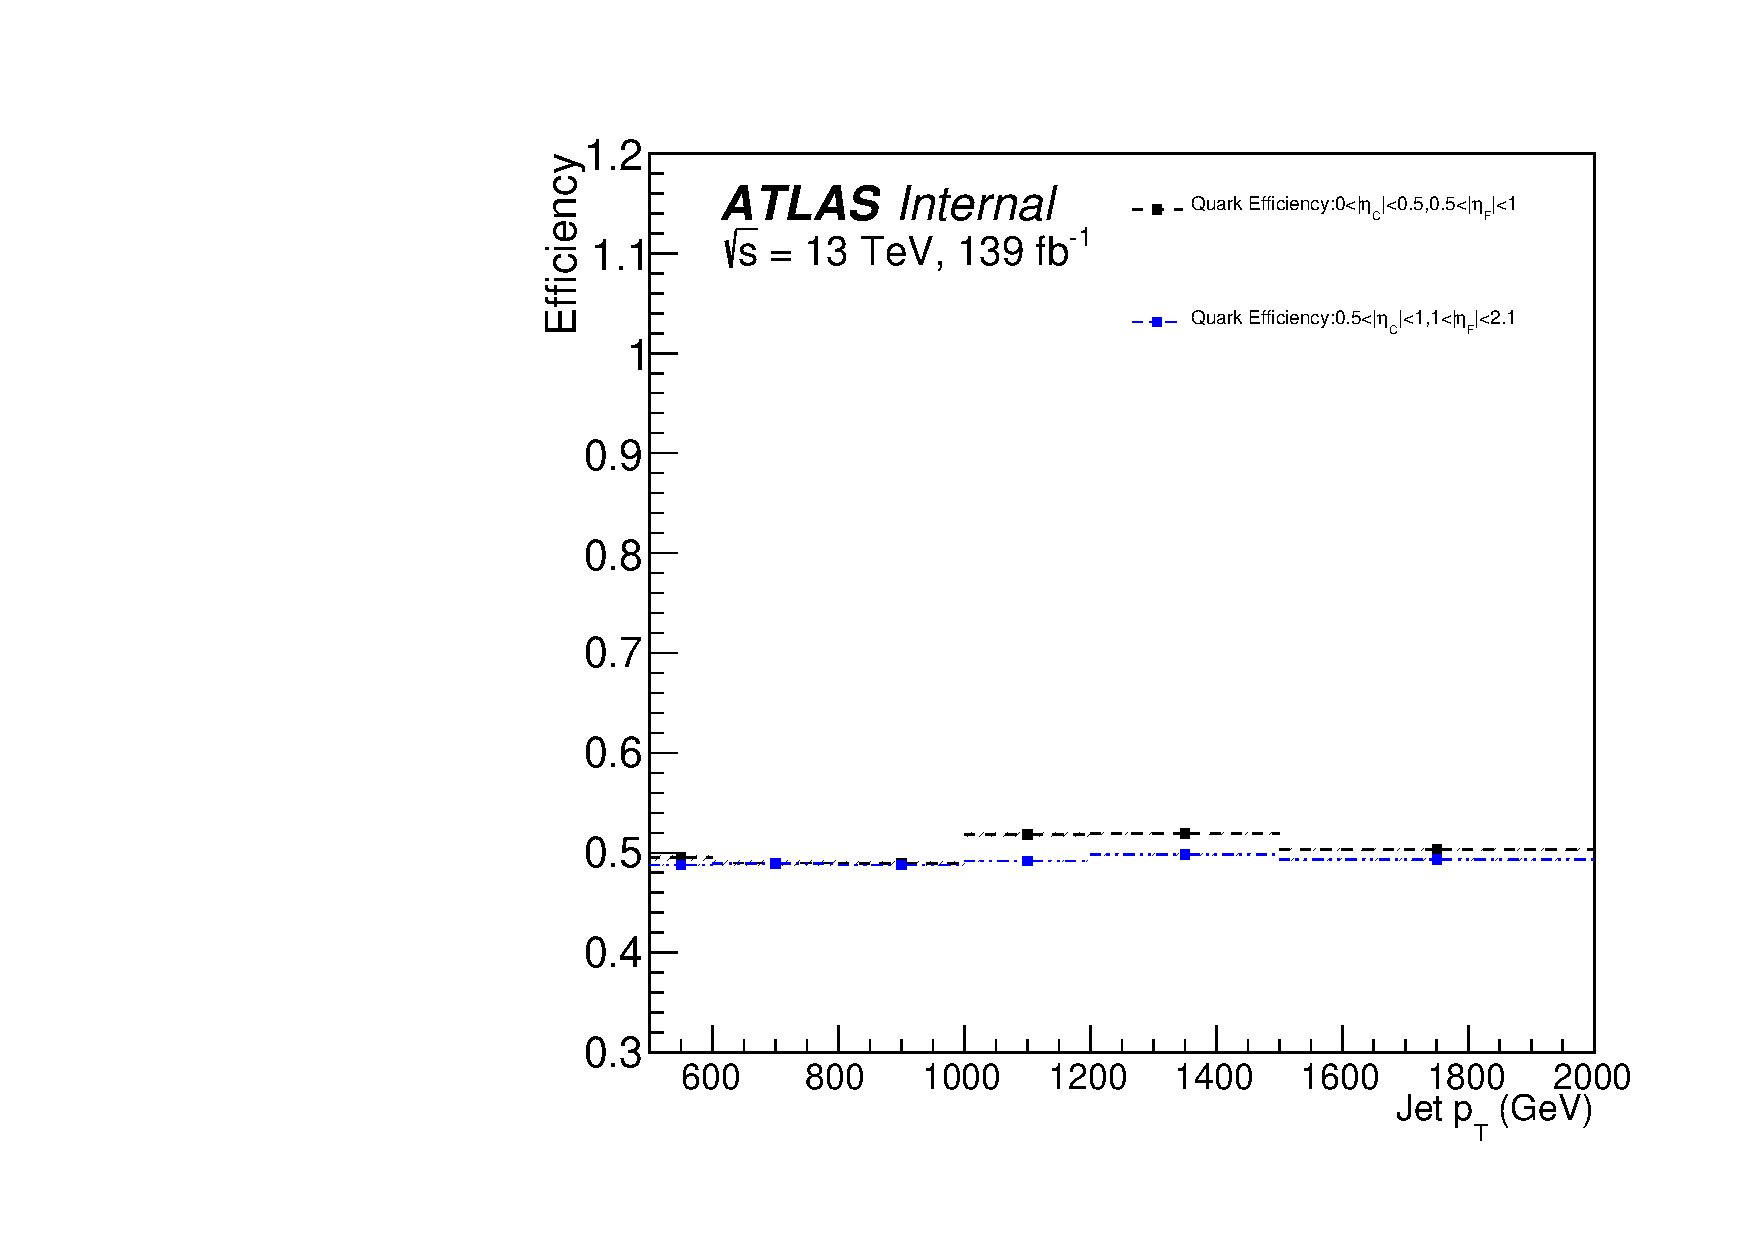
\includegraphics[width=0.45\textwidth]{fig/Method1/pythia/eta/working-point-SF-compare/0-0.5_0.5-1_0.5-1_1-2.1-Quark-WP-0.5-bdt.pdf}} \quad
%	\subfloat[Quark,Working Point:50\%~(\pythia8)]{\label{fig:QG-pythia-BDTDataQSF}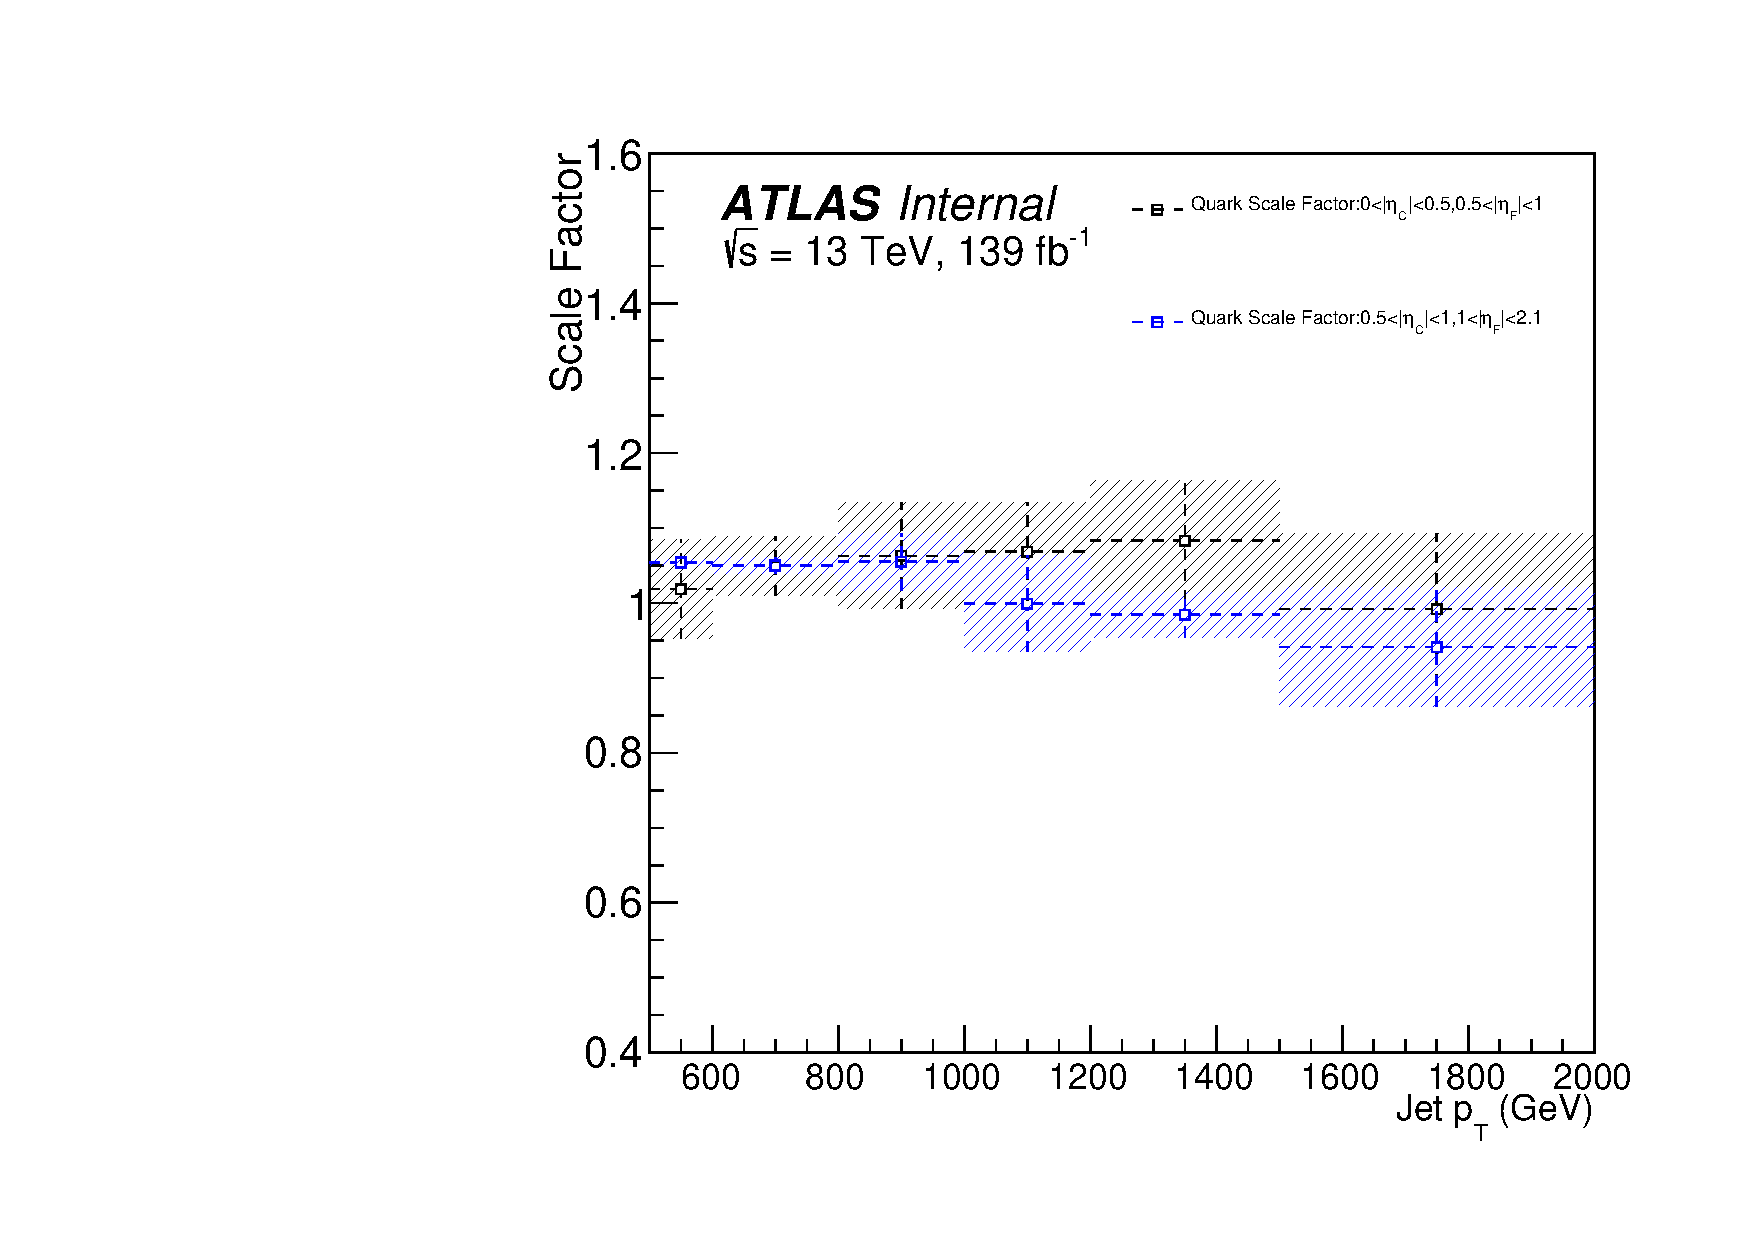
\includegraphics[width=0.45\textwidth]{fig/Method1/pythia/eta/working-point-SF-compare/0-0.5_0.5-1_0.5-1_1-2.1-Quark-SF-0.5-bdt.pdf}}\\
%	\subfloat[Gluon,Working Point:50\%~(\pythia8)]{\label{fig:QG-pythia-BDTDataGWP}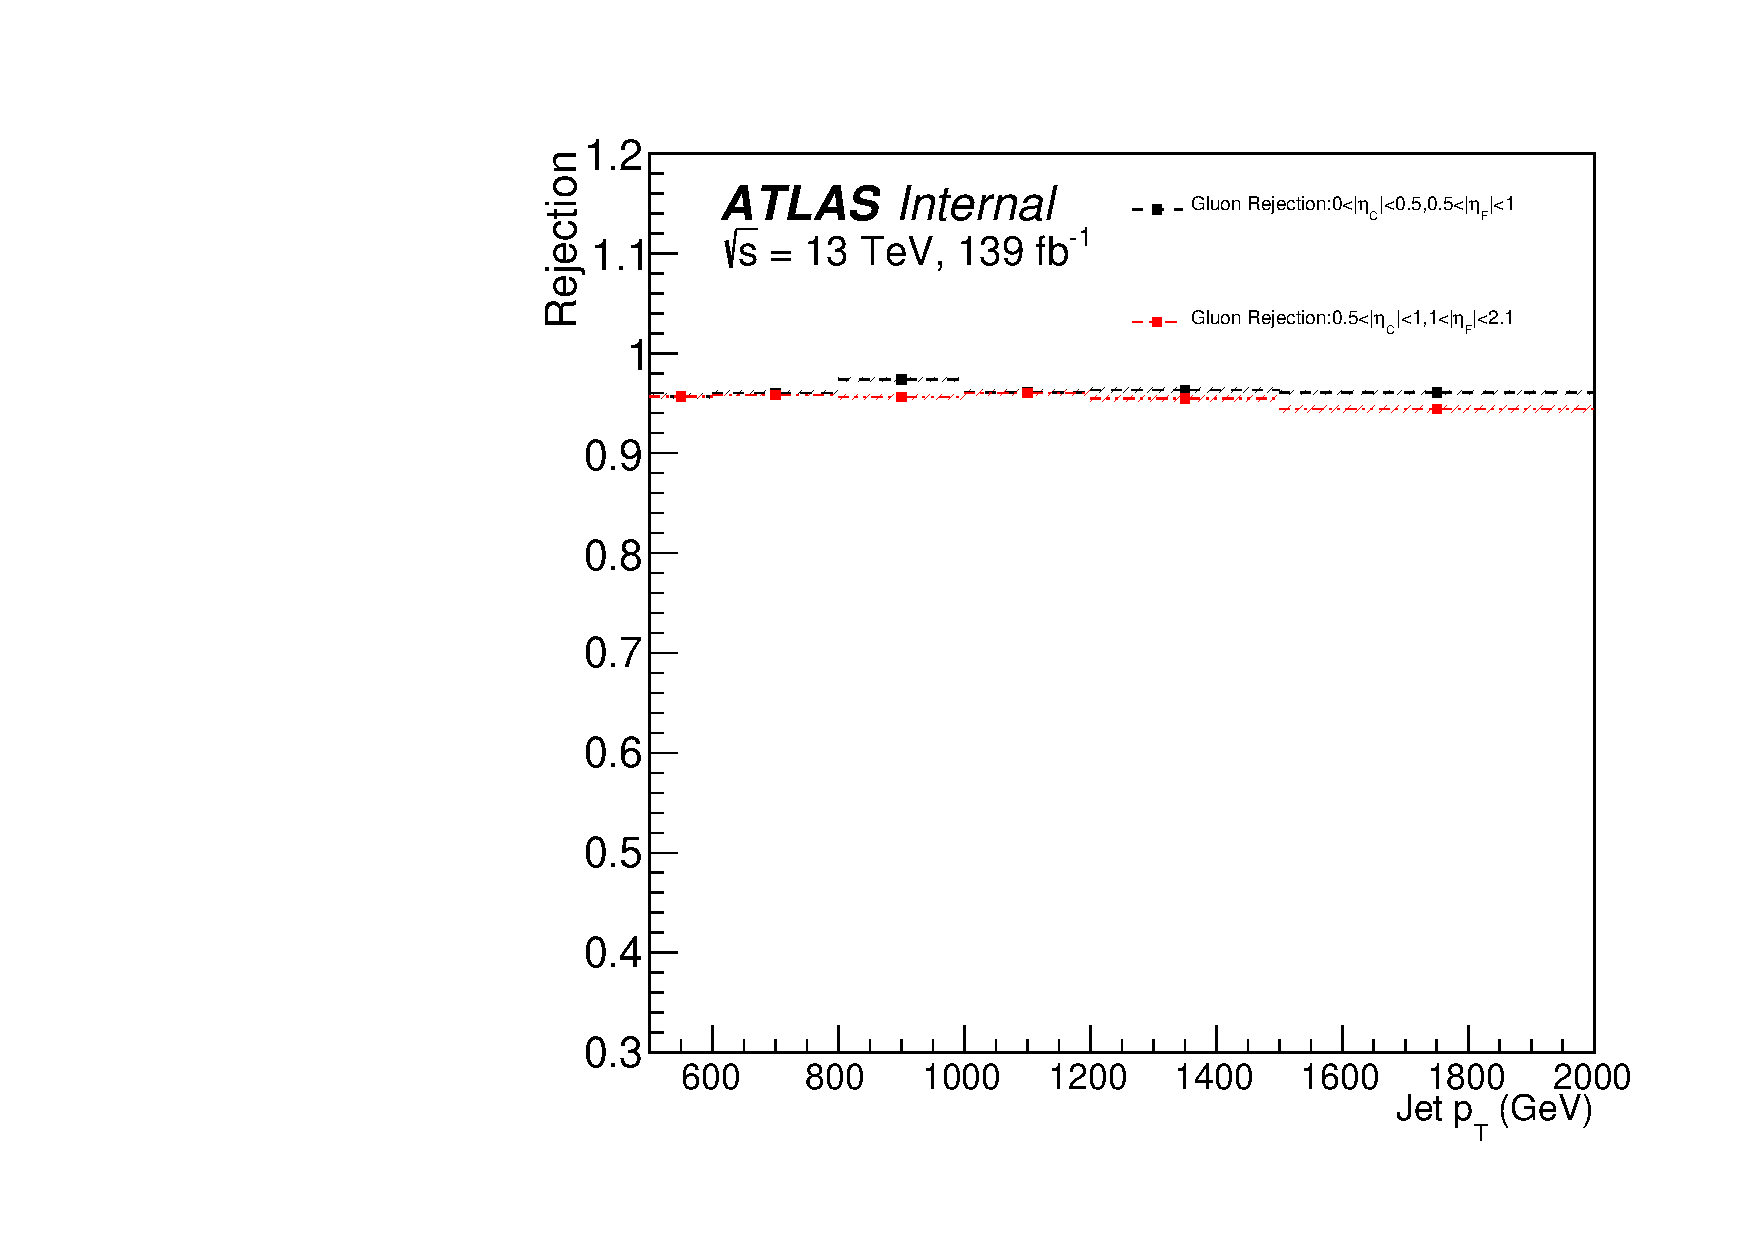
\includegraphics[width=0.45\textwidth]{fig/Method1/pythia/eta/working-point-SF-compare/0-0.5_0.5-1_0.5-1_1-2.1-Gluon-WP-0.5-bdt.pdf}} \quad
%	\subfloat[Gluon,Working Point:50\%~(\pythia8)]{\label{fig:QG-pythia-BDTDataGSF}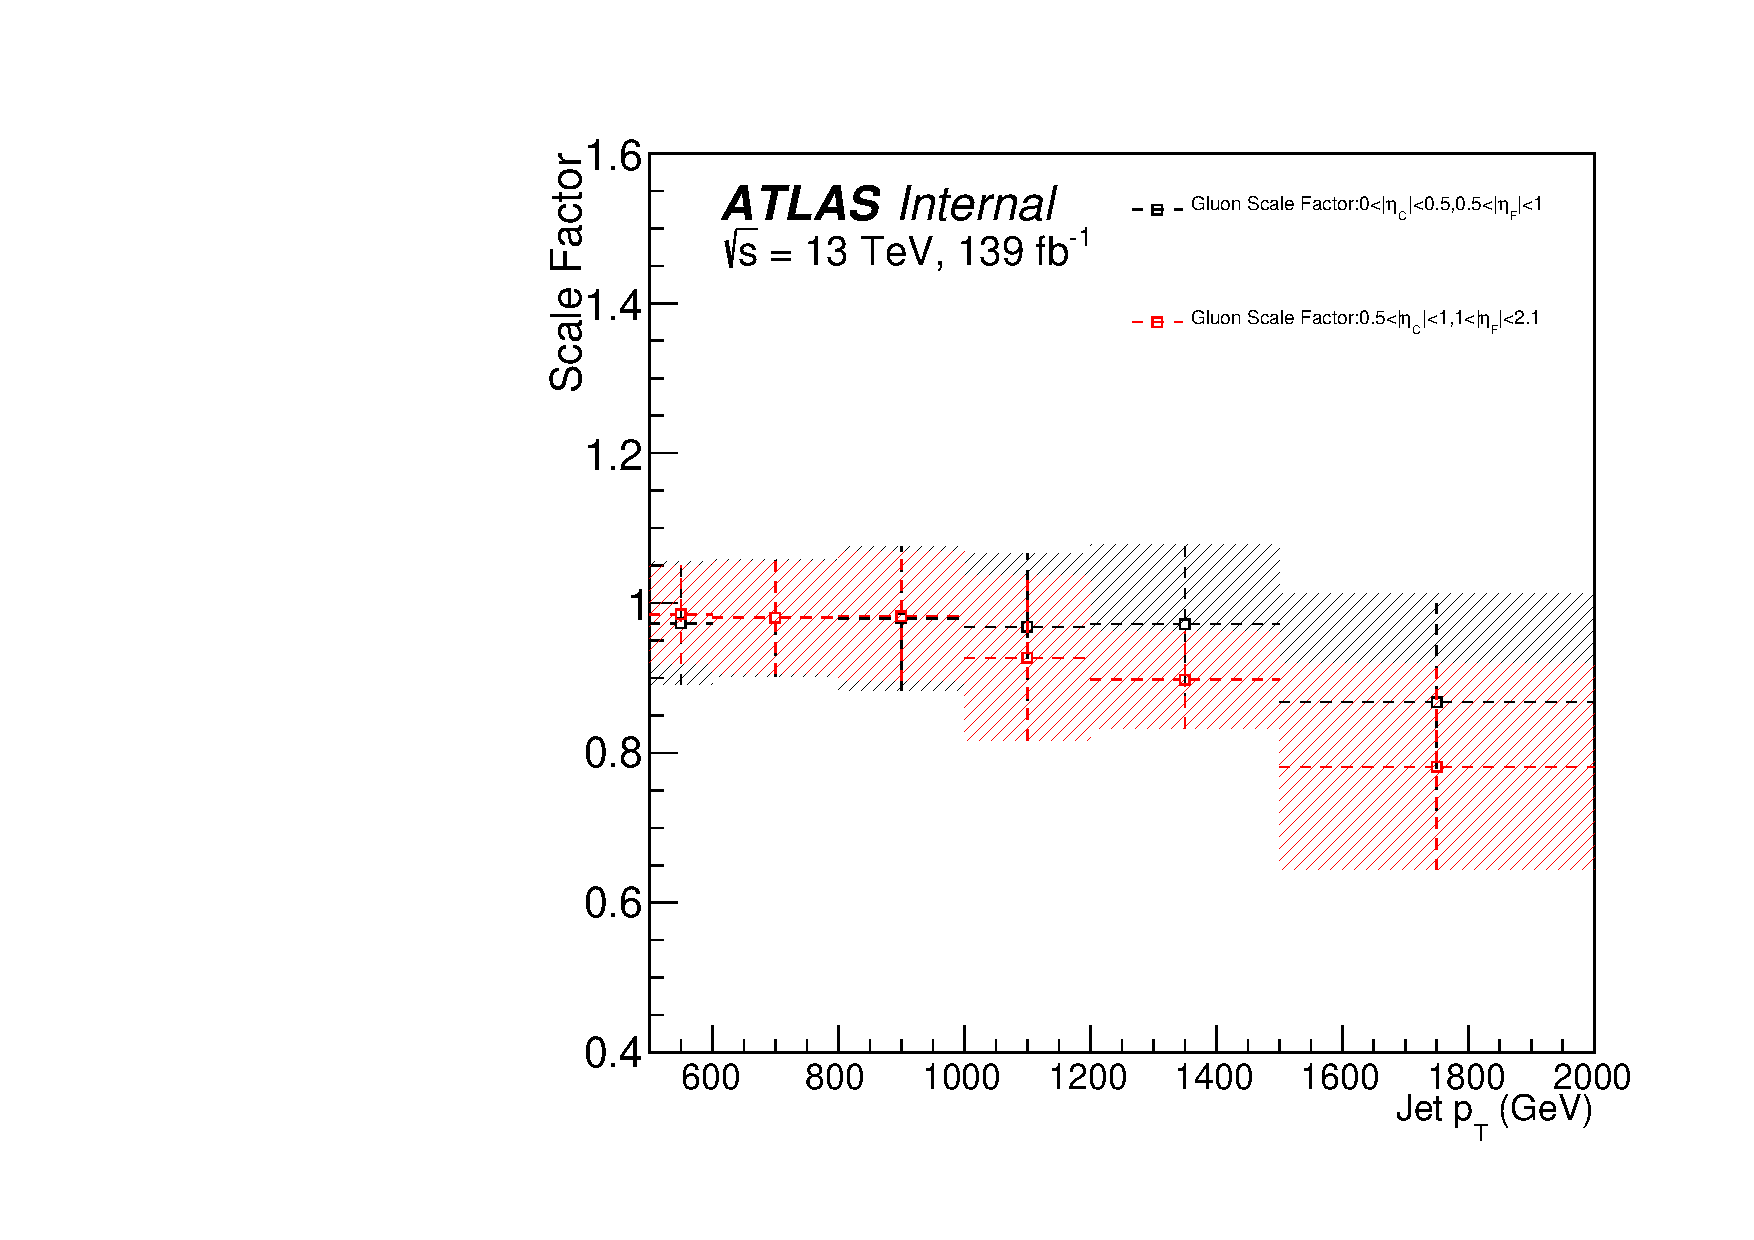
\includegraphics[width=0.45\textwidth]{fig/Method1/pythia/eta/working-point-SF-compare/0-0.5_0.5-1_0.5-1_1-2.1-Gluon-SF-0.5-bdt.pdf}}\\
%	\caption[]{
%	For 50$\%$ working point of BDT ,compare quark efficiency,gluon rejection and scale factors in 0<$\mid\eta_{C}\mid$<0.5,0.5<$\mid\eta_{F}\mid$<1 and in 0.5<$\mid\eta_{C}\mid$<1,1<$\mid\eta_{F}\mid$<2.1.%
%	The left plots are for quark efficiency and gluon rejection and the right plots are for scale factors. %
%	\subref{fig:QG-pythia-BDTDataQWP}  \subref{fig:QG-pythia-BDTDataQSF} are for quark distribution and \subref{fig:QG-pythia-BDTDataGWP}  \subref{fig:QG-pythia-BDTDataGSF} are for gluon distribution. %
% 	The error bars include the statistical uncertainty for quark efficiency and gluon factor and include statistical and parton shower modeling uncertainty for scale factors. %
%		\label{fig:QG-pythia-eta-BDT-5}
%	}
%\end{figure}
%
%\begin{figure}[htb]
%	\centering
%	\subfloat[Quark,Working Point:60\%~(\pythia8)]{\label{fig:QG-pythia-BDTDataQWP}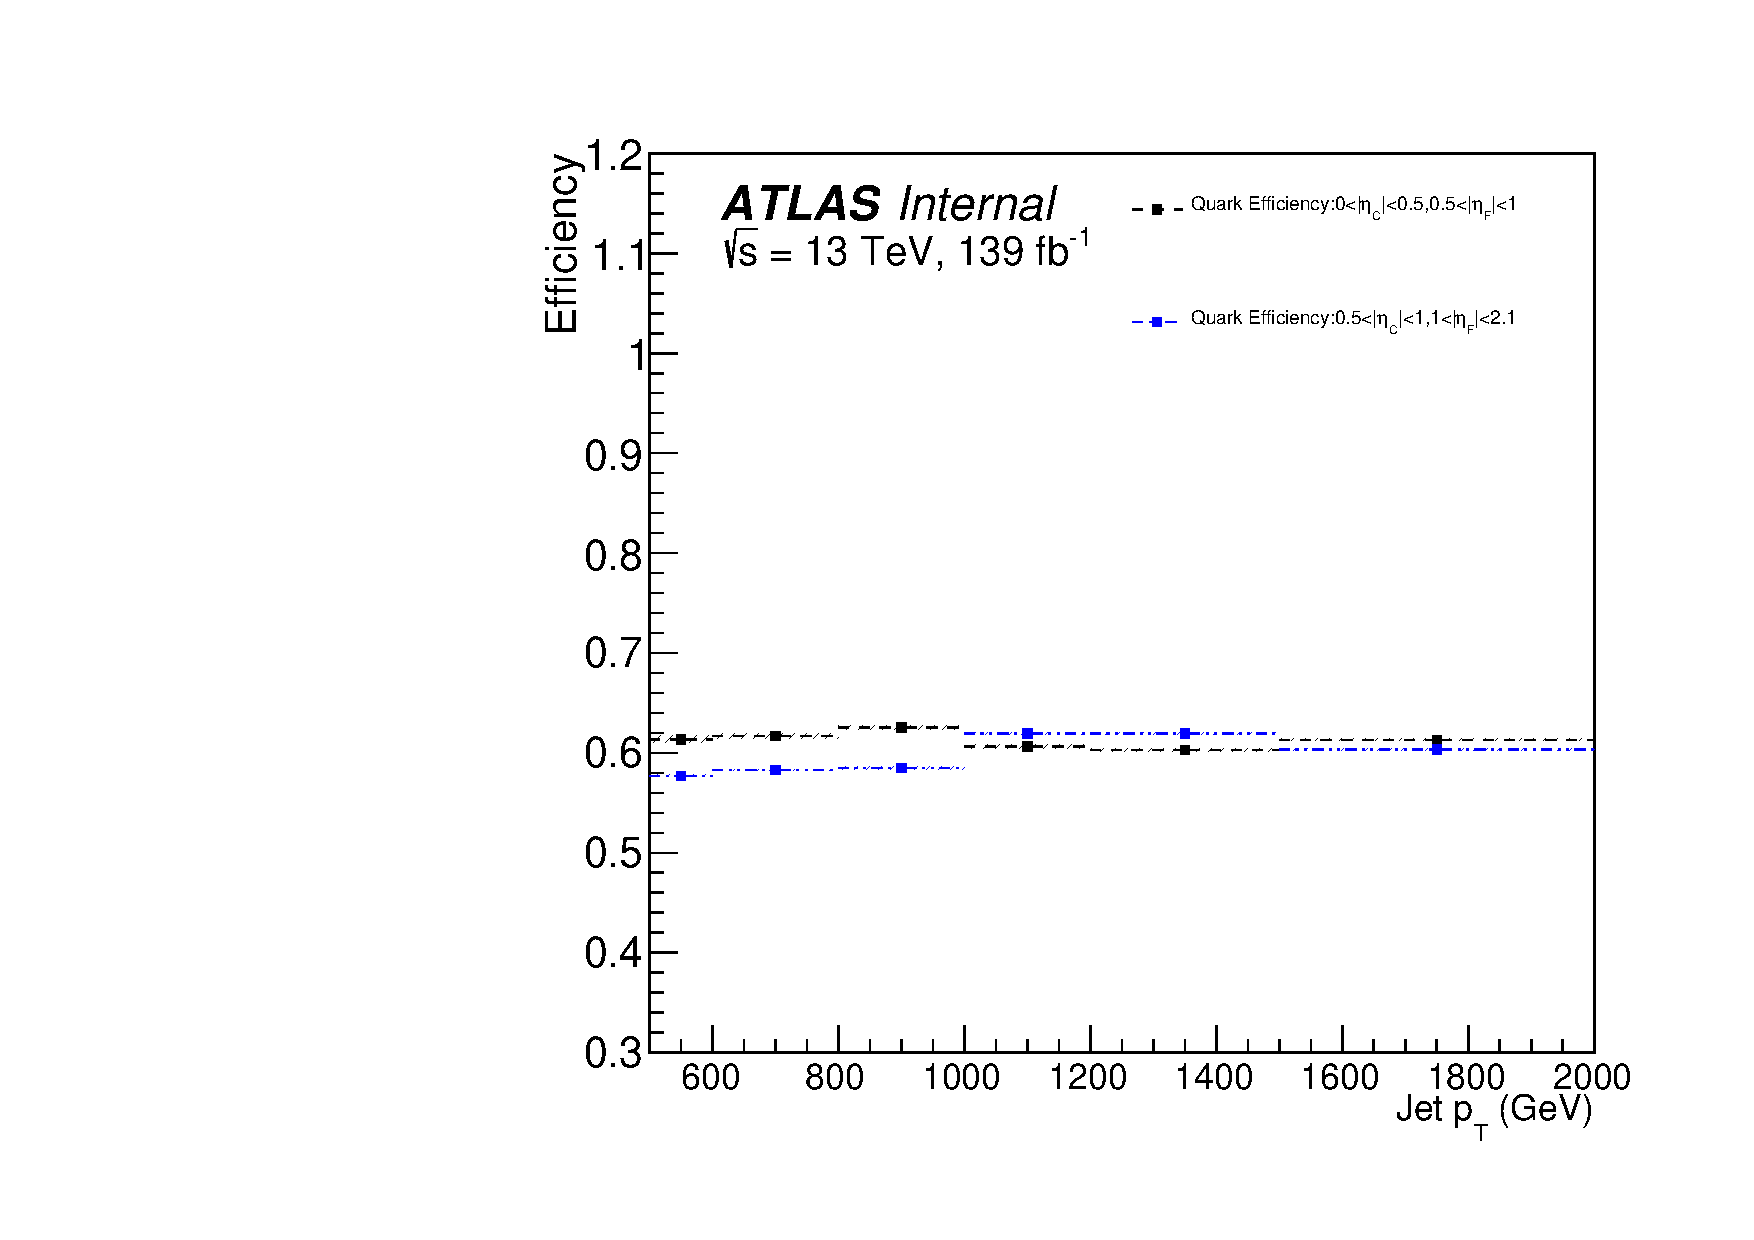
\includegraphics[width=0.45\textwidth]{fig/Method1/pythia/eta/working-point-SF-compare/0-0.5_0.5-1_0.5-1_1-2.1-Quark-WP-0.6-bdt.pdf}} \quad
%	\subfloat[Quark,Working Point:60\%~(\pythia8)]{\label{fig:QG-pythia-BDTDataQSF}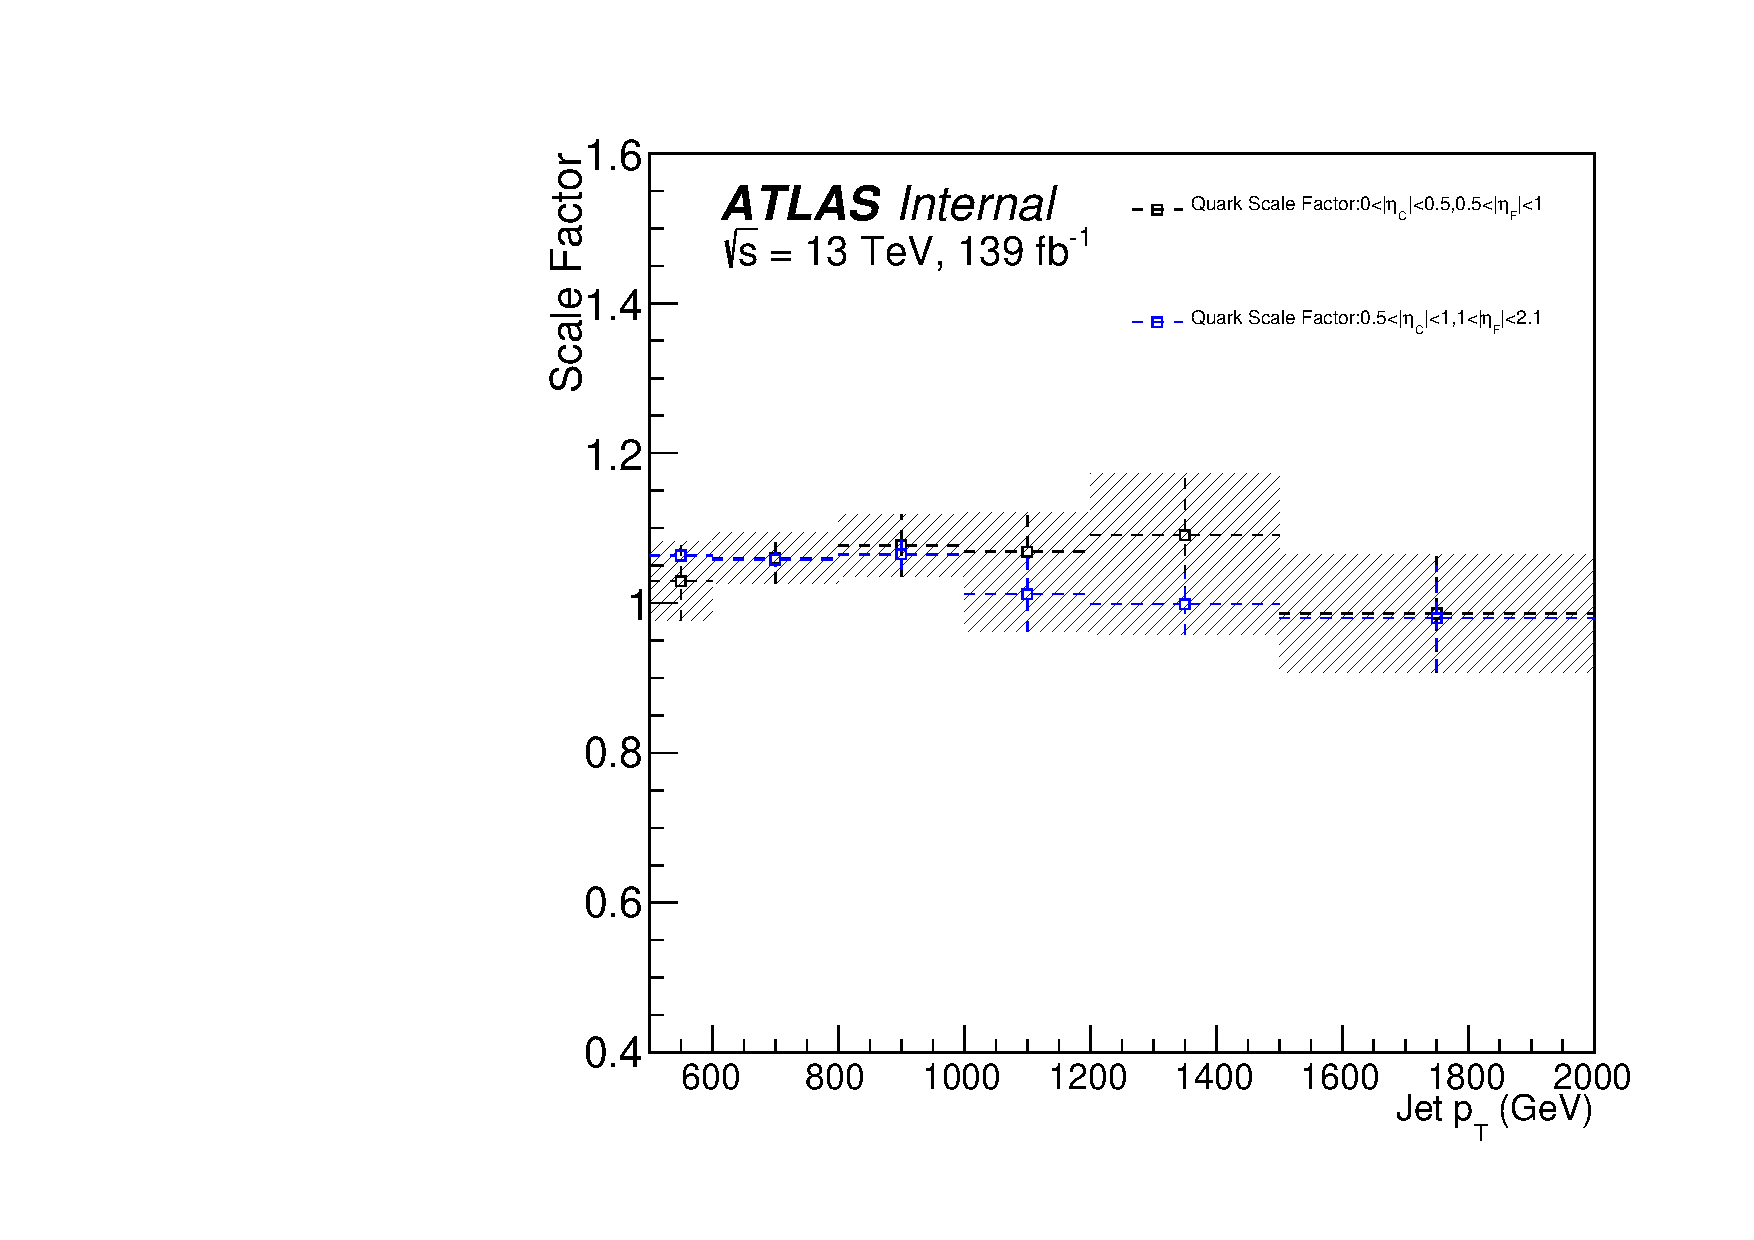
\includegraphics[width=0.45\textwidth]{fig/Method1/pythia/eta/working-point-SF-compare/0-0.5_0.5-1_0.5-1_1-2.1-Quark-SF-0.6-bdt.pdf}}\\
%	\subfloat[Gluon,Working Point:60\%~(\pythia8)]{\label{fig:QG-pythia-BDTDataGWP}\includegraphics[width=0.45\textwidth]{fig/Method1/pythia/eta/working-point-SF-compare/0-0.5_0.5-1_0.5-1_1-2.1-Gluon-WP-0.6-bdt.pdf}} \quad
%	\subfloat[Gluon,Working Point:60\%~(\pythia8)]{\label{fig:QG-pythia-BDTDataGSF}\includegraphics[width=0.45\textwidth]{fig/Method1/pythia/eta/working-point-SF-compare/0-0.5_0.5-1_0.5-1_1-2.1-Gluon-SF-0.6-bdt.pdf}}\\
%	\caption[]{
%	For 60$\%$ working point of BDT ,compare quark efficiency,gluon rejection and scale factors in 0<$\mid\eta_{C}\mid$<0.5,0.5<$\mid\eta_{F}\mid$<1 and in 0.5<$\mid\eta_{C}\mid$<1,1<$\mid\eta_{F}\mid$<2.1.%
%	The left plots are for quark efficiency and quark scale factors.The right plots are for gluon rejection and gluon scale factors. %
%	\subref{fig:QG-pythia-BDTDataQWP}  \subref{fig:QG-pythia-BDTDataQSF} are for quark distribution and \subref{fig:QG-pythia-BDTDataGWP}  \subref{fig:QG-pythia-BDTDataGSF} are for gluon distribution. %
% 	The error bars include the statistical uncertainty for quark efficiency and gluon factor and include statistical and parton shower modeling uncertainty for scale factors. %
%		\label{fig:QG-pythia-eta-BDT-6}
%	}
%\end{figure}
%
%\begin{figure}[htb]
%	\centering
%	\subfloat[Quark,Working Point:70\%~(\pythia8)]{\label{fig:QG-pythia-BDTDataQWP}\includegraphics[width=0.45\textwidth]{fig/Method1/pythia/eta/working-point-SF-compare/0-0.5_0.5-1_0.5-1_1-2.1-Quark-WP-0.7-bdt.pdf}} \quad
%	\subfloat[Quark,Working Point:70\%~(\pythia8)]{\label{fig:QG-pythia-BDTDataQSF}\includegraphics[width=0.45\textwidth]{fig/Method1/pythia/eta/working-point-SF-compare/0-0.5_0.5-1_0.5-1_1-2.1-Quark-SF-0.7-bdt.pdf}}\\
%	\subfloat[Gluon,Working Point:70\%~(\pythia8)]{\label{fig:QG-pythia-BDTDataGWP}\includegraphics[width=0.45\textwidth]{fig/Method1/pythia/eta/working-point-SF-compare/0-0.5_0.5-1_0.5-1_1-2.1-Gluon-WP-0.7-bdt.pdf}} \quad
%	\subfloat[Gluon,Working Point:70\%~(\pythia8)]{\label{fig:QG-pythia-BDTDataGSF}\includegraphics[width=0.45\textwidth]{fig/Method1/pythia/eta/working-point-SF-compare/0-0.5_0.5-1_0.5-1_1-2.1-Gluon-SF-0.7-bdt.pdf}}\\
%	\caption[]{
%	For 70$\%$ working point of BDT,compare quark efficiency,gluon rejection and scale factors in 0<$\mid\eta_{C}\mid$<0.5,0.5<$\mid\eta_{F}\mid$<1 and in 0.5<$\mid\eta_{C}\mid$<1,1<$\mid\eta_{F}\mid$<2.1.%
%	The left plots are for quark efficiency and quark scale factors.The right plots are for gluon rejection and gluon scale factors. %
%	\subref{fig:QG-pythia-BDTDataQWP}  \subref{fig:QG-pythia-BDTDataQSF} are for quark distribution and \subref{fig:QG-pythia-BDTDataGWP}  \subref{fig:QG-pythia-BDTDataGSF} are for gluon distribution. %
% 	The error bars include the statistical uncertainty for quark efficiency and gluon factor and include statistical and parton shower modeling uncertainty for scale factors. %
%		\label{fig:QG-pythia-eta-BDT-7}
%	}
%\end{figure}
%
%\begin{figure}[htb]
%	\centering
%	\subfloat[Quark,Working Point:80\%~(\pythia8)]{\label{fig:QG-pythia-BDTDataQWP}\includegraphics[width=0.45\textwidth]{fig/Method1/pythia/eta/working-point-SF-compare/0-0.5_0.5-1_0.5-1_1-2.1-Quark-WP-0.8-bdt.pdf}} \quad
%	\subfloat[Quark,Working Point:80\%~(\pythia8)]{\label{fig:QG-pythia-BDTDataQSF}\includegraphics[width=0.45\textwidth]{fig/Method1/pythia/eta/working-point-SF-compare/0-0.5_0.5-1_0.5-1_1-2.1-Quark-SF-0.8-bdt.pdf}}\\
%	\subfloat[Gluon,Working Point:80\%~(\pythia8)]{\label{fig:QG-pythia-BDTDataGWP}\includegraphics[width=0.45\textwidth]{fig/Method1/pythia/eta/working-point-SF-compare/0-0.5_0.5-1_0.5-1_1-2.1-Gluon-WP-0.8-bdt.pdf}} \quad
%	\subfloat[Gluon,Working Point:80\%~(\pythia8)]{\label{fig:QG-pythia-BDTDataGSF}\includegraphics[width=0.45\textwidth]{fig/Method1/pythia/eta/working-point-SF-compare/0-0.5_0.5-1_0.5-1_1-2.1-Gluon-SF-0.8-bdt.pdf}}\\
%	\caption[]{
%	For 80$\%$ working point of BDT ,compare quark efficiency,gluon rejection and scale factors in 0<$\mid\eta_{C}\mid$<0.5,0.5<$\mid\eta_{F}\mid$<1 and in 0.5<$\mid\eta_{C}\mid$<1,1<$\mid\eta_{F}\mid$<2.1.%
%	The left plots are for quark efficiency and quark scale factors.The right plots are for gluon rejection and gluon scale factors. %
%	\subref{fig:QG-pythia-BDTDataQWP}  \subref{fig:QG-pythia-BDTDataQSF} are for quark distribution and \subref{fig:QG-pythia-BDTDataGWP}  \subref{fig:QG-pythia-BDTDataGSF} are for gluon distribution. %
% 	The error bars include the statistical uncertainty for quark efficiency and gluon factor and include statistical and parton shower modeling uncertainty for scale factors. %
%		\label{fig:QG-pythia-eta-BDT-8}
%	}
%\end{figure}
%The quark efficiency , gluon rejection and scale factors for different eta range are shown from Fig.~\ref{fig:QG-pythia-etas-NtrkWPeta500-compare1} to Fig.~\ref{fig:QG-pythia-etas-BDTWPeta800-compare2} for \ntrk and BDT . The eta range is divided into 6 regions:
%(1) $0 < \mid\eta_{C}\mid < 0.5,0.5 < \mid\eta_{F}\mid < 1$ (2) 0 < $\mid\eta_{C}\mid$ < 0.5,1 < $\mid\eta_{F}\mid$ < 1.5 (3) 0 < $\mid\eta_{C}\mid$ < 0.5,1.5 < $\mid\eta_{F}\mid$ < 2.1 (4) 0.5 < $\mid\eta_{C}\mid$ < 1,1 < $\mid\eta_{F}\mid$ < 1.5  (5) 0.5 < $\mid\eta_{C}\mid$ < 1 , 1.5 < $\mid\eta_{F}\mid$ < 2.1 (6)  1 < $\mid\eta_{C}\mid$ < 1.5 , 1.5 < $\mid\eta_{F}\mid$ < 2.1.
%
%\begin{figure}[htb]
%	\centering
%	\subfloat[Working Point:50\%~(\pythia8)]{\label{fig:QG-pythia-NtrkDataQa}\includegraphics[width=0.45\textwidth]{fig/Method1/pythia/eta/WP-SF-sho/500-quark-0.5-ntrk-rej-show.pdf}} \quad
%	\subfloat[Working Point:50\%~(\pythia8)]{\label{fig:QG-pythia-NtrkDataGa}\includegraphics[width=0.45\textwidth]{fig/Method1/pythia/eta/WP-SF-sho/500-gluon-0.5-ntrk-rej-show.pdf}}\\
%	\subfloat[Working Point:60\%~(\pythia8)]{\label{fig:QG-pythia-NtrkDataQb}\includegraphics[width=0.45\textwidth]{fig/Method1/pythia/eta/WP-SF-sho/500-quark-0.6-ntrk-rej-show.pdf}} \quad
%	\subfloat[Working Point:60\%~(\pythia8)]{\label{fig:QG-pythia-NtrkDataGb}\includegraphics[width=0.45\textwidth]{fig/Method1/pythia/eta/WP-SF-sho/500-gluon-0.6-ntrk-rej-show.pdf}}\\
%	\caption[]{
%	Compare the quark efficiency , gluon rejection and scale factors in 500-600GeV in different $\eta$ range by working point of 50\%  $\ntrk$  quark jets efficiency \subref{fig:QG-pythia-NtrkDataQa} \subref{fig:QG-pythia-NtrkDataGa}  and by working point of 60\%  $\ntrk$  quark jets efficiency \subref{fig:QG-pythia-NtrkDataQb} \subref{fig:QG-pythia-NtrkDataGb}.
%	The error bars include the statistical uncertainty for quark efficiency and gluon rejection and include statistical and parton shower modeling uncertainty for scale factors. %
%	\label{fig:QG-pythia-etas-NtrkWPeta500-compare1}
%	}
%\end{figure}
%
%\begin{figure}[htb]
%	\centering
%	\subfloat[Working Point:70\%~(\pythia8)]{\label{fig:QG-pythia-NtrkDataQa}\includegraphics[width=0.45\textwidth]{fig/Method1/pythia/eta/WP-SF-sho/500-quark-0.7-ntrk-rej-show.pdf}} \quad
%	\subfloat[Working Point:70\%~(\pythia8)]{\label{fig:QG-pythia-NtrkDataGa}\includegraphics[width=0.45\textwidth]{fig/Method1/pythia/eta/WP-SF-sho/500-gluon-0.7-ntrk-rej-show.pdf}}\\
%	\subfloat[Working Point:80\%~(\pythia8)]{\label{fig:QG-pythia-NtrkDataQb}\includegraphics[width=0.45\textwidth]{fig/Method1/pythia/eta/WP-SF-sho/500-quark-0.8-ntrk-rej-show.pdf}} \quad
%	\subfloat[Working Point:80\%~(\pythia8)]{\label{fig:QG-pythia-NtrkDataGb}\includegraphics[width=0.45\textwidth]{fig/Method1/pythia/eta/WP-SF-sho/500-gluon-0.8-ntrk-rej-show.pdf}}\\
%	\caption[]{
%	Compare the quark efficiency , gluon rejection and scale factors in 500-600GeV in different $\eta$ range by working point of 70\%  $\ntrk$  quark jets efficiency \subref{fig:QG-pythia-NtrkDataQa} \subref{fig:QG-pythia-NtrkDataGa}  and by working point of 80\%  $\ntrk$  quark jets efficiency \subref{fig:QG-pythia-NtrkDataQb} \subref{fig:QG-pythia-NtrkDataGb}.
%	The error bars include the statistical uncertainty for quark efficiency and gluon rejection and include statistical and parton shower modeling uncertainty for scale factors. %
%	\label{fig:QG-pythia-etas-NtrkWPeta500-compare2}
%	}
%\end{figure}
%
%\begin{figure}[htb]
%	\centering
%	\subfloat[Working Point:50\%~(\pythia8)]{\label{fig:QG-pythia-BDTDataQa}\includegraphics[width=0.45\textwidth]{fig/Method1/pythia/eta/WP-SF-sho/500-quark-0.5-bdt-rej-show.pdf}} \quad
%	\subfloat[Working Point:50\%~(\pythia8)]{\label{fig:QG-pythia-BDTDataGa}\includegraphics[width=0.45\textwidth]{fig/Method1/pythia/eta/WP-SF-sho/500-gluon-0.5-bdt-rej-show.pdf}}\\
%	\subfloat[Working Point:60\%~(\pythia8)]{\label{fig:QG-pythia-BDTDataQb}\includegraphics[width=0.45\textwidth]{fig/Method1/pythia/eta/WP-SF-sho/500-quark-0.6-bdt-rej-show.pdf}} \quad
%	\subfloat[Working Point:60\%~(\pythia8)]{\label{fig:QG-pythia-BDTDataGb}\includegraphics[width=0.45\textwidth]{fig/Method1/pythia/eta/WP-SF-sho/500-gluon-0.6-bdt-rej-show.pdf}}\\
%	\caption[]{
%	Compare the quark efficiency , gluon rejection and scale factors in 500-600GeV in different $\eta$ range by working point of 50\%  BDT  quark jets efficiency \subref{fig:QG-pythia-BDTDataQa} \subref{fig:QG-pythia-BDTDataGa}  and by working point of 60\%  BDT  quark jets efficiency \subref{fig:QG-pythia-BDTDataQb} \subref{fig:QG-pythia-BDTDataGb}.
%	The error bars include the statistical uncertainty for quark efficiency and gluon rejection and include statistical and parton shower modeling uncertainty for scale factors. %
%	\label{fig:QG-pythia-etas-BDTWPeta500-compare1}
%	}
%\end{figure}
%
%\begin{figure}[htb]
%	\centering
%	\subfloat[Working Point:70\%~(\pythia8)]{\label{fig:QG-pythia-BDTDataQa}\includegraphics[width=0.45\textwidth]{fig/Method1/pythia/eta/WP-SF-sho/500-quark-0.7-bdt-rej-show.pdf}} \quad
%	\subfloat[Working Point:70\%~(\pythia8)]{\label{fig:QG-pythia-BDTDataGa}\includegraphics[width=0.45\textwidth]{fig/Method1/pythia/eta/WP-SF-sho/500-gluon-0.7-bdt-rej-show.pdf}}\\
%	\subfloat[Working Point:80\%~(\pythia8)]{\label{fig:QG-pythia-BDTDataQb}\includegraphics[width=0.45\textwidth]{fig/Method1/pythia/eta/WP-SF-sho/500-quark-0.8-bdt-rej-show.pdf}} \quad
%	\subfloat[Working Point:80\%~(\pythia8)]{\label{fig:QG-pythia-BDTDataGb}\includegraphics[width=0.45\textwidth]{fig/Method1/pythia/eta/WP-SF-sho/500-gluon-0.8-bdt-rej-show.pdf}}\\
%	\caption[]{
%	Compare the quark efficiency , gluon rejection and scale factors in 500-600GeV in different $\eta$ range by working point of 70\%  BDT  quark jets efficiency \subref{fig:QG-pythia-BDTDataQa} \subref{fig:QG-pythia-BDTDataGa}  and by working point of 80\%  BDT  quark jets efficiency \subref{fig:QG-pythia-BDTDataQb} \subref{fig:QG-pythia-BDTDataGb}.
%	The error bars include the statistical uncertainty for quark efficiency and gluon rejection and include statistical and parton shower modeling uncertainty for scale factors. %
%	\label{fig:QG-pythia-etas-BDTWPeta500-compare2}
%	}
%\end{figure}
%
%\begin{figure}[htb]
%	\centering
%	\subfloat[Working Point:50\%~(\pythia8)]{\label{fig:QG-pythia-NtrkDataQa}\includegraphics[width=0.45\textwidth]{fig/Method1/pythia/eta/WP-SF-sho/800-quark-0.5-ntrk-rej-show.pdf}} \quad
%	\subfloat[Working Point:50\%~(\pythia8)]{\label{fig:QG-pythia-NtrkDataGa}\includegraphics[width=0.45\textwidth]{fig/Method1/pythia/eta/WP-SF-sho/800-gluon-0.5-ntrk-rej-show.pdf}}\\
%	\subfloat[Working Point:60\%~(\pythia8)]{\label{fig:QG-pythia-NtrkDataQb}\includegraphics[width=0.45\textwidth]{fig/Method1/pythia/eta/WP-SF-sho/800-quark-0.6-ntrk-rej-show.pdf}} \quad
%	\subfloat[Working Point:60\%~(\pythia8)]{\label{fig:QG-pythia-NtrkDataGb}\includegraphics[width=0.45\textwidth]{fig/Method1/pythia/eta/WP-SF-sho/800-gluon-0.6-ntrk-rej-show.pdf}}\\
%	\caption[]{
%	Compare the quark efficiency , gluon rejection and scale factors in 800-1000GeV in different $\eta$ range by working point of 50\%  $\ntrk$  quark jets efficiency \subref{fig:QG-pythia-NtrkDataQa} \subref{fig:QG-pythia-NtrkDataGa}  and by working point of 60\%  $\ntrk$  quark jets efficiency \subref{fig:QG-pythia-NtrkDataQb} \subref{fig:QG-pythia-NtrkDataGb}.
%	The error bars include the statistical uncertainty for quark efficiency and gluon rejection and include statistical and parton shower modeling uncertainty for scale factors. %
%	\label{fig:QG-pythia-etas-NtrkWPeta800-compare1}
%	}
%\end{figure}
%
%\begin{figure}[htb]
%	\centering
%	\subfloat[Working Point:70\%~(\pythia8)]{\label{fig:QG-pythia-NtrkDataQa}\includegraphics[width=0.45\textwidth]{fig/Method1/pythia/eta/WP-SF-sho/800-quark-0.7-ntrk-rej-show.pdf}} \quad
%	\subfloat[Working Point:70\%~(\pythia8)]{\label{fig:QG-pythia-NtrkDataGa}\includegraphics[width=0.45\textwidth]{fig/Method1/pythia/eta/WP-SF-sho/800-gluon-0.7-ntrk-rej-show.pdf}}\\
%	\subfloat[Working Point:80\%~(\pythia8)]{\label{fig:QG-pythia-NtrkDataQb}\includegraphics[width=0.45\textwidth]{fig/Method1/pythia/eta/WP-SF-sho/800-quark-0.8-ntrk-rej-show.pdf}} \quad
%	\subfloat[Working Point:80\%~(\pythia8)]{\label{fig:QG-pythia-NtrkDataGb}\includegraphics[width=0.45\textwidth]{fig/Method1/pythia/eta/WP-SF-sho/800-gluon-0.8-ntrk-rej-show.pdf}}\\
%	\caption[]{
%	Compare the quark efficiency , gluon rejection and scale factors in 800-1000GeV in different $\eta$ range by working point of 70\%  $\ntrk$  quark jets efficiency \subref{fig:QG-pythia-NtrkDataQa} \subref{fig:QG-pythia-NtrkDataGa}  and by working point of 80\%  $\ntrk$  quark jets efficiency \subref{fig:QG-pythia-NtrkDataQb} \subref{fig:QG-pythia-NtrkDataGb}.
%	The error bars include the statistical uncertainty for quark efficiency and gluon rejection and include statistical and parton shower modeling uncertainty for scale factors. %
%	\label{fig:QG-pythia-etas-NtrkWPeta800-compare2}
%	}
%\end{figure}
%
%\begin{figure}[htb]
%	\centering
%	\subfloat[Working Point:50\%~(\pythia8)]{\label{fig:QG-pythia-BDTDataQa}\includegraphics[width=0.45\textwidth]{fig/Method1/pythia/eta/WP-SF-sho/800-quark-0.5-bdt-rej-show.pdf}} \quad
%	\subfloat[Working Point:50\%~(\pythia8)]{\label{fig:QG-pythia-BDTDataGa}\includegraphics[width=0.45\textwidth]{fig/Method1/pythia/eta/WP-SF-sho/800-gluon-0.5-bdt-rej-show.pdf}}\\
%	\subfloat[Working Point:60\%~(\pythia8)]{\label{fig:QG-pythia-BDTDataQb}\includegraphics[width=0.45\textwidth]{fig/Method1/pythia/eta/WP-SF-sho/800-quark-0.6-bdt-rej-show.pdf}} \quad
%	\subfloat[Working Point:60\%~(\pythia8)]{\label{fig:QG-pythia-BDTDataGb}\includegraphics[width=0.45\textwidth]{fig/Method1/pythia/eta/WP-SF-sho/800-gluon-0.6-bdt-rej-show.pdf}}\\
%	\caption[]{
%	Compare the quark efficiency , gluon rejection and scale factors in 800-1000GeV in different $\eta$ range by working point of 50\%  BDT  quark jets efficiency \subref{fig:QG-pythia-BDTDataQa} \subref{fig:QG-pythia-BDTDataGa}  and by working point of 60\%  BDT  quark jets efficiency \subref{fig:QG-pythia-BDTDataQb} \subref{fig:QG-pythia-BDTDataGb}.
%	The error bars include the statistical uncertainty for quark efficiency and gluon rejection and include statistical and parton shower modeling uncertainty for scale factors. %
%	\label{fig:QG-pythia-etas-BDTWPeta800-compare1}
%	}
%\end{figure}
%
%\begin{figure}[htb]
%	\centering
%	\subfloat[Working Point:70\%~(\pythia8)]{\label{fig:QG-pythia-BDTDataQa}\includegraphics[width=0.45\textwidth]{fig/Method1/pythia/eta/WP-SF-sho/800-quark-0.7-bdt-rej-show.pdf}} \quad
%	\subfloat[Working Point:70\%~(\pythia8)]{\label{fig:QG-pythia-BDTDataGa}\includegraphics[width=0.45\textwidth]{fig/Method1/pythia/eta/WP-SF-sho/800-gluon-0.7-bdt-rej-show.pdf}}\\
%	\subfloat[Working Point:80\%~(\pythia8)]{\label{fig:QG-pythia-BDTDataQb}\includegraphics[width=0.45\textwidth]{fig/Method1/pythia/eta/WP-SF-sho/800-quark-0.8-bdt-rej-show.pdf}} \quad
%	\subfloat[Working Point:80\%~(\pythia8)]{\label{fig:QG-pythia-BDTDataGb}\includegraphics[width=0.45\textwidth]{fig/Method1/pythia/eta/WP-SF-sho/800-gluon-0.8-bdt-rej-show.pdf}}\\
%	\caption[]{
%	Compare the quark efficiency , gluon rejection and scale factors in 800-1000GeV in different $\eta$ range by working point of 70\%  BDT  quark jets efficiency \subref{fig:QG-pythia-BDTDataQa} \subref{fig:QG-pythia-BDTDataGa}  and by working point of 80\%  BDT  quark jets efficiency \subref{fig:QG-pythia-BDTDataQb} \subref{fig:QG-pythia-BDTDataGb}.
%	The error bars include the statistical uncertainty for quark efficiency and gluon rejection and include statistical and parton shower modeling uncertainty for scale factors. %
%	\label{fig:QG-pythia-etas-BDTWPeta800-compare2}
%	}
%\end{figure}

